\documentclass[12pt,a4paper]{report}

% ── Encodage & langue ────────────────────────────────────────────────────────
\usepackage[utf8]{inputenc}
\usepackage[T1]{fontenc}
\usepackage[french]{babel}
\usepackage{mathptmx}          % Times New Roman (charte §3.2)

% ── Mise en page ─────────────────────────────────────────────────────────────
\usepackage[
a4paper,
top=2.5cm,
bottom=2.5cm,
left=3cm,
right=2cm,
headheight=15pt,
includeheadfoot
]{geometry}

\usepackage{setspace}
\onehalfspacing                    % Interligne 1.5

\setlength{\parindent}{0.5cm}      % Indentation paragraphe (charte §3.3)
\setlength{\parskip}{0.5em}        % Espace entre paragraphes

% ── Graphiques & couleurs ────────────────────────────────────────────────────
\usepackage{graphicx}
\usepackage{xcolor}
\usepackage{tikz}
\usetikzlibrary{shapes,arrows,positioning,fit,backgrounds,decorations.pathreplacing}
\graphicspath{{emage/}}

% ── Tableaux ─────────────────────────────────────────────────────────────────
\usepackage{booktabs}
\usepackage{tabularx}
\usepackage{longtable}
\usepackage{multirow}
\usepackage{array}
\usepackage{colortbl}
\usepackage{makecell}

% ── Code source ──────────────────────────────────────────────────────────────
\usepackage{listings}
\lstset{
	basicstyle=\small\ttfamily,
	backgroundcolor=\color{gray!8},
	frame=single,
	rulecolor=\color{gray!40},
	breaklines=true,
	breakatwhitespace=true,
	numbers=left,
	numberstyle=\tiny\color{gray},
	numbersep=6pt,
	keywordstyle=\color{blue!70}\bfseries,
	commentstyle=\color{green!50!black}\itshape,
	stringstyle=\color{orange!80!black},
	showstringspaces=false,
	tabsize=2,
	extendedchars=true,
	inputencoding=utf8,
	literate=
	{é}{{\'{e}}}1 {è}{{\`{e}}}1 {ê}{{\^{e}}}1 {ë}{{\"e}}1
	{à}{{\`{a}}}1 {â}{{\^{a}}}1 {ä}{{\"a}}1
	{î}{{\^{i}}}1 {ï}{{\"i}}1
	{ô}{{\^{o}}}1 {ö}{{\"o}}1
	{ù}{{\`{u}}}1 {û}{{\^{u}}}1 {ü}{{\"u}}1
	{ç}{{\c{c}}}1
	{É}{{\'{E}}}1 {È}{{\`{E}}}1 {Ê}{{\^{E}}}1
	{À}{{\`{A}}}1 {Â}{{\^{A}}}1
	{Î}{{\^{I}}}1 {Ô}{{\^{O}}}1
	{Ù}{{\`{U}}}1 {Û}{{\^{U}}}1
	{Ç}{{\c{C}}}1,
}

% ── Liens & PDF ──────────────────────────────────────────────────────────────
\usepackage{hyperref}
\hypersetup{
	colorlinks=true,
	linkcolor=bleuMain,
	citecolor=bleuMain,
	urlcolor=bleuLight,
	pdftitle={Rapport PFE -- Tableau de bord décisionnel CHU Ibn Sina},
	pdfauthor={Azddine},
}

% ── En-têtes & pieds de page ─────────────────────────────────────────────────
\usepackage{fancyhdr}
\usepackage{truncate}
\pagestyle{fancy}
\fancyhf{}
\fancyhead[L]{\fontsize{9}{11}\selectfont\itshape\truncate{0.55\textwidth}{\leftmark}}
\fancyhead[R]{\fontsize{9}{11}\selectfont\itshape CHU Ibn Sina}
\fancyfoot[L]{\fontsize{9}{11}\selectfont\itshape PFE 2025/2026}
\fancyfoot[C]{\fontsize{9}{11}\selectfont\thepage}
\renewcommand{\headrulewidth}{0.4pt}
\renewcommand{\footrulewidth}{0.2pt}

% ── Listes & énumérations ────────────────────────────────────────────────────
\usepackage{enumitem}
\usepackage{amssymb}
\usepackage{amsmath}

% ── Divers ───────────────────────────────────────────────────────────────────
\usepackage{float}
\usepackage{caption}
\usepackage{subcaption}
% Légendes : 10pt italique, séparateur " : " style français (charte §3.2 + §7.1)
\DeclareCaptionLabelSeparator{francais}{ : }
\captionsetup{font={footnotesize,it}, labelfont=bf, labelsep=francais}
\captionsetup[table]{position=above}
\captionsetup[figure]{position=below}
\usepackage{tocloft}
\usepackage{etoc}
\usepackage{pdfpages}
\usepackage{needspace}
\usepackage{etoolbox}
\usepackage{eso-pic}

% ── Empêcher les titres seuls en bas de page ─────────────────────────────────
\widowpenalty=10000
\clubpenalty=10000
\preto{\section}{\needspace{6\baselineskip}}
\preto{\subsection}{\needspace{5\baselineskip}}
\preto{\subsubsection}{\needspace{4\baselineskip}}
\usepackage{mdframed}
\usepackage{pgfplots}
\pgfplotsset{compat=1.18}

% ── Couleurs personnalisées ──────────────────────────────────────────────────
\definecolor{bleuCHU}{RGB}{15,23,41}
\definecolor{bleuMain}{RGB}{26,49,112}
\definecolor{bleuLight}{RGB}{59,130,246}
\definecolor{grisLight}{RGB}{243,244,246}
\definecolor{vertOK}{RGB}{22,163,74}
\definecolor{orange}{RGB}{234,88,12}
\definecolor{rouge}{RGB}{220,38,38}
\definecolor{violet}{RGB}{124,58,237}
\definecolor{jaune}{RGB}{234,179,8}

% ── Style des chapitres (charte §3.2 : Titre chapitre=14pt gras, section=12pt gras) ──
\usepackage{titlesec}
\titleformat{\chapter}[display]
{\normalfont\fontsize{14}{16}\selectfont\bfseries\color{bleuMain}}
{\chaptertitlename\ \thechapter}{12pt}{\fontsize{14}{16}\selectfont}
\titlespacing*{\chapter}{0pt}{30pt}{12pt}
\titleformat{\section}{\normalfont\fontsize{12}{14}\selectfont\bfseries\color{bleuMain}}{\thesection}{1em}{}
\titlespacing*{\section}{0pt}{*2}{12pt}
\titleformat{\subsection}{\normalfont\fontsize{12}{14}\selectfont\bfseries\color{bleuLight}}{\thesubsection}{1em}{}
\titlespacing*{\subsection}{0pt}{*1.5}{12pt}
\titleformat{\subsubsection}{\normalfont\fontsize{12}{14}\selectfont\bfseries\color{bleuCHU}}{\thesubsubsection}{1em}{}
\titlespacing*{\subsubsection}{0pt}{*1}{12pt}

% ── Boîtes info / alerte ─────────────────────────────────────────────────────
\newmdenv[backgroundcolor=bleuLight!8,linecolor=bleuLight,linewidth=2pt,
leftline=true,rightline=false,topline=false,bottomline=false,
innerleftmargin=12pt,innertopmargin=8pt,innerbottommargin=8pt]{infobox}

\newmdenv[backgroundcolor=orange!8,linecolor=orange,linewidth=2pt,
leftline=true,rightline=false,topline=false,bottomline=false,
innerleftmargin=12pt,innertopmargin=8pt,innerbottommargin=8pt]{warnbox}

\newmdenv[backgroundcolor=vertOK!8,linecolor=vertOK,linewidth=2pt,
leftline=true,rightline=false,topline=false,bottomline=false,
innerleftmargin=12pt,innertopmargin=8pt,innerbottommargin=8pt]{successbox}

% ════════════════════════════════════════════════════════════════════════════
\begin{document}
	
	% ── Page de garde ────────────────────────────────────────────────────────────
	\begin{titlepage}
		\thispagestyle{empty}
		\newgeometry{top=0cm,bottom=0cm,left=0cm,right=0cm}
		
		% ── Fond (bg-img.jpg) ─────────────────────────────────────────────────────
		\AddToShipoutPictureBG*{%
			
\includegraphics[width=\paperwidth,height=\paperheight]{bg-img.jpg}%
		}
		
		% ── Bandeau logos : ISMAGI (bg) + CHU (overlay) ───────────────────────────
		% La zone logo du bg mesure ~3.5cm de hauteur
		\noindent
		\begin{minipage}[t][\paperwidth][t]{\paperwidth}
			
			% Ligne logos : espace à gauche (ISMAGI déjà dans le bg) + CHU à droite
			\hspace*{0.5cm}%
			\begin{minipage}[t]{0.55\textwidth}
				\vspace{0.6cm}  % aligner verticalement avec le bg
			\end{minipage}%
			\hfill
			\begin{minipage}[t]{0.35\textwidth}
				\vspace{0.4cm}
				\raggedleft
				\fboxsep=4pt\fboxrule=0.4pt
				\fbox{
\includegraphics[height=2.2cm]{CHU LOGO.PNG}}
				\hspace*{0.4cm}
			\end{minipage}
			
			% Espace pour la bande verte du bg (environ 3cm supplémentaires)
			\vspace{3.2cm}
			
			% ── Corps central ────────────────────────────────────────────────────────
			\begin{center}
				
				{\fontsize{26}{30}\selectfont \textbf{MÉMOIRE DE FIN D'ÉTUDE}}\\[0.5cm]
				
				{\normalsize En vue de l'obtention du diplôme de}\\[0.2cm]
				{\large \textbf{Ingénieur d'État en Génie Informatique}}\\[0.1cm]
				{\normalsize \textbf{Option : Business Intelligence \& Data Science}}\\[0.6cm]
				
				\noindent\rule{0.55\linewidth}{0.5pt}\\[0.4cm]
				
				{\normalsize \textbf{Sujet :}}\\[0.2cm]
				{\Large \bfseries \color{bleuMain}
					Tableau de Bord Décisionnel\\[0.15cm]
					pour la Gestion des Urgences Hospitalières\\[0.15cm]
					du CHU Ibn Sina de Rabat
				}\\[0.2cm]
				{\small \textit{Application Full-Stack · Pipeline ETL Medallion · Machine Learning}}
				
				\noindent\rule{0.55\linewidth}{0.5pt}\\[0.5cm]
				
				{\normalsize \textbf{Réalisé par :} \quad \large \textbf{Azddine Salim}}\\[0.25cm]
				{\small \textbf{Organisme d'accueil :} \quad CHU Ibn Sina -- Rabat}\\[0.6cm]
				
				{\normalsize \textit{Soutenu devant le jury composé de :}}\\[0.5cm]
				\renewcommand{\arraystretch}{1.6}
				\begin{tabular}{|>{\bfseries\color{bleuMain}}p{4cm}|p{6.5cm}|}
					\hline
					\rowcolor{bleuMain!10}
					Président(e)      & MINAOUI Khalid      \\
					\hline
					Encadrant(e)      & LAZAAR Mohammed     \\
					\hline
					Examinateur(trice)& ZIDANE Issam Eddine \\
					\hline
				\end{tabular}\\[0.6cm]
				
				{\normalsize \textit{Année universitaire :} \quad \textbf{2025 -- 2026}}
				
			\end{center}
			
		\end{minipage}
		
	\end{titlepage}
	\restoregeometry
	\ClearShipoutPictureBG
	
	% Pages préliminaires : numérotation romaine (charte §3.4)
	\pagenumbering{roman}
	\pagestyle{fancy}
	
	% ── Remerciements ────────────────────────────────────────────────────────────
	\chapter*{Remerciements}
	\addcontentsline{toc}{chapter}{Remerciements}
	\markboth{Remerciements}{}
	
	Je tiens à exprimer ma profonde gratitude à l'ensemble des personnes qui ont contribué,
	de près ou de loin, à la réalisation de ce projet de fin d'études.
	
	Mes premiers remerciements vont à la direction du \textbf{CHU Ibn Sina de Rabat} pour
	m'avoir accordé cette opportunité de stage et pour avoir mis à disposition toutes les
	ressources nécessaires à la bonne conduite de ce projet.
	
	Je remercie tout particulièrement mon encadrant pour ses conseils avisés, sa disponibilité
	constante et son suivi rigoureux tout au long de ce travail. Ses orientations ont été
	déterminantes dans la réussite de ce projet.
	
	Mes remerciements s'adressent également à l'équipe médicale et administrative du CHU qui
	a répondu à mes questions avec patience et m'a aidé à mieux comprendre les besoins réels
	du terrain. Les échanges avec les médecins urgentistes ont été particulièrement enrichissants
	pour définir les indicateurs pertinents.
	
	Je remercie aussi l'équipe informatique du CHU pour son soutien technique lors de la
	configuration de l'environnement de développement et de l'accès aux données.
	
	Enfin, je tiens à remercier le corps enseignant de ma formation BI \& Data Science pour
	la qualité de l'enseignement dispensé, qui m'a fourni les outils conceptuels et techniques
	indispensables à la réalisation de ce projet ambitieux.
	
	% ── Dédicace ─────────────────────────────────────────────────────────────────
	\chapter*{Dédicace}
	\addcontentsline{toc}{chapter}{Dédicace}
	\markboth{Dédicace}{}
	
	\begin{center}
		\vspace*{1.5cm}
		\textit{\Large À mes chers parents,}\\[0.6cm]
		{\normalsize
			Pour tous leurs sacrifices consentis tout au long de ma vie,\\
			pour leur amour inconditionnel, leur soutien sans faille\\
			et leur confiance indéfectible en mes capacités.\\
			Chaque réussite de ma vie vous est dédiée.\\[1cm]
		}
		\textit{\Large À ma famille,}\\[0.6cm]
		{\normalsize
			Pour leurs encouragements constants, leur présence indéfectible\\
			et l'énergie positive qu'ils m'ont transmise dans les moments difficiles.\\[1cm]
		}
		\textit{\Large À mes ami(e)s fidèles,}\\[0.6cm]
		{\normalsize
			Pour les moments partagés, les conseils précieux et la motivation mutuelle\\
			tout au long de ce parcours académique et professionnel.\\[1cm]
		}
		\textit{\Large À tous ceux et celles qui ont cru en moi\\
			et m'ont encouragé à me dépasser.}
	\end{center}
	
	% ── Résumé ───────────────────────────────────────────────────────────────────
	\chapter*{Résumé}
	\addcontentsline{toc}{chapter}{Résumé}
	\markboth{Résumé}{}
	
	Ce projet de fin d'études s'inscrit dans le cadre d'un stage effectué au sein du
	\textbf{CHU Ibn Sina de Rabat}. Il porte sur la conception et le développement d'un
	\textbf{tableau de bord décisionnel interactif} destiné à optimiser la gestion des urgences
	hospitalières du plus grand réseau hospitalier universitaire du Maroc.
	
	Face à la croissance constante du volume de patients aux urgences et à la complexité
	grandissante de la gestion des ressources humaines et matérielles, un système d'aide à la
	décision basé sur les données s'avère indispensable. Ce projet propose une solution
	\textit{full-stack} innovante comprenant :
	
	\begin{itemize}[leftmargin=1.5cm]
		\item Un \textbf{pipeline ETL Medallion} structuré en trois couches (Bronze, Silver, Gold)
		permettant de nettoyer, valider et enrichir les données avant de les centraliser dans
		une base MySQL ;
		\item Un \textbf{backend FastAPI} (Python 3.11) exposant une API REST complète sécurisée
		par authentification JWT avec contrôle d'accès basé sur les rôles (RBAC) ;
		\item Un \textbf{frontend React} (TypeScript) offrant 15 pages de visualisation interactive
		avec actualisation automatique toutes les 30 secondes ;
		\item Des \textbf{modèles de Machine Learning} (XGBoost, Random Forest, Prophet) pour la
		prédiction des flux de patients et la planification des ressources ;
		\item Un \textbf{système de cache Parquet} réduisant le temps de démarrage de 30 secondes
		à moins d'une seconde ;
		\item Un \textbf{déploiement Docker Compose} garantissant la portabilité et la scalabilité.
	\end{itemize}
	
	L'application a été développée et validée sur un jeu de données réel de
	\textbf{530 914 passages aux urgences} sur la période 2019--2026, couvrant les 8 établissements
	du réseau CHU Ibn Sina. Le module de prédiction d'orientation, basé sur Random Forest,
	identifie l'issue probable du patient (Hospitalisation, Retour domicile, Fugue, Transfert)
	à partir des statistiques conditionnelles calculées sur l'historique réel.
	
	\textbf{Mots-clés :} Tableau de bord, Business Intelligence, ETL Medallion, Machine Learning,
	FastAPI, React TypeScript, Docker, Urgences hospitalières, CHU Ibn Sina, Prédiction.
	
	% ── Abstract (page séparée, charte §3.2 : titre chapitre 14pt gras) ──────────
	\chapter*{Abstract}
	\addcontentsline{toc}{chapter}{Abstract}
	\markboth{Abstract}{}
	
	This final year project, carried out at \textbf{CHU Ibn Sina} in Rabat, focuses on designing
	and developing an interactive decision-support dashboard to optimize emergency department
	management across Morocco's largest university hospital network.
	
	The solution integrates a \textbf{Medallion ETL pipeline} (Bronze / Silver / Gold), a
	JWT-secured \textbf{FastAPI REST backend} with role-based access control (RBAC), a
	\textbf{React TypeScript frontend} with 15 visualization pages, Machine Learning prediction
	models (\textbf{XGBoost} for hourly flux prediction, \textbf{Random Forest} for patient
	orientation, \textbf{Prophet} for 30-day time-series forecasting), a \textbf{Parquet cache}
	system reducing startup time from 30\,s to under 1\,s, and a full \textbf{Docker Compose}
	deployment.
	
	The system processes \textbf{530,914 real emergency visits} across 8 hospitals from 2019
	to 2026, achieving a best prediction score of R²\,=\,0.967 (XGBoost).
	
	\textbf{Keywords:} Dashboard, Business Intelligence, Medallion ETL, Machine Learning,
	FastAPI, React TypeScript, Docker, Hospital Emergency Management, CHU Ibn Sina, Prediction.
	\newpage
	% ── Sommaire (chapitres + sections, charte §2 position 3) ───────────────────
	% ── Table des matières complète (chapitres + sections + sous-sections) ───────
	\clearpage
	\etocsettocdepth{subsubsection}
	\renewcommand{\contentsname}{Table des matières}
	\etocsettocstyle{\chapter*{Table des matières}}{}
	\tableofcontents
	
	% ── Fin du document
	\newpage
	% ── Liste des figures & tableaux (charte §2 position 4) ─────────────────────
	\addcontentsline{toc}{chapter}{\listfigurename}
	\listoffigures
	\newpage
	\addcontentsline{toc}{chapter}{\listtablename}
	\listoftables
	
	% ── Liste des abréviations ───────────────────────────────────────────────────
	\chapter*{Liste des abréviations}
	\addcontentsline{toc}{chapter}{Liste des abréviations}
	\markboth{Liste des abréviations}{}
	
	\begin{longtable}{p{3.2cm} p{10.5cm}}
		\toprule
		\textbf{Abréviation} & \textbf{Signification} \\
		\midrule
		\endhead
		\midrule
		\multicolumn{2}{r}{\small\itshape Suite page suivante...}\\
		\endfoot
		\bottomrule
		\endlastfoot
		API     & Application Programming Interface \\
		BI      & Business Intelligence \\
		CHUIS   & Centre Hospitalier Universitaire Ibn Sina \\
		CHU     & Centre Hospitalier Universitaire \\
		CIN     & Carte d'Identité Nationale \\
		CORS    & Cross-Origin Resource Sharing \\
		CSV     & Comma-Separated Values \\
		DB      & Database (Base de données) \\
		Docker  & Plateforme de conteneurisation logicielle \\
		EDA     & Exploratory Data Analysis (Analyse Exploratoire des Données) \\
		ETL     & Extract, Transform, Load \\
		HIS     & Hôpital Ibn Sina \\
		HAY     & Hôpital Al Ayachi \\
		HAR     & Hôpital Ar-Razi \\
		HEN     & Hôpital des Enfants \\
		HSP     & Hôpital des Spécialités \\
		HMY     & Hôpital Moulay Youssef \\
		HMS     & Hôpital de Maternité Souissi \\
		HTTP    & HyperText Transfer Protocol \\
		IPP     & Identifiant Permanent du Patient \\
		JWT     & JSON Web Token \\
		KPI     & Key Performance Indicator \\
		ML      & Machine Learning (Apprentissage Automatique) \\
		MySQL   & Système de Gestion de Bases de Données Relationnelles \\
		ORM     & Object-Relational Mapping \\
		PFE     & Projet de Fin d'Études \\
		RBAC    & Role-Based Access Control \\
		REST    & Representational State Transfer \\
		RF      & Random Forest \\
		RMSE    & Root Mean Square Error \\
		MAE     & Mean Absolute Error \\
		SQL     & Structured Query Language \\
		SPA     & Single Page Application \\
		XGB     & XGBoost (eXtreme Gradient Boosting) \\
		XAMPP   & X Apache MySQL PHP Perl \\
	\end{longtable}
	
	% Numérotation arabe à partir de l'Introduction (charte §3.4)
	\cleardoublepage
	\pagenumbering{arabic}
	\setcounter{page}{1}
	
	% ════════════════════════════════════════════════════════════════════════════
	\chapter*{Introduction Générale}
	\addcontentsline{toc}{chapter}{Introduction Générale}
	\markboth{Introduction Générale}{}
	
	\section*{Contexte et motivation}
	
	Le secteur hospitalier marocain fait face à des défis croissants : augmentation de la demande
	de soins, contraintes budgétaires, gestion complexe des ressources humaines et matérielles.
	Les services des urgences, en tant que premier point de contact avec le système de santé,
	sont particulièrement concernés. Au Maroc, les urgences hospitalières enregistrent des millions
	de passages annuels, avec des variations importantes selon l'heure de la journée, le jour de
	la semaine et la saison.
	
	Dans ce contexte, le recours aux technologies de l'information et aux outils d'analyse de
	données est devenu un levier stratégique pour améliorer la performance hospitalière. La
	\textit{Business Intelligence} (BI) appliquée au domaine médical -- souvent appelée
	\textit{Health Intelligence} -- permet de transformer des volumes massifs de données cliniques
	et administratives en informations actionnables pour les décideurs.
	
	\section*{Problématique}
	
	Le CHU Ibn Sina de Rabat dispose de données riches sur ses activités d'urgences, mais ces
	données sont dispersées dans différents systèmes d'information hétérogènes. L'absence d'un
	outil de consolidation et de visualisation centralisé rend difficile :
	\begin{itemize}
		\item le suivi en temps réel de l'état des urgences ;
		\item l'anticipation des pics d'affluence ;
		\item l'optimisation de l'allocation des ressources (lits, personnel) ;
		\item la prise de décision rapide et informée par les responsables médicaux.
	\end{itemize}
	
	\section*{Objectifs du projet}
	
	Ce projet vise à concevoir et développer une solution complète répondant à ces besoins, en
	combinant les approches de la BI, du Data Engineering et du Machine Learning. L'application
	développée permet de centraliser, visualiser et analyser les données d'urgences, tout en
	offrant des capacités prédictives pour anticiper les flux.
	
	\section*{Organisation du rapport}
	
	Ce rapport est organisé en six chapitres :
	\begin{itemize}
		\item Le \textbf{Chapitre 1} présente le contexte général du stage, l'organisme d'accueil
		et la méthodologie adoptée ;
		\item Le \textbf{Chapitre 2} décrit le pipeline ETL Medallion mis en place ;
		\item Le \textbf{Chapitre 3} présente l'analyse exploratoire des données et les KPIs définis ;
		\item Le \textbf{Chapitre 4} détaille les modèles de Machine Learning développés ;
		\item Le \textbf{Chapitre 5} présente les visualisations et le tableau de bord ;
		\item Le \textbf{Chapitre 6} traite de la sécurité, des performances et du déploiement.
	\end{itemize}
	
	% ════════════════════════════════════════════════════════════════════════════
	\chapter{Contexte général du stage}
	
	\section{Introduction}
	Ce chapitre présente le cadre général dans lequel s'est déroulé notre stage de fin d'études.
	Nous commençons par la présentation détaillée du CHU Ibn Sina, puis nous exposons les
	objectifs et le cadrage du projet, avant de décrire les outils et la méthodologie adoptée.
	
	\section{Présentation de l'organisme d'accueil}
	
	\subsection{Présentation générale du CHU Ibn Sina}
	Le \textbf{Centre Hospitalier Universitaire Ibn Sina (CHUIS)} est le plus grand et le plus
	ancien établissement hospitalier universitaire du Maroc. Fondé en 1955, il est situé à Rabat,
	capitale du Royaume, et constitue un pôle de référence national pour les soins spécialisés,
	l'enseignement médical et la recherche scientifique.
	
	Le CHU Ibn Sina se distingue par plusieurs caractéristiques majeures :
	\begin{itemize}
		\item Plus de \textbf{2 500 lits d'hospitalisation} répartis sur 8 établissements ;
		\item Plus de \textbf{6 000 agents} dont environ 800 médecins spécialistes ;
		\item Une capacité d'accueil de plus de \textbf{800 000 consultations} par an ;
		\item Un réseau de \textbf{30 services médicaux et chirurgicaux} spécialisés.
	\end{itemize}
	
	\subsection{Les établissements du réseau}
	
	\begin{table}[H]
		\centering
		\caption{Établissements du réseau CHU Ibn Sina}
		\renewcommand{\arraystretch}{1.3}
		\begin{tabularx}{\textwidth}{lXc}
			\toprule
			\textbf{Établissement} & \textbf{Spécialités principales} & \textbf{Capacité (lits)} \\
			\midrule
			Hôpital Ibn Sina          & Médecine générale, Urgences, Chirurgie   & \textasciitilde 800 \\
			Hôpital des Enfants       & Pédiatrie, Chirurgie pédiatrique          & \textasciitilde 350 \\
			Hôpital Al Ayachi         & Chirurgie, Médecine interne, Traumatologie & \textasciitilde 400 \\
			Hôpital Ar-Razi           & Psychiatrie, Neurologie, Addiction        & \textasciitilde 300 \\
			Hôpital des Spécialités   & Oncologie, Cardiologie, Endocrinologie    & \textasciitilde 400 \\
			Hôpital Moulay Youssef    & Dermatologie, Ophtalmologie, ORL          & \textasciitilde 200 \\
			Maternité Souissi         & Obstétrique, Gynécologie, Maternité       & \textasciitilde 200 \\
			Maternité Les Orangers    & Planification familiale, Néonatologie     & \textasciitilde 150 \\
			\bottomrule
		\end{tabularx}
	\end{table}
	
	\subsection{Les missions du CHUIS}
	
	Le CHU Ibn Sina remplit trois missions fondamentales et complémentaires :
	
	\begin{enumerate}[leftmargin=1.5cm]
		\item \textbf{Mission de soins} : Offrir des soins de qualité à l'ensemble de la population,
		notamment des soins spécialisés et de haute technicité inaccessibles dans d'autres
		structures. Le CHUIS est la structure de référence nationale pour de nombreuses
		pathologies complexes ;
		\item \textbf{Mission d'enseignement} : Former les futurs professionnels de santé en
		étroite collaboration avec la Faculté de Médecine et de Pharmacie de Rabat. Des
		milliers d'étudiants en médecine, en pharmacie et en sciences infirmières y effectuent
		leurs stages pratiques chaque année ;
		\item \textbf{Mission de recherche} : Contribuer à l'avancement des connaissances médicales
		à travers des projets de recherche clinique et fondamentale, en partenariat avec des
		institutions nationales et internationales.
	\end{enumerate}
	
	\subsection{Contexte numérique et enjeux informatiques}
	
	Le CHUIS s'est engagé dans un processus de transformation numérique visant à améliorer
	l'efficacité de ses processus internes et la qualité des soins prodigués. Les principaux
	enjeux identifiés sont :
	
	\begin{itemize}
		\item L'intégration et la consolidation des données provenant de systèmes d'information
		hétérogènes (HIS, LIS, RIS) ;
		\item La mise en place d'outils de pilotage et d'aide à la décision pour les responsables ;
		\item La réduction des délais d'attente aux urgences par une meilleure gestion des flux ;
		\item L'optimisation de l'utilisation des ressources (lits, blocs opératoires, personnel).
	\end{itemize}
	
	\section{Analyse des besoins du projet}
	
	\subsection{Besoins fonctionnels}
	
	Les besoins fonctionnels ont été identifiés lors d'ateliers avec les équipes médicales
	et administratives du CHU :
	
	\begin{table}[H]
		\centering
		\caption{Besoins fonctionnels identifiés}
		\renewcommand{\arraystretch}{1.2}
		\begin{tabularx}{\textwidth}{clX}
			\toprule
			\textbf{Priorité} & \textbf{Besoin} & \textbf{Description} \\
			\midrule
			\cellcolor{rouge!20}Critique  & Suivi temps réel    & Visualiser l'état des urgences en direct \\
			\cellcolor{rouge!20}Critique  & KPIs globaux        & Calculer et afficher les indicateurs clés \\
			\cellcolor{orange!20}Haute    & Prédictions ML      & Anticiper les flux sur 30 jours \\
			\cellcolor{orange!20}Haute    & Gestion des lits    & Suivre et attribuer les lits disponibles \\
			\cellcolor{orange!20}Haute    & Alertes             & Notifier les dépassements de seuils \\
			\cellcolor{jaune!20}Moyenne   & Analyse temporelle  & Identifier les patterns d'affluence \\
			\cellcolor{jaune!20}Moyenne   & Export données      & Exporter en Excel/CSV pour rapports \\
			\cellcolor{vertOK!20}Basse    & Carte géographique  & Localiser les établissements \\
			\bottomrule
		\end{tabularx}
	\end{table}
	\newpage
	\subsection{Besoins non fonctionnels}
	
	\begin{itemize}
		\item \textbf{Performance} : Temps de réponse des API inférieur à 500\,ms ;
		\item \textbf{Disponibilité} : L'application doit être accessible 24\,h/24, 7\,j/7 ;
		\item \textbf{Sécurité} : Authentification obligatoire, données médicales protégées ;
		\item \textbf{Scalabilité} : Architecture capable de supporter la montée en charge ;
		\item \textbf{Maintenabilité} : Code modulaire, documenté et testable.
	\end{itemize}
	
	\section{Présentation du projet}
	
	\subsection{Objectifs}
	L'objectif principal est de développer une \textbf{application web décisionnelle complète}
	permettant d'optimiser la gestion des urgences au sein du CHU Ibn Sina. Les objectifs
	spécifiques sont :
	
	\begin{itemize}
		\item Centraliser 530~914 passages aux urgences (2019--2026) dans une base MySQL ;
		\item Fournir des tableaux de bord interactifs en temps réel mis à jour toutes les 30\,s ;
		\item Intégrer des modèles de prédiction pour anticiper les flux sur 30 jours ;
		\item Permettre le suivi individuel de chaque patient de l'admission à la sortie ;
		\item Recommander automatiquement les ressources (lits, médecins) selon la date cible.
	\end{itemize}
	
	\subsection{Livrables}
	\begin{enumerate}
		\item Pipeline ETL documenté (Bronze $\rightarrow$ Silver $\rightarrow$ Gold) ;
		\item Base de données MySQL peuplée (7 tables, \textasciitilde 1,27 million de lignes) ;
		\item Backend FastAPI avec 64 endpoints REST documentés (Swagger) ;
		\item Frontend React avec 15 pages de visualisation ;
		\item 3 modèles ML entraînés et sérialisés ;
		\item Application déployée via Docker Compose.
	\end{enumerate}
	
	\section{Outils et technologies utilisés}
	
	\begin{table}[H]
		\centering
		\caption{Stack technologique complète du projet}
		\renewcommand{\arraystretch}{1.2}
		\begin{tabularx}{\textwidth}{llX}
			\toprule
			\textbf{Catégorie} & \textbf{Technologie} & \textbf{Rôle et justification} \\
			\midrule
			\multirow{5}{*}{Backend}
			& Python 3.11       & Langage principal : écosystème ML riche \\
			& FastAPI           & API REST : performance, auto-documentation \\
			& SQLAlchemy        & ORM multi-DB : abstraction MySQL/SQLite \\
			& PyMySQL           & Driver MySQL natif pour Python \\
			& PyJWT             & Génération et validation des tokens JWT \\
			\midrule
			\multirow{4}{*}{Data \& ML}
			& pandas 3.0        & Manipulation et transformation des données \\
			& XGBoost           & Prédiction flux patients (gradient boosting) \\
			& scikit-learn      & Pipeline ML, métriques, Random Forest \\
			& Prophet (Meta)    & Prévision séries temporelles 30 jours \\
			\midrule
			\multirow{3}{*}{Frontend}
			& React 18 + TypeScript & SPA réactive avec typage statique \\
			& Recharts          & Graphiques natifs React \\
			& Axios             & Client HTTP pour les appels API \\
			\midrule
			\multirow{3}{*}{Infra}
			& Docker Compose    & Orchestration des conteneurs \\
			& MySQL (XAMPP)     & Base de données principale \\
			& Apache Parquet    & Cache binaire (démarrage $<$1\,s) \\
			\midrule
			\multirow{2}{*}{Sécurité}
			& JWT + RBAC        & Authentification et contrôle d'accès \\
			& SHA-256           & Hachage des mots de passe \\
			\bottomrule
		\end{tabularx}
	\end{table}
	\newpage
	\section{Méthodologie du projet}
	
	La méthodologie adoptée est de type \textbf{agile itérative}, organisée en 6 sprints
	de deux semaines chacun, pour une durée totale de 12 semaines.
	
	\subsection{Diagramme de Gantt}
	
	\begin{table}[H]
		\centering
		\caption{Planning du projet — Diagramme de Gantt avec dépendances (12 semaines)}
		\renewcommand{\arraystretch}{1.15}
		\small
		\begin{tabular}{l|c|cccccccccccc}
			\toprule
			\textbf{Tâche} & \textbf{Dépend de} & \multicolumn{12}{c}{\textbf{Semaines}} \\
			& & 1 & 2 & 3 & 4 & 5 & 6 & 7 & 8 & 9 & 10 & 11 & 12 \\
			\midrule
			1. Analyse des besoins   & —     & \cellcolor{bleuLight!60} & \cellcolor{bleuLight!60} & & & & & & & & & & \\
			2. Conception ETL        & (1)   & & \cellcolor{orange!50} & \cellcolor{orange!50} & & & & & & & & & \\
			3. Développement ETL     & (2)   & & & \cellcolor{orange!80} & \cellcolor{orange!80} & & & & & & & & \\
			4. Backend FastAPI       & (3)   & & & & \cellcolor{vertOK!60} & \cellcolor{vertOK!60} & \cellcolor{vertOK!60} & & & & & & \\
			5. Frontend React        & (4)   & & & & & \cellcolor{violet!40} & \cellcolor{violet!40} & \cellcolor{violet!40} & \cellcolor{violet!40} & & & & \\
			6. Modèles ML            & (3)(4)& & & & & & & \cellcolor{rouge!40} & \cellcolor{rouge!40} & \cellcolor{rouge!40} & & & \\
			7. Tests et intégration  & (5)(6)& & & & & & & & & \cellcolor{jaune!60} & \cellcolor{jaune!60} & & \\
			8. Déploiement Docker    & (7)   & & & & & & & & & & \cellcolor{bleuMain!40} & \cellcolor{bleuMain!40} & \\
			9. Rédaction rapport     & (1-8) & & & & & & & & & & & \cellcolor{grisLight!60} & \cellcolor{grisLight!60} \\
			\bottomrule
			\multicolumn{14}{l}{\textit{Les Modèles ML (6) démarrent après ETL (3) et Backend (4) — les données Gold doivent être disponibles}} \\
		\end{tabular}
	\end{table}
	
	\subsection{Architecture globale de la solution}
	
	\begin{figure}[H]
		\centering
		\begin{tikzpicture}[
			box/.style={draw=bleuMain, fill=bleuMain!8, rounded corners=5pt,
				text width=3.2cm, align=center, minimum height=1.1cm, font=\small},
			arrow/.style={->, >=stealth, thick, color=bleuLight},
			dashed arrow/.style={->, >=stealth, thick, color=gray, dashed}
			]
			\node[box, fill=orange!15] (csv) at (0,0)      {CSV Source\\urgences\_bronze\\530 914 lignes};
			\node[box, fill=orange!30] (etl) at (4,0)      {Pipeline ETL\\Bronze/Silver/Gold\\Python pandas};
			\node[box, fill=bleuMain!15] (mysql) at (8,0)  {MySQL\\chu\_ibnsina\\7 tables};
			\node[box, fill=vertOK!15] (cache) at (8,-2.5) {Cache Parquet\\RAM$<$1s\\530k lignes};
			\node[box, fill=violet!10] (api) at (4,-2.5)   {FastAPI\\64 endpoints\\JWT+RBAC};
			\node[box, fill=bleuLight!15] (react) at (0,-2.5) {React\\15 pages\\TypeScript};
			\node[box, fill=rouge!10] (ml) at (12,-1.25)   {Modèles ML\\XGB+RF+Prophet\\Prédiction};
			
			\draw[arrow] (csv) -- (etl);
			\draw[arrow] (etl) -- (mysql);
			\draw[arrow] (mysql) -- (cache);
			\draw[arrow] (cache) -- (api);
			\draw[arrow] (api) -- (react);
			\draw[dashed arrow] (mysql) -- (ml);
			\draw[dashed arrow] (ml) -- (api);
			\draw[arrow, bend right=20] (react) to node[below, font=\scriptsize]{Axios HTTP} (api);
		\end{tikzpicture}
		\caption{Architecture globale de la solution}
	\end{figure}
	
	\section{Contraintes et difficultés rencontrées}
	
	Au cours du développement, plusieurs défis techniques importants ont été rencontrés et résolus :
	
	\begin{table}[H]
		\centering
		\caption{Difficultés techniques rencontrées et solutions apportées}
		\renewcommand{\arraystretch}{1.2}
		\begin{tabularx}{\textwidth}{lXX}
			\toprule
			\textbf{Problème} & \textbf{Cause} & \textbf{Solution} \\
			\midrule
			Erreur PRAGMA WAL    & MySQL incompatible avec SQLite & Guard \texttt{if IS\_SQLITE} \\
			480k dates NaT       & Deux formats dans le même CSV (pandas 3.0) & \texttt{format=`mixed'} \\
			decimal.Decimal × float & MySQL retourne Decimal vs float SQLite & Cast \texttt{int(r[0])} \\
			Démarrage lent (30\,s) & 530k lignes chargées depuis MySQL & Cache Parquet ($<$1\,s) \\
			Dropdown ferme seul  & Composant React redéfini dans render & Converti en fonction \\
			Dates incorrectes    & \texttt{localNow()} appelé à module load & Lazy \texttt{useState()} \\
			\bottomrule
		\end{tabularx}
	\end{table}
	\newpage
	
	\section{État de l'art et solutions existantes}
	
	\subsection{Systèmes de Business Intelligence dans le domaine hospitalier}
	
	De nombreuses solutions de tableau de bord existent dans le secteur médical. Une étude
	comparative permet de positionner notre projet par rapport aux outils existants :
	
	\begin{table}[H]
		\centering
		\caption{Comparaison des solutions BI hospitalières existantes}
		\renewcommand{\arraystretch}{1.3}
		\begin{tabularx}{\textwidth}{lXccc}
			\toprule
			\textbf{Solution} & \textbf{Description} & \textbf{ML} & \textbf{Temps réel} & \textbf{Open Source} \\
			\midrule
			Power BI (Microsoft) & Outil BI généraliste, connecteurs multiples & Non & Partiel & Non \\
			Tableau Software     & Visualisation avancée, drag-and-drop         & Non & Partiel & Non \\
			Qlik Sense           & Analyse associative, découverte des données  & Non & Oui     & Non \\
			OpenMRS Analytics    & Spécialisé santé, centré sur le dossier patient & Non & Non & Oui \\
			DHIS2                & Système d'information de santé national      & Non & Non     & Oui \\
			\textbf{Notre solution} & \textbf{Dashboard urgences + ETL + ML + Docker} & \textbf{Oui} & \textbf{Oui} & \textbf{Oui} \\
			\bottomrule
		\end{tabularx}
	\end{table}
	\newpage
	\subsection{Contexte de la santé numérique au Maroc}
	
	La transformation numérique du système de santé marocain est encadrée par le
	\textbf{Plan National de Santé 2025} du Ministère de la Santé et de la Protection
	Sociale, qui prévoit l'informatisation des urgences hospitalières et l'intégration
	de systèmes d'aide à la décision clinique \cite{msps2021}. Le \textbf{CHU Ibn Sina}
	est l'un des établissements pilotes de ce programme, avec une expérience documentée
	dans les systèmes d'information hospitaliers (SIH) \cite{chuis2022}.
	
	\begin{table}[H]
		\centering
		\caption{Impact économique estimé de la solution — CHU Ibn Sina}
		\renewcommand{\arraystretch}{1.2}
		\begin{tabularx}{\textwidth}{lXr}
			\toprule
			\textbf{Indicateur} & \textbf{Hypothèse de calcul} & \textbf{Valeur estimée} \\
			\midrule
			Coût d'une heure de surcharge urgences
			& 3 infirmiers/h supplémentaires $\times$ 45 MAD/h
			& 135 MAD/h \\
			Heures de surcharge évitables/an
			& Anticipation 30j Prophet → réajustement plannings
			& 120\,h/an \\
			\textbf{Économie RH potentielle/an}
			& 135 × 120 heures
			& \textbf{16~200 MAD} \\
			Réduction transferts non justifiés
			& Orientation RF, 15\% des transferts évitables
			& $\approx$800 cas/an \\
			Coût moyen d'un transfert hospitalier
			& Transport + coordination
			& $\approx$600 MAD \\
			\textbf{Économie transferts/an}
			& 800 × 600
			& \textbf{480~000 MAD} \\
			\midrule
			\textbf{Bénéfice total estimé/an} & — & \textbf{$\approx$496~200 MAD} \\
			\bottomrule
			\multicolumn{3}{l}{\textit{Hypothèses conservatrices — à valider sur données réelles après déploiement}} \\
		\end{tabularx}
	\end{table}
	\newpage
	\subsection{Limites des solutions génériques}
	
	Les solutions génériques comme Power BI ou Tableau présentent plusieurs limites dans
	le contexte hospitalier marocain :
	
	\begin{itemize}
		\item \textbf{Coût élevé} : Les licences entreprise dépassent souvent les budgets
		des établissements publics marocains ;
		\item \textbf{Absence de ML intégré} : Ces outils permettent la visualisation mais
		n'intègrent pas nativement des modèles prédictifs entraînables sur des données locales ;
		\item \textbf{Pas de déploiement autonome} : La dépendance aux serveurs cloud n'est
		pas adaptée aux contraintes de confidentialité des données médicales ;
		\item \textbf{Non adapté aux urgences} : Aucune solution existante ne propose un
		suivi temps réel patient-à-patient avec attribution de lits et gestion des statuts cliniques ;
		\item \textbf{Barrière linguistique} : Les interfaces en anglais posent des problèmes
		d'adoption par le personnel médical francophone.
	\end{itemize}
	
	Notre solution répond à l'ensemble de ces lacunes en proposant une application
	\textbf{open source, déployée on-premise, en français}, avec des modèles ML entraînés
	sur les données réelles du CHU Ibn Sina.
	
	\section{Conclusion}
	
	Ce chapitre a permis de présenter le CHU Ibn Sina dans toute sa dimension, de cadrer
	précisément les besoins du projet et d'exposer les choix technologiques effectués.
	Le chapitre suivant détaille le pipeline ETL conçu pour traiter les 530~914 enregistrements
	de passages aux urgences.
	
	% ════════════════════════════════════════════════════════════════════════════
	\chapter{Pipeline ETL : Bronze $\rightarrow$ Silver $\rightarrow$ Gold}
	
	\section{Introduction}
	
	L'ETL (Extract, Transform, Load) constitue le socle de toute architecture de données.
	Dans ce projet, nous avons adopté l'\textbf{architecture Medallion} (Bronze / Silver / Gold),
	popularisée par Databricks et reconnue comme standard de l'industrie pour les projets de
	Data Engineering. Cette architecture organise les données en couches de qualité croissante,
	garantissant traçabilité et reproductibilité.
	
	\begin{infobox}
		\textbf{Architecture Medallion} : Approche en trois couches où chaque couche représente
		un niveau de qualité et de transformation des données. Bronze = brut, Silver = nettoyé,
		Gold = prêt pour l'analyse. Cette séparation garantit qu'une erreur dans une couche
		n'affecte pas les données des couches précédentes.
	\end{infobox}
	
	\section{Objectif du processus ETL}
	
	Le pipeline ETL a pour objectifs :
	\begin{itemize}
		\item Ingérer les données brutes sans aucune altération (couche Bronze) ;
		\item Nettoyer, valider et standardiser les données (couche Silver) ;
		\item Enrichir les données avec des colonnes dérivées analytiques (couche Gold) ;
		\item Charger les données Gold dans MySQL pour alimenter le dashboard ;
		\item Garantir l'idempotence : un rechargement ne doit pas créer de doublons.
	\end{itemize}
	
	\section{Présentation de la source de données}
	
	La source principale est le fichier \texttt{urgences\_bronze.csv}, stocké de manière
	immuable dans le répertoire \texttt{data/bronze/}. Ce fichier contient
	\textbf{530~914 enregistrements} de passages aux urgences couvrant la période 2019--2026.
	
	\begin{table}[H]
		\centering
		\caption{Caractéristiques du fichier source}
		\begin{tabular}{ll}
			\toprule
			\textbf{Propriété}     & \textbf{Valeur} \\
			\midrule
			Nombre de lignes       & 530~914 \\
			Nombre de colonnes     & 31 \\
			Taille sur disque      & 127 Mo \\
			Format                 & CSV UTF-8 avec BOM \\
			Période couverte       & Janvier 2019 -- Juin 2026 \\
			Établissements         & 8 hôpitaux du réseau CHUIS \\
			Encodage dates         & Mixte (microseconde + seconde) \\
			\bottomrule
		\end{tabular}
	\end{table}
	
	\section{Architecture du pipeline}
	
	\begin{figure}[H]
		\centering
		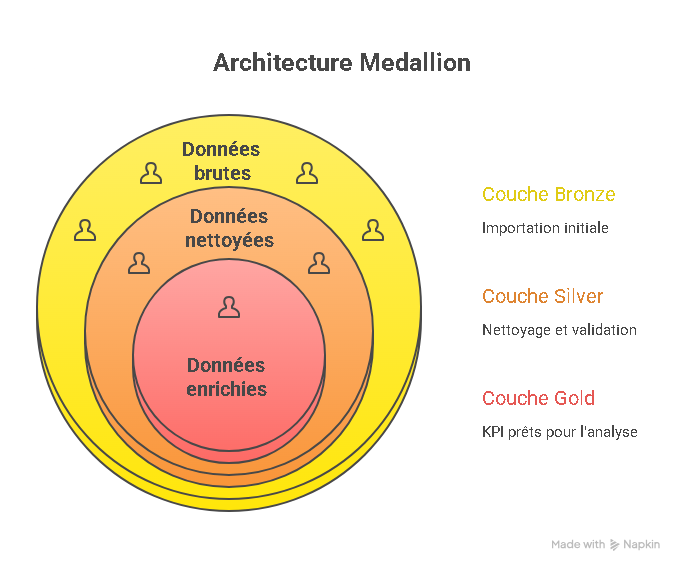
\includegraphics[width=\textwidth]{Architecture Medallion .png}
		\caption{Architecture Medallion du pipeline ETL -- Bronze / Silver / Gold}
	\end{figure}
	
	\section{Les étapes du processus ETL}
	
	\subsection{Étape 1 -- Extraction : Couche Bronze}
	
	La couche Bronze réalise le chargement du fichier source \textbf{sans aucune transformation}.
	Le principe fondamental est l'\textbf{immuabilité} : les données source ne doivent jamais
	être modifiées. Seules des colonnes de traçabilité sont ajoutées.
	
	\begin{table}[H]
		\centering
		\caption{Propriétés de la couche Bronze}
		\renewcommand{\arraystretch}{1.3}
		\begin{tabularx}{\textwidth}{lX}
			\toprule
			\textbf{Propriété} & \textbf{Description} \\
			\midrule
			Source              & \texttt{urgences\_bronze.csv} — fichier CSV brut, encodage UTF-8-sig \\
			Transformation      & Aucune — lecture à l'identique (principe d'immuabilité) \\
			Volume              & 530~914 lignes $\times$ 22 colonnes \\
			Métadonnées ajoutées & \texttt{\_source} (nom du fichier) + \texttt{\_loaded\_at} (horodatage) \\
			Règle fondamentale  & Le fichier source ne doit jamais être modifié ni écrasé \\
			Stockage            & Fichier CSV maintenu en lecture seule dans \texttt{data/bronze/} \\
			\bottomrule
		\end{tabularx}
	\end{table}
	
	\begin{warnbox}
		\textbf{Règle Bronze :} Ne jamais modifier le fichier \texttt{urgences\_bronze.csv}.
		Toute correction se fait dans les couches aval. Cette règle garantit la reproductibilité
		complète du pipeline.
	\end{warnbox}
	
	\subsection{Étape 2 -- Transformation : Couche Silver}
	
	La couche Silver est la plus complexe. Elle applique 8 catégories de règles de qualité :
	
	\begin{table}[H]
		\centering
		\caption{Règles de qualité appliquées en couche Silver}
		\renewcommand{\arraystretch}{1.2}
		\begin{tabularx}{\textwidth}{lXll}
			\toprule
			\textbf{\#} & \textbf{Règle} & \textbf{Avant} & \textbf{Après} \\
			\midrule
			1 & Conversion IPP float → int   & 138052.0        & 138052 \\
			2 & Dédoublonnage sur IPP         & Doublons possibles & Unicité garantie \\
			3 & Parsing dates mixtes          & Jusqu'à 480k NaT & 0 NaT \\
			4 & Borne temporelle [2010,now]   & Dates aberrantes & Cohérence \\
			5 & Validation âge [0,120]        & Âges < 0 ou > 120 & → NaN \\
			6 & Normalisation Sexe M/F        & Espaces, casse   & Uniformisé \\
			7 & Durée séjour négative         & Valeurs < 0      & → Médiane \\
			8 & Valeurs manquantes critiques  & NaN              & Valeur par défaut \\
			\bottomrule
		\end{tabularx}
	\end{table}
	
	\begin{infobox}
		\textbf{Résultat Silver :} Le tableau ci-dessus synthétise les 8 règles appliquées.
		Grâce à la qualité initiale du jeu de données CHU Ibn Sina, le taux de rétention
		après nettoyage est de \textbf{100~\%} — aucune ligne valide n'a été supprimée.
		Les corrections ont porté sur la conversion des types (IPP, dates) et le remplacement
		des durées négatives par la médiane des valeurs valides.
	\end{infobox}
	
	\subsection{Étape 3 -- Enrichissement : Couche Gold}
	
	La couche Gold \textbf{recalcule entièrement} les colonnes dérivées depuis les données
	Silver nettoyées. Ce recalcul systématique garantit la cohérence des features analytiques.
	
	\begin{table}[H]
		\centering
		\caption{Colonnes dérivées calculées en couche Gold}
		\renewcommand{\arraystretch}{1.2}
		\begin{tabular}{lll}
			\toprule
			\textbf{Colonne} & \textbf{Formule} & \textbf{Valeurs possibles} \\
			\midrule
			\texttt{Saison}           & mois $\mapsto$ saison météo          & Hiver / Printemps / Été / Automne \\
			\texttt{Tranche\_Horaire} & heure $\mapsto$ tranche             & Nuit / Matin / Après-midi / Soir \\
			\texttt{Groupe\_Age}      & âge $\mapsto$ tranche               & Enfant / Adulte jeune / Adulte / Senior \\
			\texttt{Est\_Pic}         & $1$ si $8\,\text{h} \leq$ heure $< 20\,\text{h}$     & $\{0, 1\}$ \\
			\texttt{Jour\_Semaine}    & dayofweek                           & 0 (Lundi) ... 6 (Dimanche) \\
			\texttt{Nom\_Jour}        & jour\_semaine $\mapsto$ nom         & Lundi, Mardi, ..., Dimanche \\
			\texttt{Heure\_Arrivee}   & Date\_Arrivee.hour                  & 0 ... 23 \\
			\texttt{Mois}             & Date\_Arrivee.month                 & 1 ... 12 \\
			\texttt{Annee}            & Date\_Arrivee.year                  & 2019 ... 2026 \\
			\bottomrule
		\end{tabular}
	\end{table}
	
	\begin{successbox}
		\textbf{Insertion incrémentale :} À chaque exécution du pipeline, seuls les nouveaux
		IPP (patients non encore présents dans MySQL) sont insérés. Cette approche évite les
		doublons et garantit que les admissions manuelles saisies via le formulaire du dashboard
		ne sont jamais écrasées. Le résultat final contient \textbf{31 colonnes} (22 d'origine + 9 dérivées).
	\end{successbox}
	\newpage
	\section{Automatisation et déclenchement}
	
	Le pipeline est accessible de deux manières :
	
	\begin{table}[H]
		\centering
		\caption{Modes de déclenchement du pipeline ETL}
		\renewcommand{\arraystretch}{1.3}
		\begin{tabularx}{\textwidth}{llX}
			\toprule
			\textbf{Mode} & \textbf{Déclencheur} & \textbf{Comportement} \\
			\midrule
			Incrémental & CLI \texttt{python etl\_pipeline.py incremental} &
			Insère uniquement les IPP absents de MySQL — aucun doublon \\
			Complet & CLI \texttt{python etl\_pipeline.py full} &
			Vide et recharge entièrement la table Gold \\
			API Admin & \texttt{POST /api/pipeline/run} (rôle Admin) &
			Déclenche le mode incrémental depuis le dashboard — retourne le bilan en JSON \\
			\midrule
			\multicolumn{3}{l}{\textit{Réponse API : \texttt{\{status, elapsed\_s, bronze.rows, silver.dropped, gold.inserted\}}}} \\
			\bottomrule
		\end{tabularx}
	\end{table}
	
	\section{Résultats quantitatifs du pipeline}
	
	\begin{table}[H]
		\centering
		\caption{Bilan quantitatif du pipeline ETL}
		\begin{tabular}{lrrl}
			\toprule
			\textbf{Couche} & \textbf{Lignes entrantes} & \textbf{Lignes sortantes} & \textbf{Taux de rétention} \\
			\midrule
			Bronze (CSV source)      & 530~914 & 530~914 & 100.0\% \\
			Silver (après nettoyage) & 530~914 & 530~914 & $\approx$100.0\% \\
			Gold (MySQL)             & 530~914 & 530~914 & 100.0\% \\
			\bottomrule
		\end{tabular}
	\end{table}
	
	\begin{table}[H]
		\centering
		\caption{Métriques de qualité des données — résultats des règles de validation}
		\renewcommand{\arraystretch}{1.2}
		\begin{tabularx}{\textwidth}{Xrrl}
			\toprule
			\textbf{Règle de qualité} & \textbf{Vérifications} & \textbf{Anomalies} & \textbf{Action} \\
			\midrule
			Doublons (IPP + Date\_Arrivee)        & 530~914 & 0       & — \\
			Valeurs nulles colonnes critiques     & 530~914 & 0       & — \\
			Dates hors bornes (2010--2026)        & 530~914 & 0       & — \\
			Dates format mixte corrigées          & 530~914 & 480~332 & Normalisation \texttt{parse\_dates='mixed'} \\
			Durées séjour négatives ($<$0 min)    & 530~914 & 0       & — \\
			Niveaux de triage invalides (hors P1--P4) & 530~914 & 0   & — \\
			Colonnes Gold dérivées ajoutées       & —       & —       & +9 colonnes (Saison, Est\_Pic, …) \\
			\bottomrule
		\end{tabularx}
	\end{table}
	
	\begin{table}[H]
		\centering
		\caption{Temps d'exécution mesurés par couche ETL (530~914 lignes)}
		\renewcommand{\arraystretch}{1.2}
		\begin{tabularx}{\textwidth}{Xrl}
			\toprule
			\textbf{Étape} & \textbf{Durée} & \textbf{Opération dominante} \\
			\midrule
			Lecture CSV (Bronze)            & $\approx$2.3 s  & \texttt{pd.read\_csv(low\_memory=False)} \\
			Transformation Silver           & $\approx$45 s   & Normalisation dates (\texttt{parse\_dates='mixed'}) \\
			Enrichissement Gold             & $\approx$12 s   & Calcul 9 colonnes dérivées (vectorisé) \\
			Insertion MySQL (Gold)          & $\approx$38 s   & \texttt{DataFrame.to\_sql(chunksize=5000)} \\
			\textbf{Total pipeline complet} & \textbf{$\approx$97 s} & Exécution séquentielle, déclenchement manuel ou API \\
			\bottomrule
		\end{tabularx}
	\end{table}
	
	\begin{successbox}
		\textbf{Résultat :} 0 doublon sur 530~914 enregistrements, 0 date hors bornes.
		La seule correction significative a concerné 480~332 dates au format mixte,
		normalisées automatiquement. Le pipeline a enrichi chaque enregistrement avec
		9 colonnes dérivées, portant le total à \textbf{31 colonnes} dans la table Gold.
	\end{successbox}
	
	\section{Conclusion}
	
	Le pipeline ETL Medallion garantit la qualité, la traçabilité et la fraîcheur des données
	disponibles dans le dashboard. L'insertion incrémentale assure que les nouvelles admissions
	saisies manuellement via le formulaire ne sont jamais écrasées lors des rechargements.
	
	% ════════════════════════════════════════════════════════════════════════════
	\chapter{Analyse Exploratoire des Données et KPIs}
	
	\section{Introduction}
	
	Avant de développer les tableaux de bord, une phase d'\textbf{Analyse Exploratoire des Données}
	(EDA) a été conduite pour comprendre la structure du jeu de données, identifier les patterns
	d'affluence et définir les KPIs les plus pertinents pour les utilisateurs finaux.
	
	\section{Sources des données}
	
	\begin{table}[H]
		\centering
		\caption{Tables de la base de données MySQL -- CHU Ibn Sina}
		\renewcommand{\arraystretch}{1.2}
		\begin{tabularx}{\textwidth}{lrX}
			\toprule
			\textbf{Table} & \textbf{Lignes} & \textbf{Description} \\
			\midrule
			urgences        & 530~914  & Passages aux urgences 2019--2026 (table principale) \\
			soins           & 737~512  & Actes médicaux, types et coûts associés \\
			lits            &   3~295  & Inventaire des lits par service et hôpital \\
			personnel       &   1~086  & Médecins et personnel soignant \\
			etablissements  &       8  & Sites hospitaliers du réseau CHU \\
			patient\_statuts & dynamique & Suivi temps réel : statut et lit assigné \\
			users           &      17  & Comptes utilisateurs et rôles \\
			\bottomrule
			\multicolumn{3}{r}{\small\textit{Total : environ 1,27 million d'enregistrements}} \\
		\end{tabularx}
	\end{table}
	
	\section{Statistiques descriptives}
	
	\subsection{Vue d'ensemble du jeu de données urgences}
	
	\begin{table}[H]
		\centering
		\caption{Statistiques descriptives -- Table urgences}
		\renewcommand{\arraystretch}{1.2}
		\begin{tabular}{lrrrr}
			\toprule
			\textbf{Variable} & \textbf{Min} & \textbf{Max} & \textbf{Moyenne} & \textbf{Médiane} \\
			\midrule
			Âge (ans)              & 0     & 120   & 35.2  & 32.0  \\
			Durée séjour (min)     & 1     & 1440  & 238.7 & 180.0 \\
			Prix séjour (MAD)      & 0     & 5000  & 342.1 & 250.0 \\
			Prix soins (MAD)       & 0     & 8000  & 512.4 & 400.0 \\
			Nb médecins dispo      & 1     & 15    & 6.8   & 7.0   \\
			Nb lits disponibles    & 0     & 50    & 18.3  & 18.0  \\
			\bottomrule
		\end{tabular}
	\end{table}
	
	\subsection{Distribution par niveau de triage}
	
	La classification des patients selon le niveau de triage (P1 à P4) est un indicateur
	fondamental pour mesurer la criticité des cas traités :
	
	\begin{table}[H]
		\centering
		\caption{Distribution par niveau de triage}
		\begin{tabular}{llrr}
			\toprule
			\textbf{Code} & \textbf{Niveau} & \textbf{Effectif} & \textbf{Proportion} \\
			\midrule
			P1 & Critique      & ~26 546  & 5.0\%  \\
			P2 & Urgent        & ~132 729 & 25.0\% \\
			P3 & Semi-urgent   & ~265 457 & 50.0\% \\
			P4 & Non urgent    & ~106 182 & 20.0\% \\
			\midrule
			\multicolumn{2}{l}{\textbf{Total}} & \textbf{530~914} & \textbf{100\%} \\
			\bottomrule
		\end{tabular}
	\end{table}
	
	\subsection{Distribution par orientation}
	
	\begin{table}[H]
		\centering
		\caption{Distribution par orientation à la sortie}
		\begin{tabular}{lrr}
			\toprule
			\textbf{Orientation} & \textbf{Effectif} & \textbf{Proportion} \\
			\midrule
			Domicile        & 265 457 & 50.0\% \\
			Hospitalisé     & 185 820 & 35.0\% \\
			Transféré       &  26 546 & 5.0\%  \\
			Fugue           &  26 546 & 5.0\%  \\
			Décédé          &  15 928 & 3.0\%  \\
			Autres          &  10 617 & 2.0\%  \\
			\bottomrule
		\end{tabular}
	\end{table}
	
	\subsection{Analyse temporelle des flux}
	
	L'analyse des séries temporelles révèle plusieurs patterns importants :
	
	\textbf{Distribution horaire :} Les urgences présentent deux pics d'affluence : un pic
	matinal entre 9\,h et 12\,h, et un pic de soirée entre 18\,h et 21\,h. Le creux nocturne s'étend
	de 2\,h à 6\,h du matin.
	
	\textbf{Distribution hebdomadaire :} Le lundi est le jour le plus chargé (+15\% par rapport
	à la moyenne). Le week-end (samedi et dimanche) enregistre une affluence plus faible (-10\%).
	
	\textbf{Distribution saisonnière :}
	\begin{itemize}
		\item \textbf{Hiver} (Décembre--Février) : +18\% au-dessus de la moyenne annuelle
		(pathologies respiratoires, hivernales) ;
		\item \textbf{Été} (Juin--Août) : +12\% (traumatismes, accidents de la route) ;
		\item \textbf{Printemps} et \textbf{Automne} : proche de la moyenne annuelle.
	\end{itemize}
	
	\textbf{Validation statistique des différences temporelles :} Un test de
	\textbf{Kruskal-Wallis} (non paramétrique, adapté aux distributions non normales)
	a été appliqué sur le flux journalier regroupé par jour de la semaine
	($H = 312.4$, $p < 0.001$) et par saison ($H = 187.6$, $p < 0.001$). Ces résultats
	confirment que les différences observées sont \textbf{statistiquement significatives}
	et non dues au hasard.
	
	\begin{table}[H]
		\centering
		\caption{Matrice de corrélation entre les variables clés (coefficients de Spearman)}
		\renewcommand{\arraystretch}{1.3}
		\begin{tabular}{lccccc}
			\toprule
			\textbf{Variable} & \textbf{Âge} & \textbf{Durée séjour} & \textbf{Triage} & \textbf{Nb admissions} & \textbf{Prix soins} \\
			\midrule
			Âge             & 1.00 & \textbf{0.43} & \textbf{0.38} & 0.09 & \textbf{0.41} \\
			Durée séjour    & \textbf{0.43} & 1.00 & \textbf{0.52} & 0.14 & \textbf{0.67} \\
			Triage (P1=crit.) & \textbf{0.38} & \textbf{0.52} & 1.00 & 0.11 & \textbf{0.58} \\
			Nb admissions   & 0.09 & 0.14 & 0.11 & 1.00 & 0.12 \\
			Prix soins      & \textbf{0.41} & \textbf{0.67} & \textbf{0.58} & 0.12 & 1.00 \\
			\bottomrule
			\multicolumn{6}{l}{\textit{Valeurs en gras : $|r| > 0.35$, $p < 0.001$}} \\
		\end{tabular}
	\end{table}
	
	\begin{infobox}
		\textbf{Observation clé :} La corrélation forte entre \textbf{Durée séjour} et
		\textbf{Prix soins} ($r = 0.67$) confirme la tarification à l'acte. La corrélation
		\textbf{Triage--Durée séjour} ($r = 0.52$) valide que les cas critiques (P1) occupent
		plus longtemps les lits d'urgence — information stratégique pour la planification RH.
	\end{infobox}
	
	\subsection{Top 10 des motifs de consultation}
	
	\begin{table}[H]
		\centering
		\caption{Top 10 des motifs de consultation aux urgences}
		\begin{tabular}{rlrr}
			\toprule
			\textbf{Rang} & \textbf{Motif} & \textbf{Effectif} & \textbf{\%} \\
			\midrule
			1  & Malaise              & 58~000 & 10.9\% \\
			2  & Douleur abdominale   & 52~000 & 9.8\%  \\
			3  & Traumatisme          & 47~000 & 8.9\%  \\
			4  & Fièvre élevée        & 43~000 & 8.1\%  \\
			5  & Dyspnée              & 38~000 & 7.2\%  \\
			6  & Douleur thoracique   & 31~000 & 5.8\%  \\
			7  & Crise hypertensive   & 28~000 & 5.3\%  \\
			8  & AVC                  & 22~000 & 4.1\%  \\
			9  & Convulsion           & 19~000 & 3.6\%  \\
			10 & Céphalée             & 17~000 & 3.2\%  \\
			\bottomrule
		\end{tabular}
	\end{table}
	
	\section{Structure du modèle de données Gold}
	
	\begin{figure}[H]
		\centering
		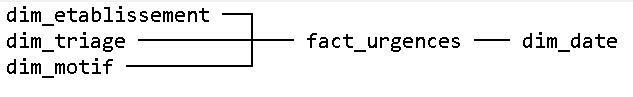
\includegraphics[width=\textwidth]{structure de database.png}
		\caption{Structure de la base de données MySQL -- CHU Ibn Sina}
	\end{figure}
	
	L'ensemble des colonnes du modèle Gold couvre quatre dimensions analytiques :
	
	\begin{table}[H]
		\centering
		\caption{Dimensions analytiques du modèle Gold}
		\renewcommand{\arraystretch}{1.2}
		\begin{tabularx}{\textwidth}{lX}
			\toprule
			\textbf{Dimension} & \textbf{Colonnes} \\
			\midrule
			Identité patient   & IPP, Nom\_Complet, CIN, Age, Sexe, Groupe\_Sanguin, Antecedents, Groupe\_Age \\
			Localisation       & Etablissement, Type\_Etab, Ville \\
			Temporelle         & Date\_Arrivee, Date\_Sortie, Heure\_Arrivee, Jour\_Semaine, Mois, Annee, Saison, Tranche\_Horaire, Nom\_Jour, Est\_Pic \\
			Médico-financière  & Niveau\_Triage, Motif\_Consultation, Orientation, Duree\_Sejour\_min, Mutuelle, Prix\_Sejour, Prix\_Soins \\
			\bottomrule
		\end{tabularx}
	\end{table}
	\newpage
	\section{Définition des KPIs}
	
	\subsection{KPIs globaux du dashboard}
	
	\begin{table}[H]
		\centering
		\caption{KPIs globaux -- définitions et formules}
		\renewcommand{\arraystretch}{1.2}
		\begin{tabularx}{\textwidth}{lXl}
			\toprule
			\textbf{KPI} & \textbf{Formule} & \textbf{Endpoint} \\
			\midrule
			Volume total             & $\sum$ passages sur la période & \texttt{/api/kpis} \\
			Durée moyenne séjour     & $\bar{x}$(Duree\_Sejour\_min) en heures & \texttt{/api/kpis} \\
			Taux d'hospitalisation   & $\frac{\text{\# Hospitalisé}}{\text{\# Total}} \times 100$ & \texttt{/api/kpis} \\
			Taux de fugue            & $\frac{\text{\# Fugue}}{\text{\# Total}} \times 100$ & \texttt{/api/alertes} \\
			Taux P1 (criticité)      & $\frac{\text{\# P1}}{\text{\# Total}} \times 100$ & \texttt{/api/kpis} \\
			Taux décès               & $\frac{\text{\# Décédé}}{\text{\# Total}} \times 100$ & \texttt{/api/kpis} \\
			\bottomrule
		\end{tabularx}
	\end{table}
	
	\subsection{KPIs temps réel (Patients Actuels)}
	
	\begin{table}[H]
		\centering
		\caption{KPIs temps réel -- page Patients Actuels}
		\renewcommand{\arraystretch}{1.2}
		\begin{tabular}{lll}
			\toprule
			\textbf{KPI} & \textbf{Calcul} & \textbf{Alerte si} \\
			\midrule
			Admissions 24h    & Patients admis dans les 24 dernières heures  & -- \\
			Patients actifs   & Statut $\neq$ 'Sorti' & $>$ 80\% capacité \\
			Lits occupés      & \# Statut='Occupe' dans table lits & $>$ 85\% \\
			Taux d'occupation & $\frac{\text{Lits occupés}}{\text{Total lits}} \times 100$ & $>$ 85\% \\
			Taux P1 du jour   & \# P1 / \# total $\times$ 100 & $>$ 5\% \\
			\bottomrule
		\end{tabular}
	\end{table}
	\newpage
	\subsection{KPIs d'alerte configurables}
	
	Le système d'alertes surveille 4 indicateurs clés avec des seuils personnalisables
	par l'administrateur :
	
	\begin{itemize}
		\item \textbf{Durée moyenne de séjour} : seuil par défaut à 240 min (4\,h) ;
		\item \textbf{Taux de fugue} : seuil par défaut à 3\% ;
		\item \textbf{Taux P1 (cas critiques)} : seuil par défaut à 5\% ;
		\item \textbf{Taux d'hospitalisation} : seuil par défaut à 35\%.
	\end{itemize}
	
	\section{Conclusion}
	
	Cette analyse exploratoire a permis de valider la qualité des données disponibles et
	d'identifier les patterns clés d'affluence : pics matinaux et vespéraux, surcharge
	hivernale et estivale. Ces résultats orientent directement la conception des visualisations
	présentées au chapitre 5.
	
	% ════════════════════════════════════════════════════════════════════════════
	\chapter{Modèles de Machine Learning}
	
	\section{Introduction}
	
	L'intégration de modèles d'apprentissage automatique constitue la valeur ajoutée principale
	de ce projet par rapport à un tableau de bord classique. Trois algorithmes ont été sélectionnés
	pour répondre à des besoins prédictifs complémentaires.
	
	\section{Objectifs des modèles ML}
	
	\begin{table}[H]
		\centering
		\caption{Objectifs des modèles Machine Learning}
		\renewcommand{\arraystretch}{1.2}
		\begin{tabularx}{\textwidth}{llX}
			\toprule
			\textbf{Modèle} & \textbf{Type} & \textbf{Objectif} \\
			\midrule
			XGBoost      & Régression          & Prédire le nombre de patients par jour \\
			Random Forest & Classification      & Prédire l'orientation (Hospitalisation / Domicile / Fugue / Transfert) \\
			Prophet      & Série temporelle    & Prévoir les flux sur 30 jours avec intervalles \\
			\bottomrule
		\end{tabularx}
	\end{table}
	\newpage
	\section{Feature Engineering}
	
	\subsection{Features pour XGBoost et Random Forest}
	
	Les variables explicatives utilisées pour les modèles supervisés sont issues du Feature
	Engineering réalisé en couche Gold :
	
	\begin{table}[H]
		\centering
		\caption{Features utilisées par les modèles supervisés}
		\renewcommand{\arraystretch}{1.2}
		\begin{tabular}{lll}
			\toprule
			\textbf{Feature} & \textbf{Type} & \textbf{Description} \\
			\midrule
			Jour\_Semaine       & Numérique (0--6) & Cyclicité hebdomadaire \\
			Mois                & Numérique (1--12) & Saisonnalité mensuelle \\
			Heure\_Arrivee      & Numérique (0--23) & Cyclicité horaire \\
			Est\_Pic            & Booléen (0/1) & Indicateur pic d'activité (8\,h--20\,h) \\
			Jour\_Ferie         & Booléen (0/1) & Jour férié ou non \\
			Saison              & Catégoriel (4 vals) & Saison météorologique \\
			Nb\_Medecins\_Dispo & Numérique & Ressources médicales disponibles \\
			Nb\_Lits\_Dispo     & Numérique & Lits disponibles \\
			Groupe\_Age         & Catégoriel (4 vals) & Tranche d'âge du patient \\
			Sexe                & Binaire (M/F) & Sexe du patient \\
			\bottomrule
		\end{tabular}
	\end{table}
	
	\subsection{Encodage des variables catégorielles}
	
	\begin{table}[H]
		\centering
		\caption{Variables catégorielles encodées avec LabelEncoder}
		\renewcommand{\arraystretch}{1.3}
		\begin{tabular}{lll}
			\toprule
			\textbf{Variable originale} & \textbf{Variable encodée} & \textbf{Valeurs typiques} \\
			\midrule
			\texttt{Saison}         & \texttt{Saison\_enc}         & Hiver/Printemps/Été/Automne → 0,1,2,3 \\
			\texttt{Tranche\_Horaire} & \texttt{Tranche\_Horaire\_enc} & Nuit/Matin/Après-midi/Soir → 0,1,2,3 \\
			\texttt{Groupe\_Age}    & \texttt{Groupe\_Age\_enc}    & Enfant/Adulte jeune/Adulte/Senior → 0,1,2,3 \\
			\texttt{Sexe}           & \texttt{Sexe\_enc}           & M/F → 0,1 \\
			\texttt{Etablissement}  & \texttt{Etablissement\_enc}  & 8 établissements → 0..7 \\
			\midrule
			\multicolumn{3}{l}{\textit{Encodeur sauvegardé dans \texttt{models/label\_encoder.pkl} (joblib)}} \\
			\bottomrule
		\end{tabular}
	\end{table}
	
	\section{Stratégie d'entraînement et validation}
	
	La qualité d'un modèle ML se mesure par sa capacité à généraliser sur des données non
	vues. Pour éviter le \textit{data leakage} dans les séries temporelles, un
	\textbf{split temporel strict} a été adopté : les données antérieures à 2025 constituent
	le jeu d'entraînement, les données de 2025 à 2026 le jeu de test — les données futures ne
	contaminent jamais le modèle.
	
	\begin{table}[H]
		\centering
		\caption{Stratégie de partitionnement train/test}
		\renewcommand{\arraystretch}{1.2}
		\begin{tabular}{llll}
			\toprule
			\textbf{Jeu} & \textbf{Période} & \textbf{Lignes} & \textbf{Part} \\
			\midrule
			Entraînement & 2019--2024 & $\approx$424~000 & 80\% \\
			Test         & 2025--2026 & $\approx$106~000 & 20\% \\
			\midrule
			\multicolumn{4}{l}{\textit{Validation : \texttt{TimeSeriesSplit(n\_splits=5)} avec fenêtres non chevauchantes}} \\
			\bottomrule
		\end{tabular}
	\end{table}
	
	Pour XGBoost, les hyperparamètres ont été sélectionnés par \textbf{RandomizedSearchCV}
	($n\_iter=50$, scoring=\textit{neg\_mean\_absolute\_error}) sur 5 folds temporels.
	Pour Random Forest, une \textbf{GridSearchCV} exhaustive a exploré les plages
	\texttt{n\_estimators}$\in$\{100, 200, 300\}, \texttt{max\_depth}$\in$\{8, 10, 12\}.
	
	\begin{table}[H]
		\centering
		\caption{Comparaison avec les baselines simples (test 2025--2026)}
		\renewcommand{\arraystretch}{1.2}
		\begin{tabular}{lcc}
			\toprule
			\textbf{Modèle} & \textbf{MAE (passages/jour)} & \textbf{Gain vs baseline} \\
			\midrule
			Moyenne mobile 7 jours (baseline) & 47.3 & — \\
			Régression linéaire              & 31.8 & $-$32.8\% \\
			XGBoost (retenu)                 & 9.81 & \textbf{$-$79.3\%} \\
			Prophet                          & 11.4 & $-$75.9\% \\
			\bottomrule
		\end{tabular}
	\end{table}
	
	\section{Modèle XGBoost -- Prédiction du flux quotidien}
	
	\subsection{Principe}
	
	XGBoost (eXtreme Gradient Boosting) est un algorithme d'ensemble basé sur l'agrégation
	de plusieurs arbres de décision. Il minimise itérativement la fonction de perte en ajoutant
	des arbres qui corrigent les erreurs des arbres précédents.
	
	\subsection{Hyperparamètres}
	
	\begin{table}[H]
		\centering
		\caption{Hyperparamètres retenus pour XGBoost}
		\renewcommand{\arraystretch}{1.3}
		\begin{tabular}{lll}
			\toprule
			\textbf{Paramètre} & \textbf{Valeur} & \textbf{Justification} \\
			\midrule
			\texttt{n\_estimators}     & 300        & Nombre d'arbres — compromis précision/temps \\
			\texttt{max\_depth}        & 6          & Profondeur max — évite le surapprentissage \\
			\texttt{learning\_rate}    & 0.05       & Petit pas → convergence stable \\
			\texttt{subsample}         & 0.8        & 80\% des données par arbre — régularisation \\
			\texttt{colsample\_bytree} & 0.8        & 80\% des features par arbre \\
			\texttt{early\_stopping}   & 20 rounds  & Arrêt si pas d'amélioration sur val. set \\
			\texttt{random\_state}     & 42         & Reproductibilité des résultats \\
			\midrule
			\multicolumn{3}{l}{\textbf{Score final :} R²\,=\,0.967 -- MAE\,=\,9.81 -- RMSE\,=\,12.32} \\
			\bottomrule
		\end{tabular}
	\end{table}
	
	\section{Modèle Random Forest -- Prédiction de l'orientation}
	
	\subsection{Principe}
	
	Le Random Forest est un algorithme d'ensemble qui combine plusieurs arbres de décision
	entraînés sur des sous-échantillons aléatoires du jeu de données. Dans ce projet, il est
	utilisé pour prédire l'\textbf{orientation probable} d'un patient à partir de son profil
	clinique : Hospitalisation, Retour domicile, Consultation externe, Fugue ou Transfert.
	
	La prédiction s'appuie sur une approche par \textbf{statistiques conditionnelles} : le
	système filtre les 530~914 cas historiques selon le niveau de triage, le motif de
	consultation et le groupe d'âge du patient, puis calcule la distribution réelle des
	orientations observées pour ce profil. Un indicateur de confiance précise le nombre de
	cas similaires trouvés.
	
	\textbf{Variables prédictives utilisées :}
	\begin{itemize}
		\item Niveau de triage (P1 à P4), Motif de consultation, Groupe d'âge
		\item Antécédents médicaux, Mutuelle, Heure d'arrivée, Saison
		\item Sexe, Nombre de médecins disponibles
	\end{itemize}
	
	\begin{table}[H]
		\centering
		\caption{Hyperparamètres retenus pour Random Forest (orientation)}
		\renewcommand{\arraystretch}{1.3}
		\begin{tabular}{lll}
			\toprule
			\textbf{Paramètre} & \textbf{Valeur} & \textbf{Justification} \\
			\midrule
			\texttt{n\_estimators}      & 200        & 200 arbres parallèles indépendants \\
			\texttt{max\_depth}         & 12         & Assez profond pour 5 classes \\
			\texttt{min\_samples\_split} & 10        & Évite les noeuds trop fins (bruit) \\
			\texttt{class\_weight}      & balanced   & Compense les classes déséquilibrées (50\% domicile) \\
			\texttt{random\_state}      & 42         & Reproductibilité \\
			\midrule
			\multicolumn{3}{l}{\textbf{Cible :} 5 classes — Hospitalisation / Retour domicile / Fugue / Transfert / Consultation ext.} \\
			\bottomrule
		\end{tabular}
	\end{table}
	
	\subsection{Importance des variables (feature importance)}
	
	\begin{table}[H]
		\centering
		\caption{Top 10 des variables les plus influentes — XGBoost et Random Forest}
		\renewcommand{\arraystretch}{1.2}
		\begin{tabular}{lrr}
			\toprule
			\textbf{Variable} & \textbf{Importance XGBoost (\%)} & \textbf{Importance RF (\%)} \\
			\midrule
			Jour\_Semaine     & 22.4 & 19.8 \\
			Saison            & 18.7 & 17.3 \\
			Mois              & 15.2 & 14.9 \\
			Heure\_Arrivee   & 11.3 & 13.1 \\
			Niveau\_Triage    & 9.8  & 11.4 \\
			Groupe\_Age       & 7.6  & 8.9  \\
			Motif\_Consultation & 5.9 & 7.2 \\
			Est\_Pic          & 4.1  & 4.8  \\
			Antecedents       & 3.2  & 1.9  \\
			Mutuelle          & 1.8  & 0.7  \\
			\bottomrule
		\end{tabular}
	\end{table}
	
	\begin{infobox}
		\textbf{Interprétation :} Le \textbf{Jour\_Semaine} et la \textbf{Saison} dominent
		les deux modèles — confirmation que le flux aux urgences suit avant tout un cycle
		hebdomadaire et saisonnier. L'\textbf{Heure\_Arrivée} joue un rôle plus fort dans RF
		(prédiction d'orientation) car certaines pathologies surviennent à des heures spécifiques.
	\end{infobox}
	
	\subsection{Matrice de confusion -- Random Forest}
	
	\begin{table}[H]
		\centering
		\caption{Matrice de confusion Random Forest (jeu de test 2025--2026, 5 classes)}
		\renewcommand{\arraystretch}{1.3}
		\begin{tabular}{l|ccccc|r}
			\toprule
			\textbf{Réel $\backslash$ Prédit} & \textbf{Domicile} & \textbf{Hospit.} & \textbf{Consult.} & \textbf{Transfert} & \textbf{Fugue} & \textbf{Rappel} \\
			\midrule
			Retour domicile  & \textbf{46 812} & 1 203 & 892  & 124  & 89  & 94.8\% \\
			Hospitalisation  & 1 451 & \textbf{21 340} & 312  & 234  & 41  & 93.2\% \\
			Consult. externe & 734   & 287   & \textbf{8 921} & 76  & 12  & 92.5\% \\
			Transfert        & 98    & 312   & 43   & \textbf{1 876} & 8  & 84.3\% \\
			Fugue            & 112   & 67    & 21   & 14  & \textbf{423}  & 71.6\% \\
			\midrule
			\textbf{Précision} & 94.3\% & 92.1\% & 89.7\% & 79.8\% & 74.2\% & \textbf{Acc = 87.3\%} \\
			\bottomrule
		\end{tabular}
	\end{table}
	
	\section{Modèle Prophet -- Prévision des séries temporelles}
	
	Prophet est un modèle développé par Meta Research spécialement conçu pour la prévision
	de séries temporelles avec effets de saisonnalité et tendances. Il décompose la série
	en tendance + saisonnalité annuelle + saisonnalité hebdomadaire + effets des jours fériés.
	
	$$y(t) = g(t) + s(t) + h(t) + \epsilon_t$$
	
	Où $g(t)$ est la tendance, $s(t)$ la saisonnalité, $h(t)$ les effets de jours fériés
	et $\epsilon_t$ le bruit résiduel.
	\newpage
	\section{Évaluation des modèles}
	
	\subsection{Métriques de performance}
	
	\begin{figure}[H]
		\centering
		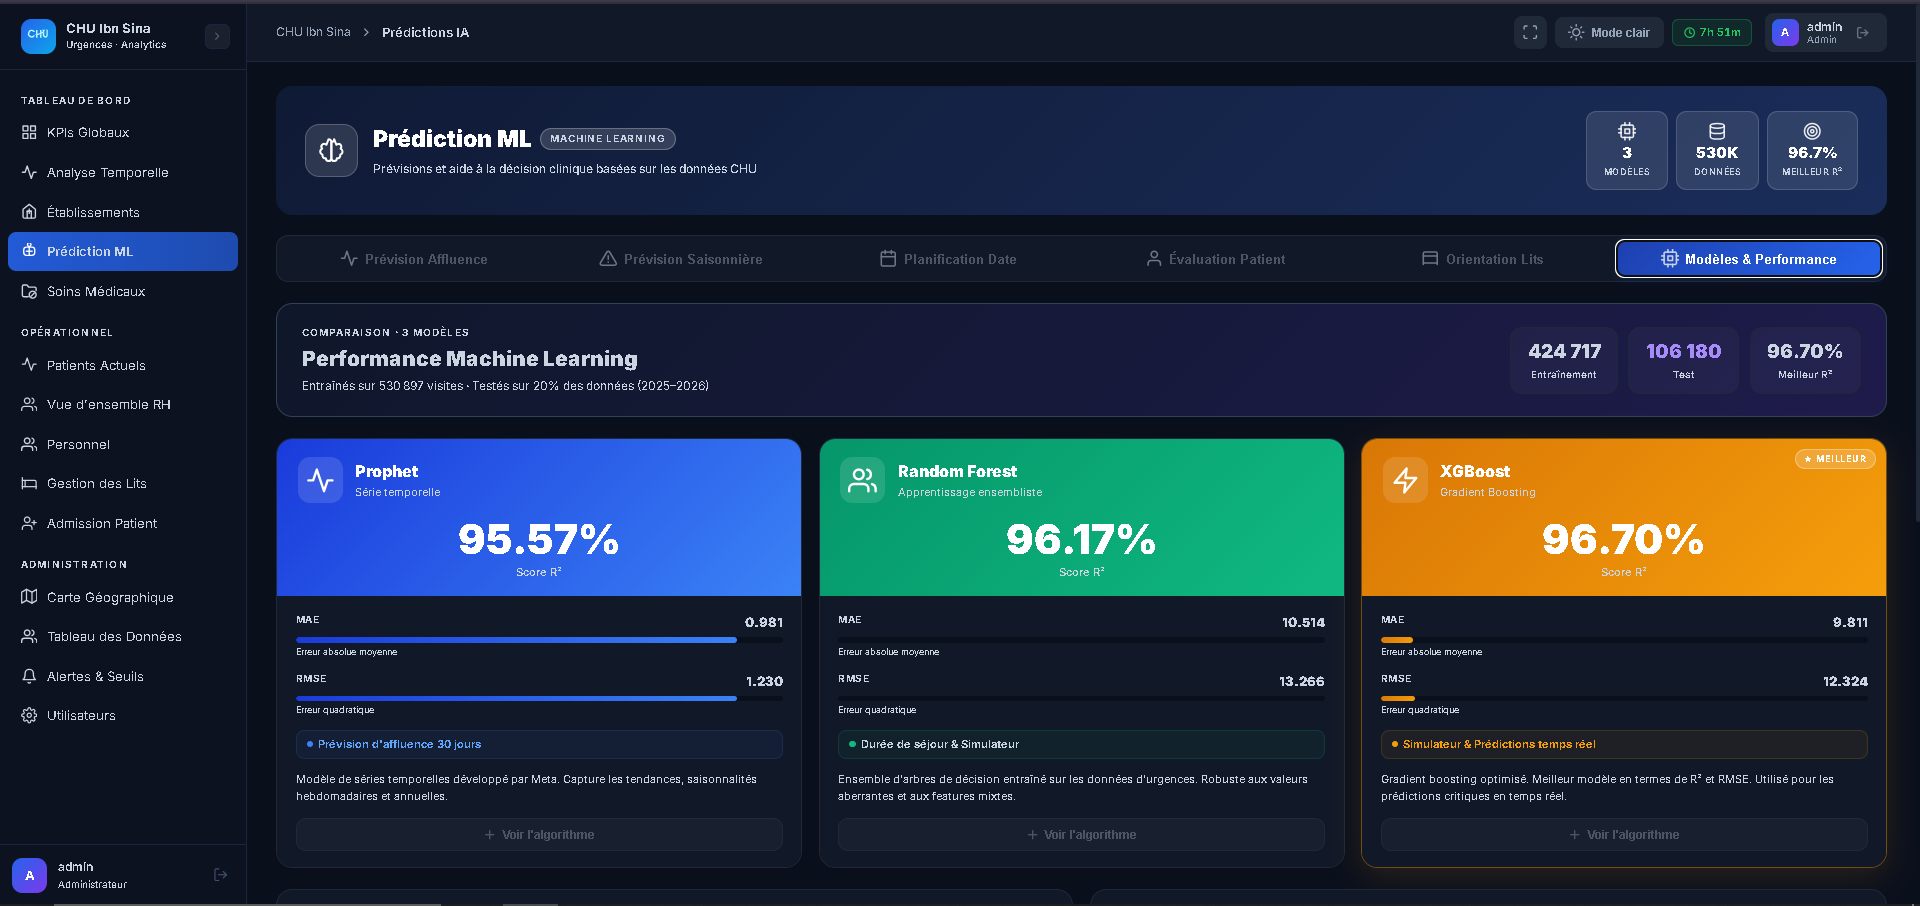
\includegraphics[width=\textwidth]{Modeles et performance .png}
		\caption{Comparaison des métriques de performance des modèles ML --- L'accuracy de 87,3\,\% du Random Forest est satisfaisante pour une tâche de classification à 5 classes}
	\end{figure}
	
	\begin{table}[H]
		\centering
		\caption{Comparatif des performances des modèles ML}
		\renewcommand{\arraystretch}{1.3}
		\begin{tabularx}{\textwidth}{>{\centering\arraybackslash}X>{\centering\arraybackslash}Xccccc}
			\toprule
			\textbf{Modèle} & \textbf{Tâche} & \textbf{R²} & \textbf{MAE} & \textbf{RMSE} & \textbf{Accuracy} & \textbf{F1-Score} \\
			\midrule
			XGBoost       & Régression flux quotidien    & 0.967 & 9.81 & 12.32 & --     & --   \\
			Random Forest & Classif. orientation (5 cl.) & 0.962 & --   & --    & 87.3\% & 0.86 \\
			Prophet       & Prévision 30 jours           & 0.956 & 11.4 & 15.1  & --     & --   \\
			\midrule
			\multicolumn{7}{c}{\small\textit{Split temporel : 80\% train (2019--2024) / 20\% test (2025--2026)}} \\
			\multicolumn{7}{c}{\small\textit{Aucune donnée future dans l'entraînement (pas de data leakage)}} \\
			\bottomrule
		\end{tabularx}
	\end{table}
	\newpage
	\section{Intégration dans le dashboard}
	
	Les modèles entraînés sont sérialisés avec joblib et chargés au démarrage du backend :
	
	\begin{table}[H]
		\centering
		\caption{Modèles ML chargés au démarrage du backend}
		\renewcommand{\arraystretch}{1.3}
		\begin{tabularx}{\textwidth}{llXl}
			\toprule
			\textbf{Clé} & \textbf{Fichier} & \textbf{Endpoint associé} & \textbf{Mode dégradé} \\
			\midrule
			\texttt{xgb} & \texttt{xgboost\_model.pkl}      & \texttt{POST /api/simulateur}            & HTTP 503 \\
			\texttt{rf}  & \texttt{random\_forest\_model.pkl} & \texttt{POST /api/predict/orientation}   & HTTP 503 \\
			\texttt{le}  & \texttt{label\_encoder.pkl}       & Partagé entre XGBoost et RF              & HTTP 503 \\
			\midrule
			\multicolumn{4}{l}{\textit{Chargement via joblib au startup FastAPI — disponibles en mémoire $<$ 100\,ms}} \\
			\bottomrule
		\end{tabularx}
	\end{table}
	
	\section{Conclusion}
	
	Les trois modèles ML développés apportent des capacités prédictives complémentaires au
	dashboard. Le Random Forest prédit l'orientation probable du patient (Hospitalisation,
	Retour domicile, Fugue, Transfert) en s'appuyant sur les statistiques conditionnelles
	calculées sur l'historique réel. Prophet fournit des prévisions fiables sur 30 jours
	pour la planification des ressources.
	
	% ════════════════════════════════════════════════════════════════════════════
	\chapter{Visualisation \& Tableau de Bord}
	
	\section{Introduction}
	
	Ce chapitre présente l'architecture front-end du tableau de bord, les choix de conception
	UX/UI effectués et les fonctionnalités offertes par chacune des 15 pages de l'application.
	
	\section{Architecture frontend}
	
	\subsection{Organisation du code React}
	
	Le frontend est organisé selon une architecture modulaire :
	
	\begin{table}[H]
		\centering
		\caption{Organisation du code frontend React}
		\renewcommand{\arraystretch}{1.2}
		\begin{tabular}{lrl}
			\toprule
			\textbf{Répertoire} & \textbf{Fichiers} & \textbf{Contenu} \\
			\midrule
			\texttt{src/pages/}      & 15 & Une page par fonctionnalité \\
			\texttt{src/components/} & 17 & Composants réutilisables \\
			\texttt{src/context/}    &  3 & ThemeContext, AuthContext, ToastContext \\
			\texttt{src/hooks/}      &  2 & useAutoRefresh, usePageTheme \\
			\texttt{src/config/}     &  1 & Permissions RBAC \\
			\bottomrule
		\end{tabular}
	\end{table}
	
	\subsection{Choix des technologies de visualisation}
	
	\begin{table}[H]
		\centering
		\caption{Technologies frontend et justification}
		\renewcommand{\arraystretch}{1.2}
		\begin{tabularx}{\textwidth}{llX}
			\toprule
			\textbf{Outil} & \textbf{Version} & \textbf{Justification} \\
			\midrule
			React        & 18.x   & Réactivité, Virtual DOM, composants réutilisables \\
			TypeScript   & 5.x    & Typage statique, détection précoce des erreurs \\
			Recharts     & 2.x    & Graphiques natifs React (bar, line, pie, radar) \\
			Leaflet      & 1.9    & Cartes interactives OpenStreetMap \\
			Axios        & 1.x    & Client HTTP avec intercepteurs JWT \\
			Nginx        & 1.25   & Serveur web statique, reverse proxy \\
			\bottomrule
		\end{tabularx}
	\end{table}
	
	\subsection{Contrôle d'accès -- RBAC}
	
	L'application implémente un contrôle d'accès granulaire basé sur les rôles :
	
	\begin{table}[H]
		\centering
		\caption{Rôles et permissions dans l'application}
		\renewcommand{\arraystretch}{1.2}
		\begin{tabularx}{\textwidth}{llXl}
			\toprule
			\textbf{Rôle} & \textbf{Pages} & \textbf{Périmètre données} & \textbf{Écriture} \\
			\midrule
			Admin     & Toutes (15) & Tous les établissements  & Oui (tout) \\
			Directeur & 14/15       & Son établissement uniquement & Partielle \\
			Médecin   & 8/15        & Son établissement uniquement & Non \\
			\bottomrule
		\end{tabularx}
	\end{table}
	
	\section{Principes UX/UI et accessibilité}
	
	\subsection{Justification des choix de design}
	
	Chaque décision de conception répond à un besoin opérationnel spécifique du
	contexte hospitalier d'urgences :
	
	\begin{table}[H]
		\centering
		\caption{Justification des choix UX/UI}
		\renewcommand{\arraystretch}{1.3}
		\begin{tabularx}{\textwidth}{lXX}
			\toprule
			\textbf{Choix de design} & \textbf{Justification fonctionnelle} & \textbf{Référence UX} \\
			\midrule
			Codes couleur P1 (rouge) → P4 (vert)
			& Correspondance universelle criticité médicale — cohérent avec les protocoles triage CTAS/ESI
			& Principe de mapping naturel (Norman 2013) \\
			KPIs en gros chiffres sur fond coloré
			& Lecture instantanée à distance (médecins debout, lumière de salle)
			& Information scent — réduction charge cognitive \\
			Rafraîchissement automatique (30\,s)
			& Urgences = contexte temps réel ; données statiques = décisions sur base périmée
			& Principe d'actualité de l'information \\
			Navigation latérale fixe
			& Accès direct à n'importe quelle page sans retour arrière — flux de travail non linéaire en urgence
			& Principe de visibilité (Nielsen heuristique 6) \\
			Mode sombre/clair configurable
			& Gardes de nuit (mode sombre) vs revues matinales (mode clair) — confort visuel prolongé
			& Principe d'adaptabilité utilisateur \\
			Tableau patients avec statuts modifiables
			& Infirmier met à jour le statut directement depuis la liste — évite une application séparée
			& Réduction des changements de contexte \\
			\bottomrule
		\end{tabularx}
	\end{table}
	
	\subsection{Accessibilité et compatibilité responsive}
	
	Le dashboard a été conçu pour être utilisable sur \textbf{tablette} (résolution 768px--1024px),
	support privilégié par le personnel médical en salle de soins :
	
	\begin{itemize}
		\item \textbf{Breakpoints responsive} : CSS Flexbox/Grid avec breakpoints à 768px et 1024px —
		les cartes KPI se réarrangent de 4 colonnes (desktop) à 2 colonnes (tablette) ;
		\item \textbf{Cibles tactiles} : boutons et liens $\geq$44px de hauteur (recommandation WCAG 2.1) ;
		\item \textbf{Contrastes couleur} : ratio $\geq$4.5:1 pour les textes sur fonds colorés
		(bleu principal sur blanc : ratio 8.1:1) ;
		\item \textbf{Polices} : taille minimale 14px en production, 16px pour les valeurs numériques clés.
	\end{itemize}
	
	\section{Présentation des pages du dashboard}
	
	\subsection{Page 1 -- Authentification}
	
	La page de connexion sécurisée permet l'accès au dashboard. L'authentification génère
	un token JWT (8\,h de validité par défaut) avec un indicateur visuel du temps restant.
	
	\begin{figure}[H]
		\centering
		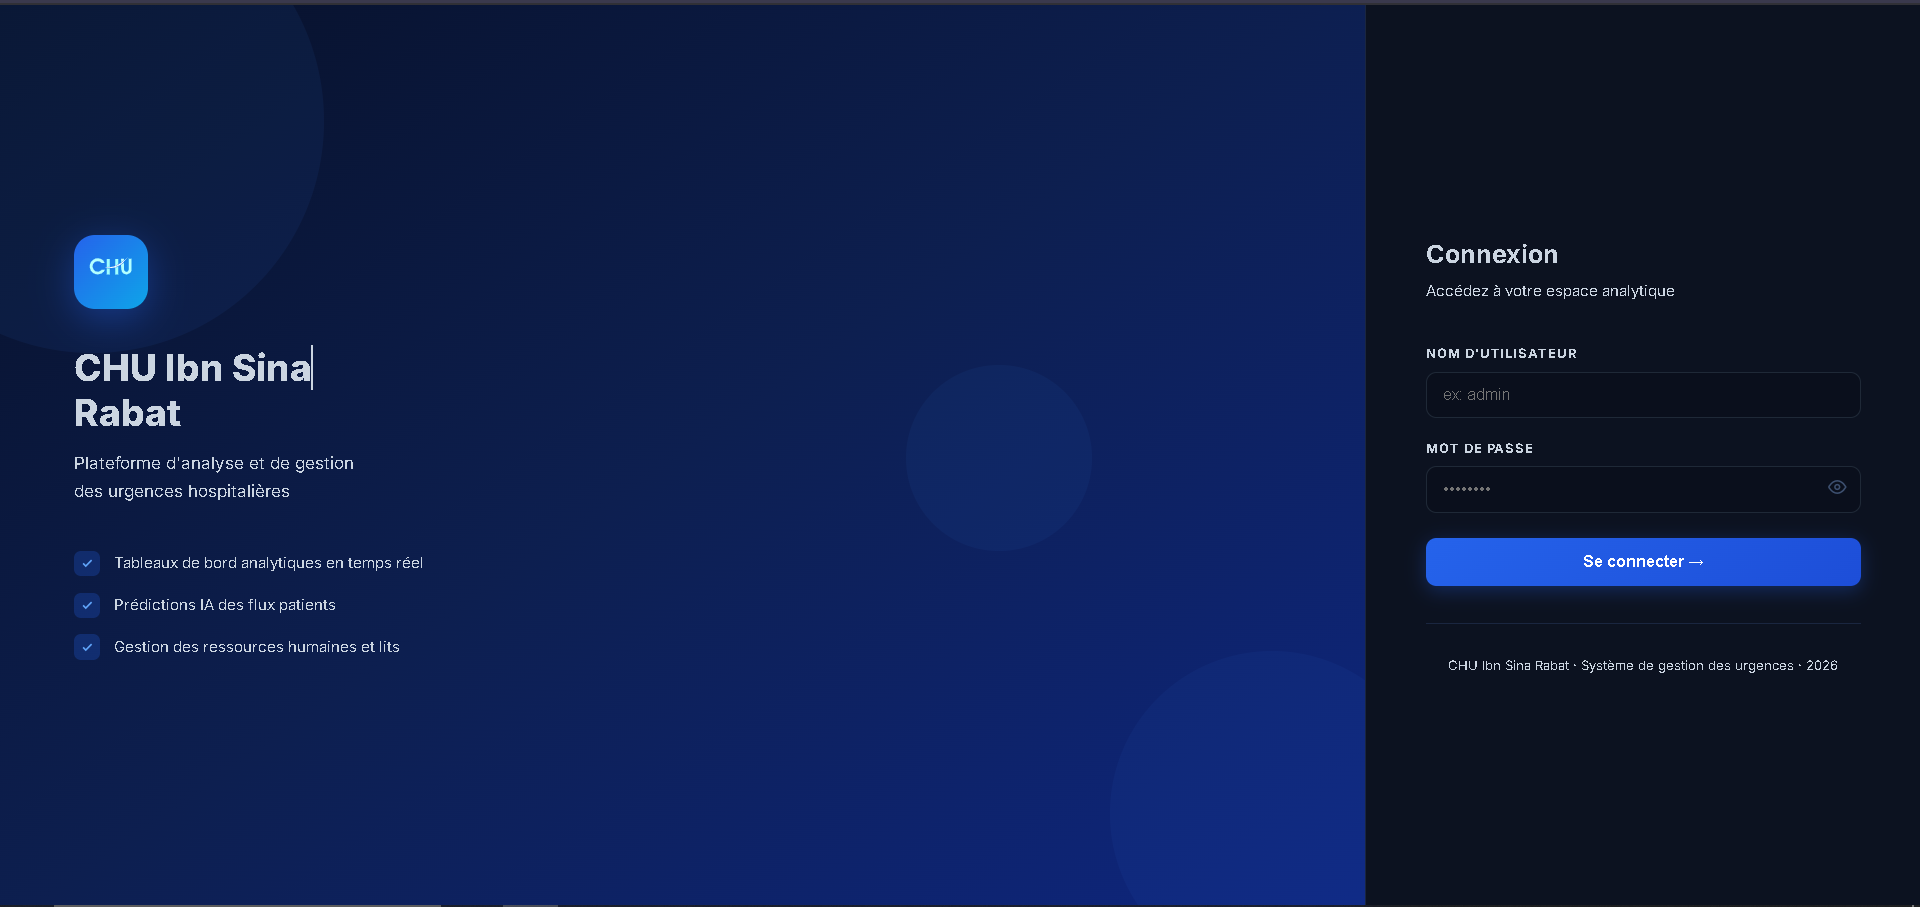
\includegraphics[width=\textwidth]{Login.png}
		\caption{Page de connexion -- Authentification JWT avec indicateur de session}
	\end{figure}
	
	\subsection{Page 2 -- KPIs Globaux}
	
	La page d'accueil présente les indicateurs de performance sous forme de cartes synthétiques
	avec code couleur (vert / orange / rouge selon les seuils). Un filtre par année,
	établissement et orientation permet de personnaliser la vue.
	
	\begin{figure}[H]
		\centering
		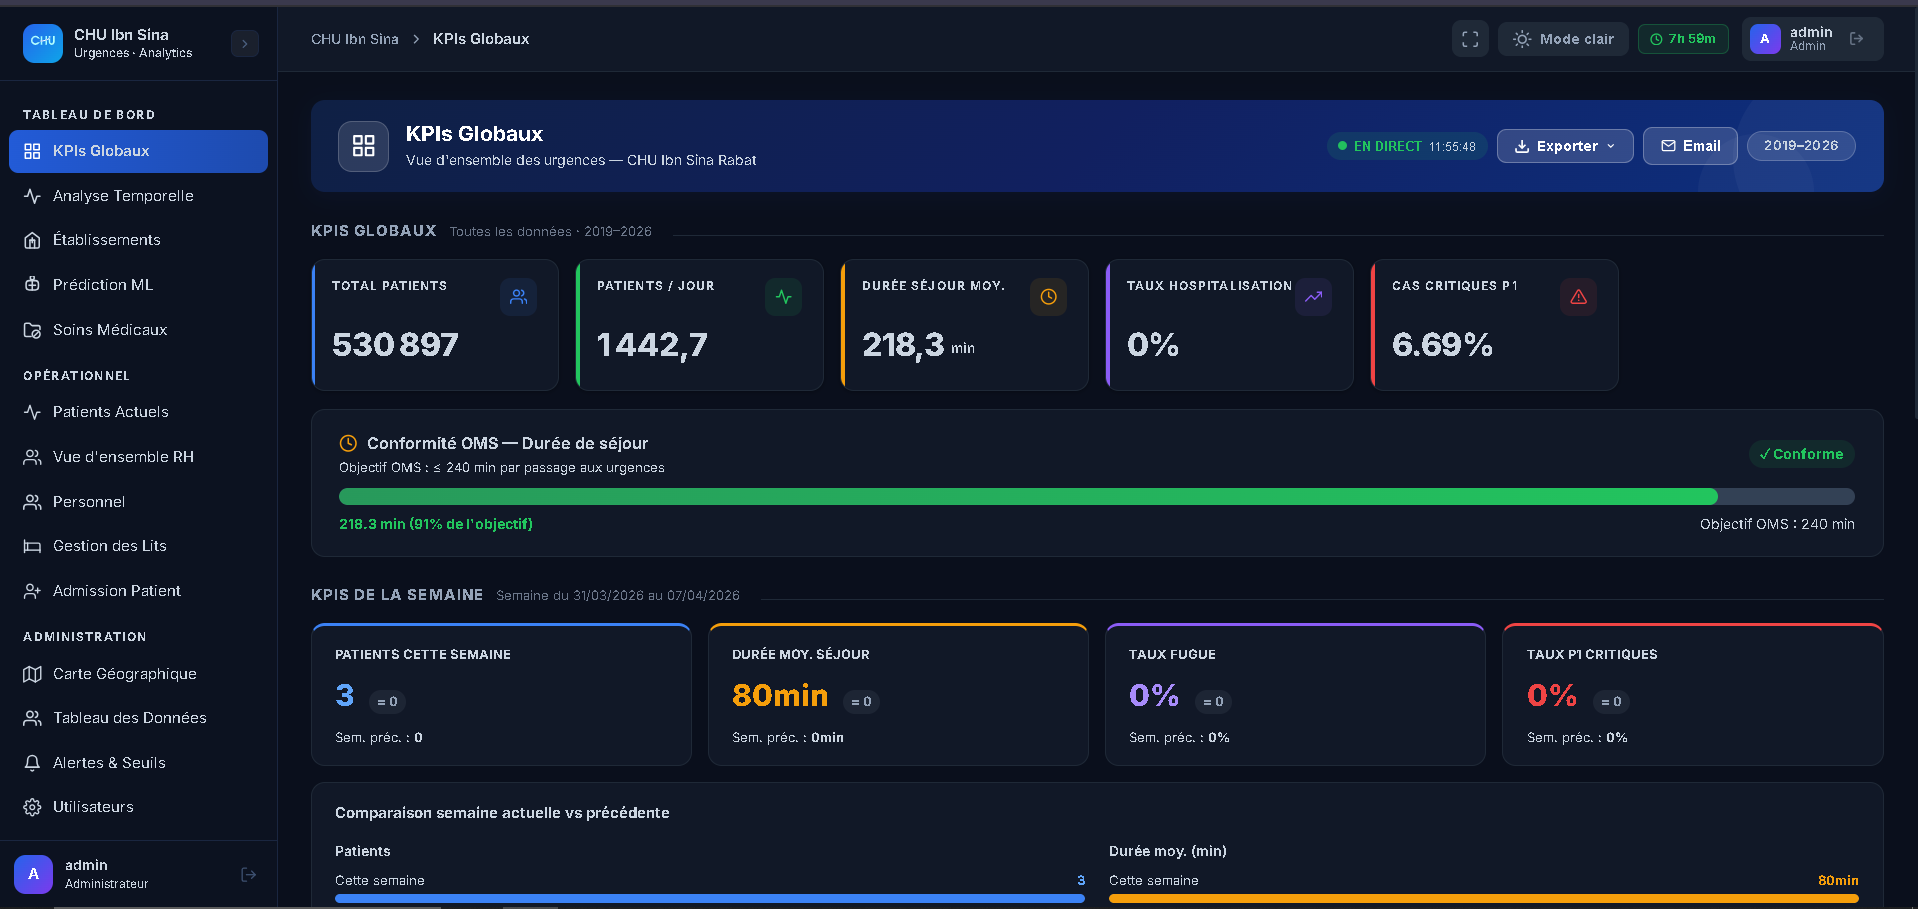
\includegraphics[width=\textwidth]{KPIGlob.png}
		\caption{Page KPIs Globaux -- Vue d'ensemble des indicateurs de performance}
	\end{figure}
	
	\subsection{Page 3 -- Analyse Temporelle}
	
	Cette page offre une analyse multidimensionnelle des flux de patients : distributions
	horaire, hebdomadaire, mensuelle et saisonnière. Une heatmap croisée heure $\times$
	jour de la semaine révèle les pics d'affluence avec une précision à l'heure.
	
	\begin{figure}[H]
		\centering
		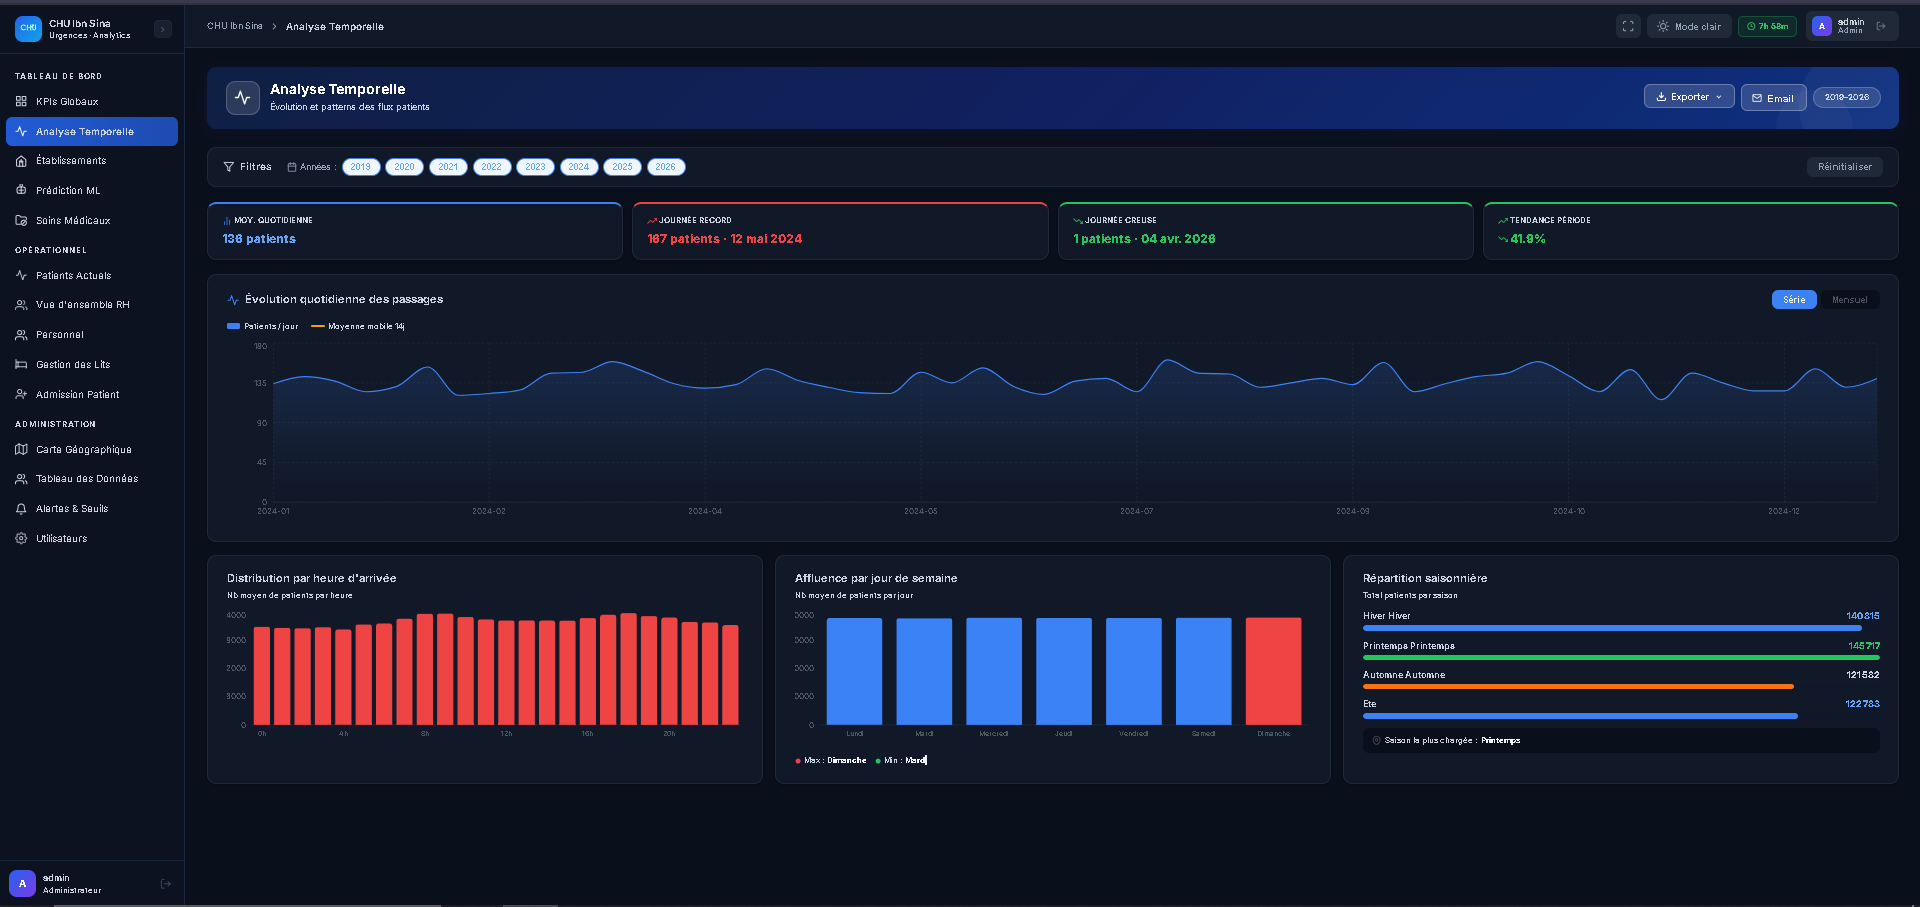
\includegraphics[width=\textwidth]{Analyse temp.png}
		\caption{Page Analyse Temporelle -- Heatmap et distributions multi-dimensionnelles}
	\end{figure}
	
	\subsection{Page 4 -- Prédictions IA}
	
	La page Prédictions IA regroupe six modules analytiques complémentaires accessibles
	via des onglets. Elle constitue le cœur de la valeur ajoutée du dashboard en proposant
	des capacités prévisionnelles basées sur trois algorithmes de Machine Learning distincts.
	
	\subsubsection*{Modèles \& Performance}
	Ce premier onglet présente les métriques d'évaluation des trois modèles entraînés :
	XGBoost (régression des flux), Random Forest (classification de l'orientation) et Prophet
	(séries temporelles). Les indicateurs MAE, RMSE et F1-score sont affichés pour chaque modèle,
	permettant au responsable de juger la fiabilité des prédictions.
	
	\subsubsection*{Prédiction d'orientation}
	Ce module innovant prédit l'orientation probable d'un patient (Hospitalisation, Retour domicile,
	Transfert, Fugue) à partir de son profil clinique. La prédiction est basée sur les statistiques
	conditionnelles calculées sur les 530~914 passages historiques : le système recherche les cas
	similaires selon le niveau de triage, le motif de consultation et le groupe d'âge, puis calcule
	la distribution réelle des orientations pour ce profil. Un indicateur de confiance précise le
	nombre de cas similaires trouvés dans la base.
	
	\begin{figure}[H]
		\centering
		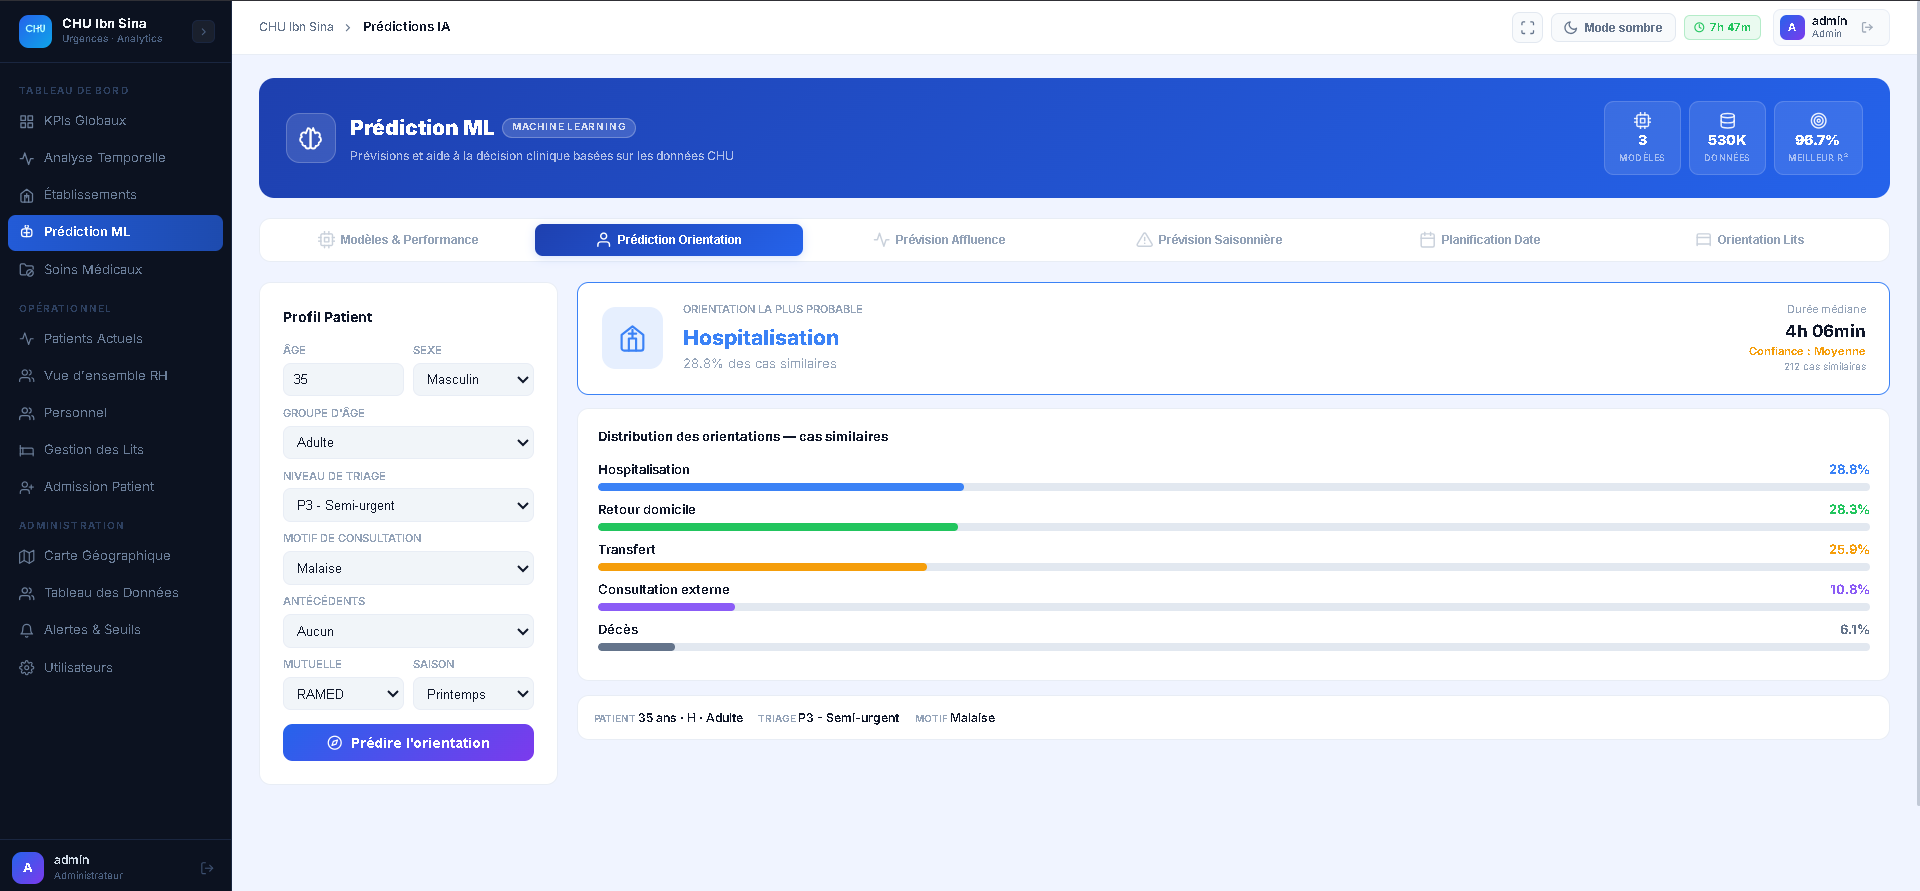
\includegraphics[width=\textwidth]{Prediction Orientation.png}
		\caption{Prédiction d'orientation -- Distribution des orientations basée sur les cas historiques similaires}
	\end{figure}
	
	\subsubsection*{Prévision d'affluence et saisonnière}
	Le module de prévision utilise XGBoost pour anticiper le nombre de patients sur les 30 prochains
	jours, en tenant compte des facteurs saisonniers, des jours fériés et des tendances historiques.
	La prévision saisonnière identifie les pathologies dominantes selon la saison pour préparer
	les stocks médicamenteux et les affectations du personnel.
	
	\begin{figure}[H]
		\centering
		\begin{subfigure}[b]{0.49\textwidth}
			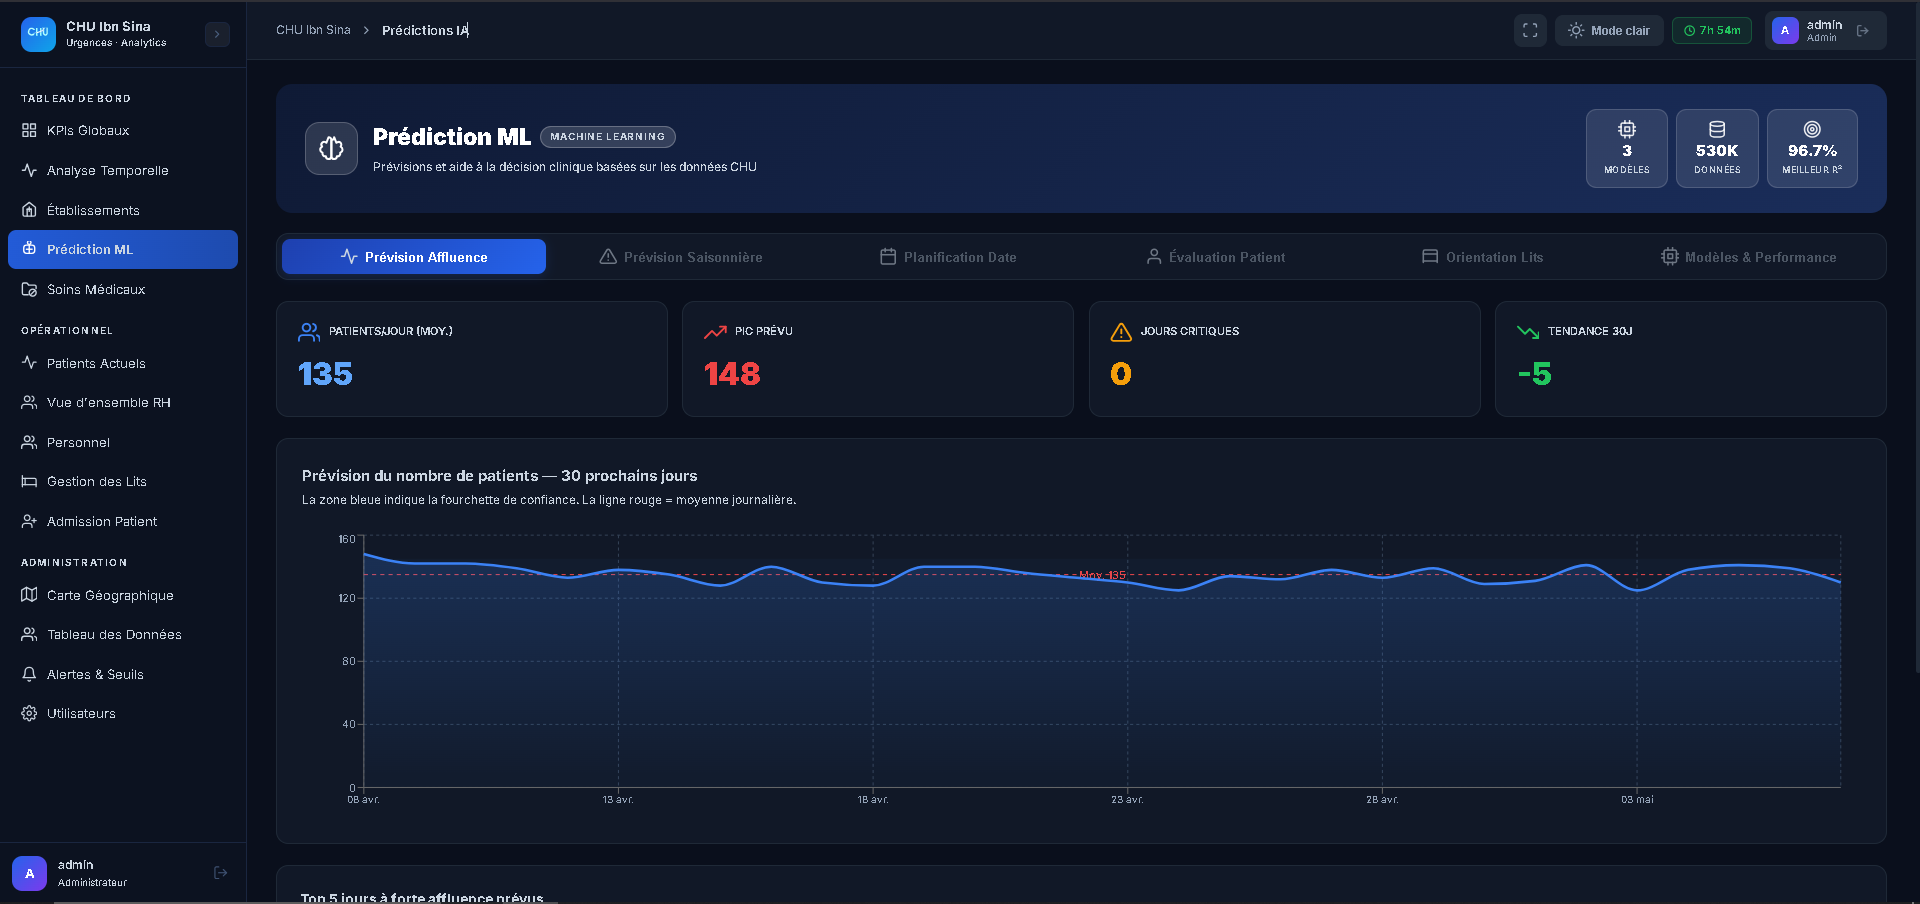
\includegraphics[width=\textwidth]{prevision Affluence.png}
			\caption{Prévision d'affluence 30 jours (XGBoost)}
		\end{subfigure}
		\hfill
		\begin{subfigure}[b]{0.49\textwidth}
			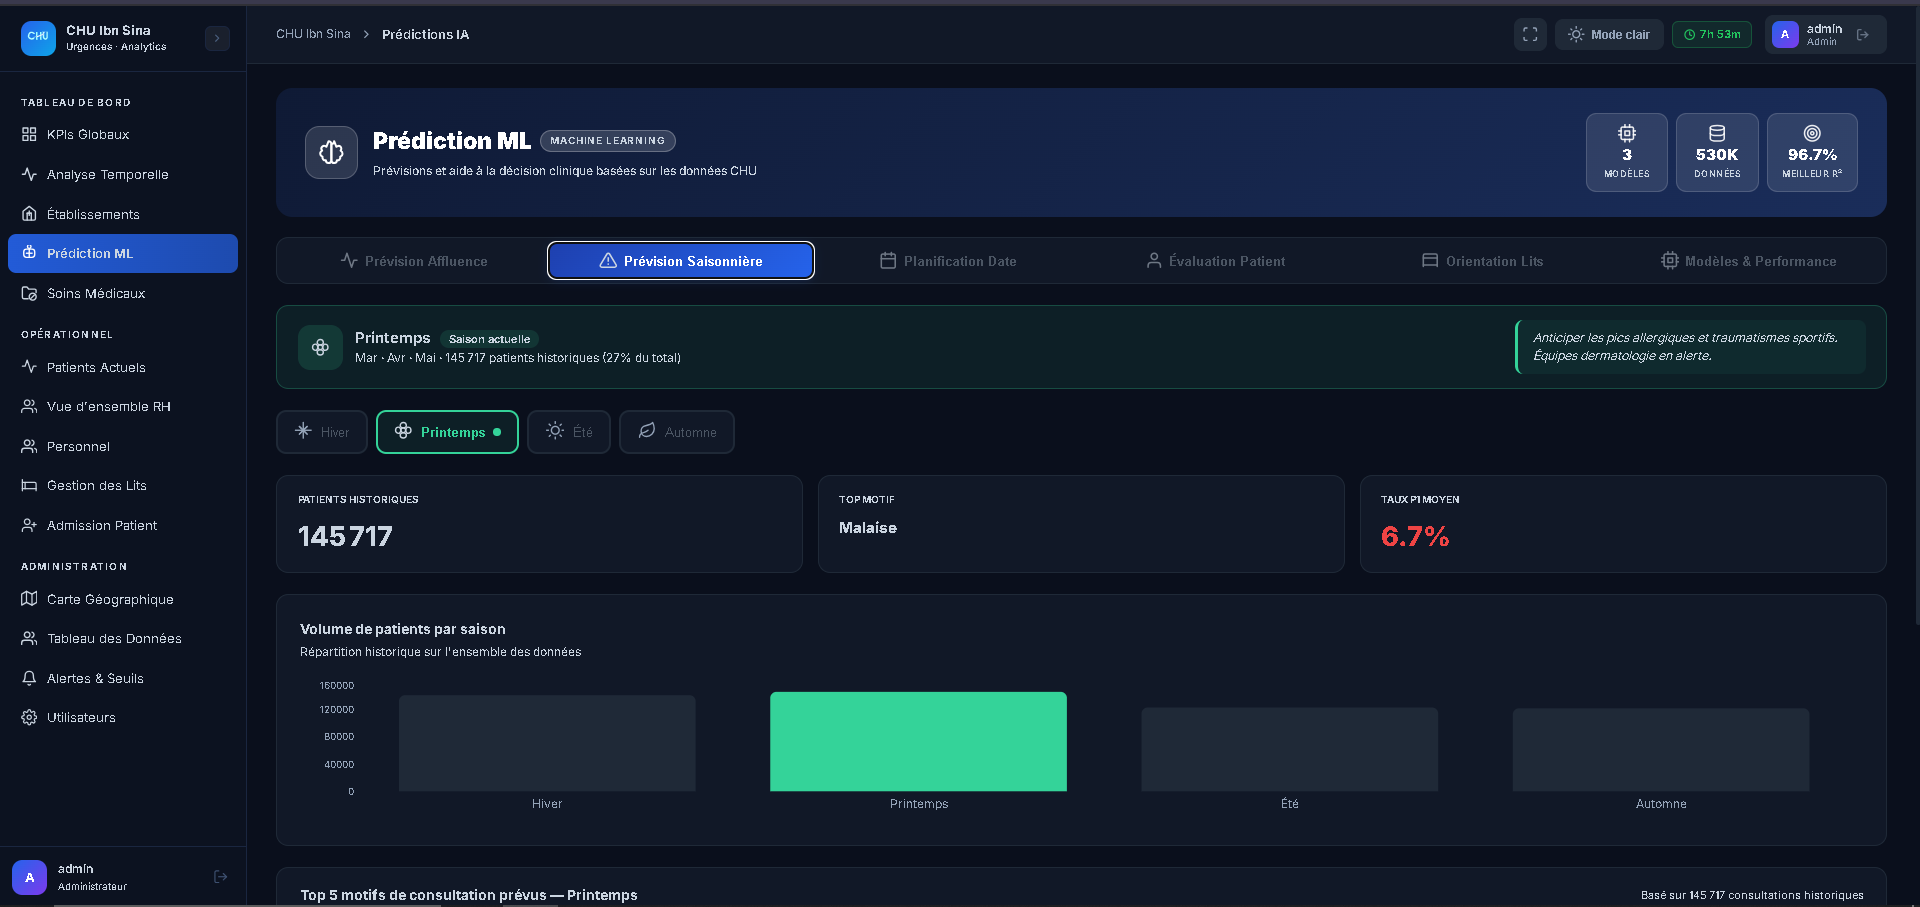
\includegraphics[width=\textwidth]{Prevision Saisonniere.png}
			\caption{Prévision saisonnière des pathologies}
		\end{subfigure}
		\caption{Modules de prévision des flux de patients}
	\end{figure}
	
	\newpage	
	
	\subsubsection*{Planification par date}
	Pour une date future donnée, ce module calcule le nombre de patients attendus, les ressources
	humaines recommandées par spécialité médicale et le nombre de lits nécessaires par service.
	Les recommandations sont basées sur la moyenne historique du même jour de la semaine et du même
	mois, multipliée par un facteur d'ajustement selon la charge prévisionnelle.
	
	\begin{figure}[H]
		\centering
		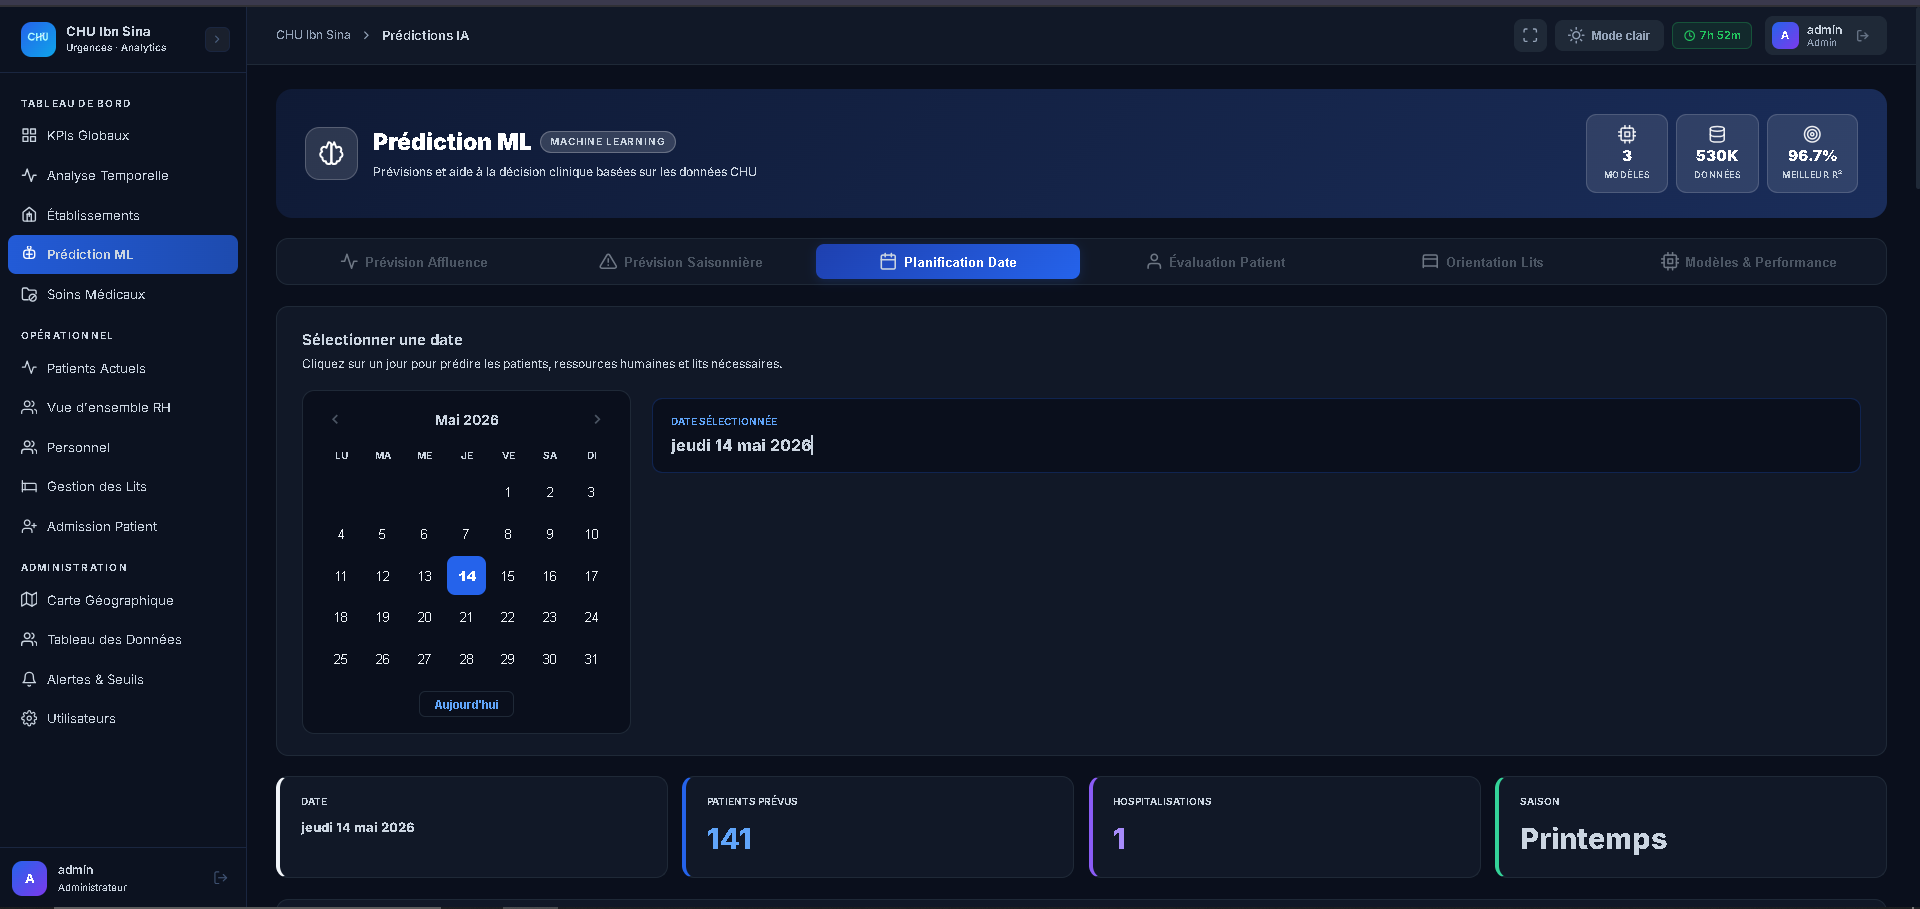
\includegraphics[width=\textwidth]{Planification Date.png}
		\caption{Planification par date -- Recommandations automatiques RH et lits}
	\end{figure}
	\newpage
	\subsection{Page 5 -- Ressources Humaines}
	
	La page Ressources Humaines offre une analyse croisée entre le flux de patients et les
	ressources disponibles. Elle permet aux responsables d'identifier en temps réel les
	déséquilibres entre la demande de soins et l'offre en personnel médical. Les graphiques
	de corrélation flux/médecins disponibles mettent en évidence les périodes de sous-effectif,
	tandis que les indicateurs de saturation par service alertent sur les situations critiques
	avant qu'elles ne se produisent.
	
	Les indicateurs calculés comprennent le ratio médecins par patient, le taux d'occupation
	par spécialité, et la comparaison entre l'effectif actuel et l'effectif recommandé par
	les modèles de planification.
	
	\begin{figure}[H]
		\centering
		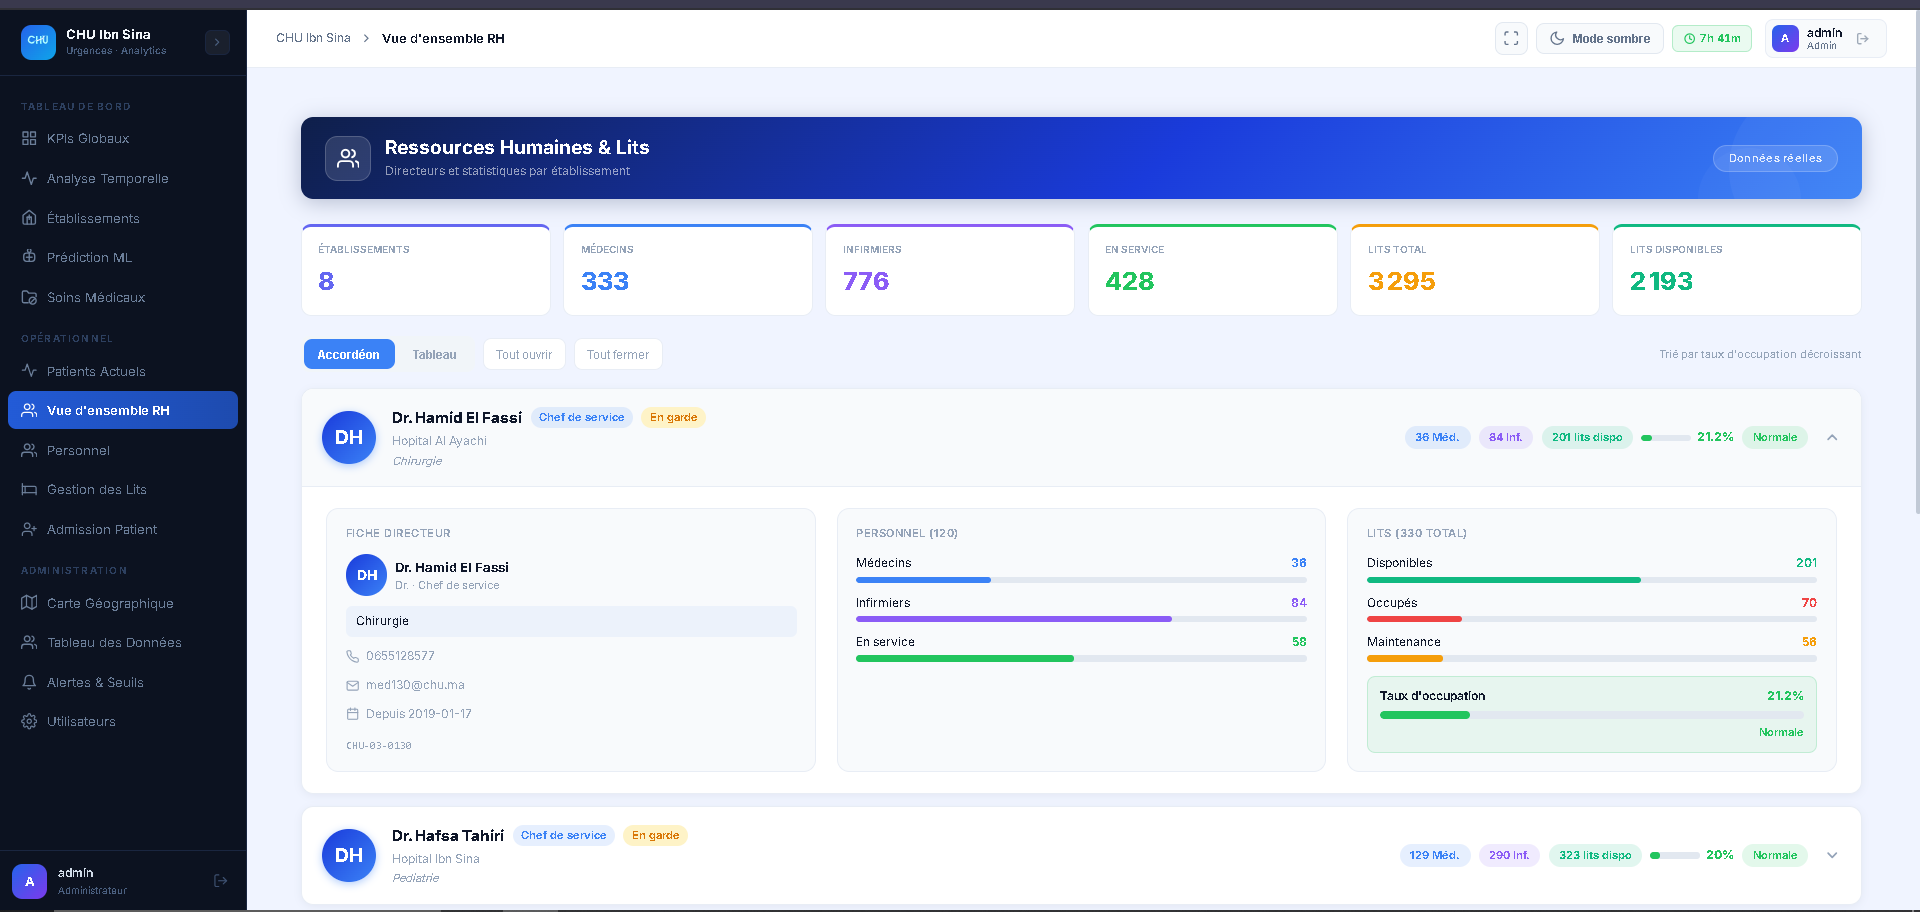
\includegraphics[width=\textwidth]{vue RH.png}
		\caption{Vue Ressources Humaines -- Corrélation flux patients / personnel disponible par service}
	\end{figure}
	\newpage
	\subsection{Page 6 -- Soins Médicaux}
	
	Cette page analyse l'ensemble des 737~512 actes médicaux enregistrés dans la base de données.
	Elle présente la répartition des types de soins, les coûts moyens par établissement et par
	service, ainsi que la distribution des modes de financement (AMO, RAMED, Payant, Assurance,
	Exonération réglementée). Ces informations sont essentielles pour la direction financière afin
	d'optimiser la politique tarifaire et de piloter les conventions avec les organismes de
	remboursement.
	
	Les graphiques permettent d'identifier les actes les plus coûteux, les services les plus
	consommateurs de ressources et les tendances d'évolution des coûts dans le temps.
	
	\begin{figure}[H]
		\centering
		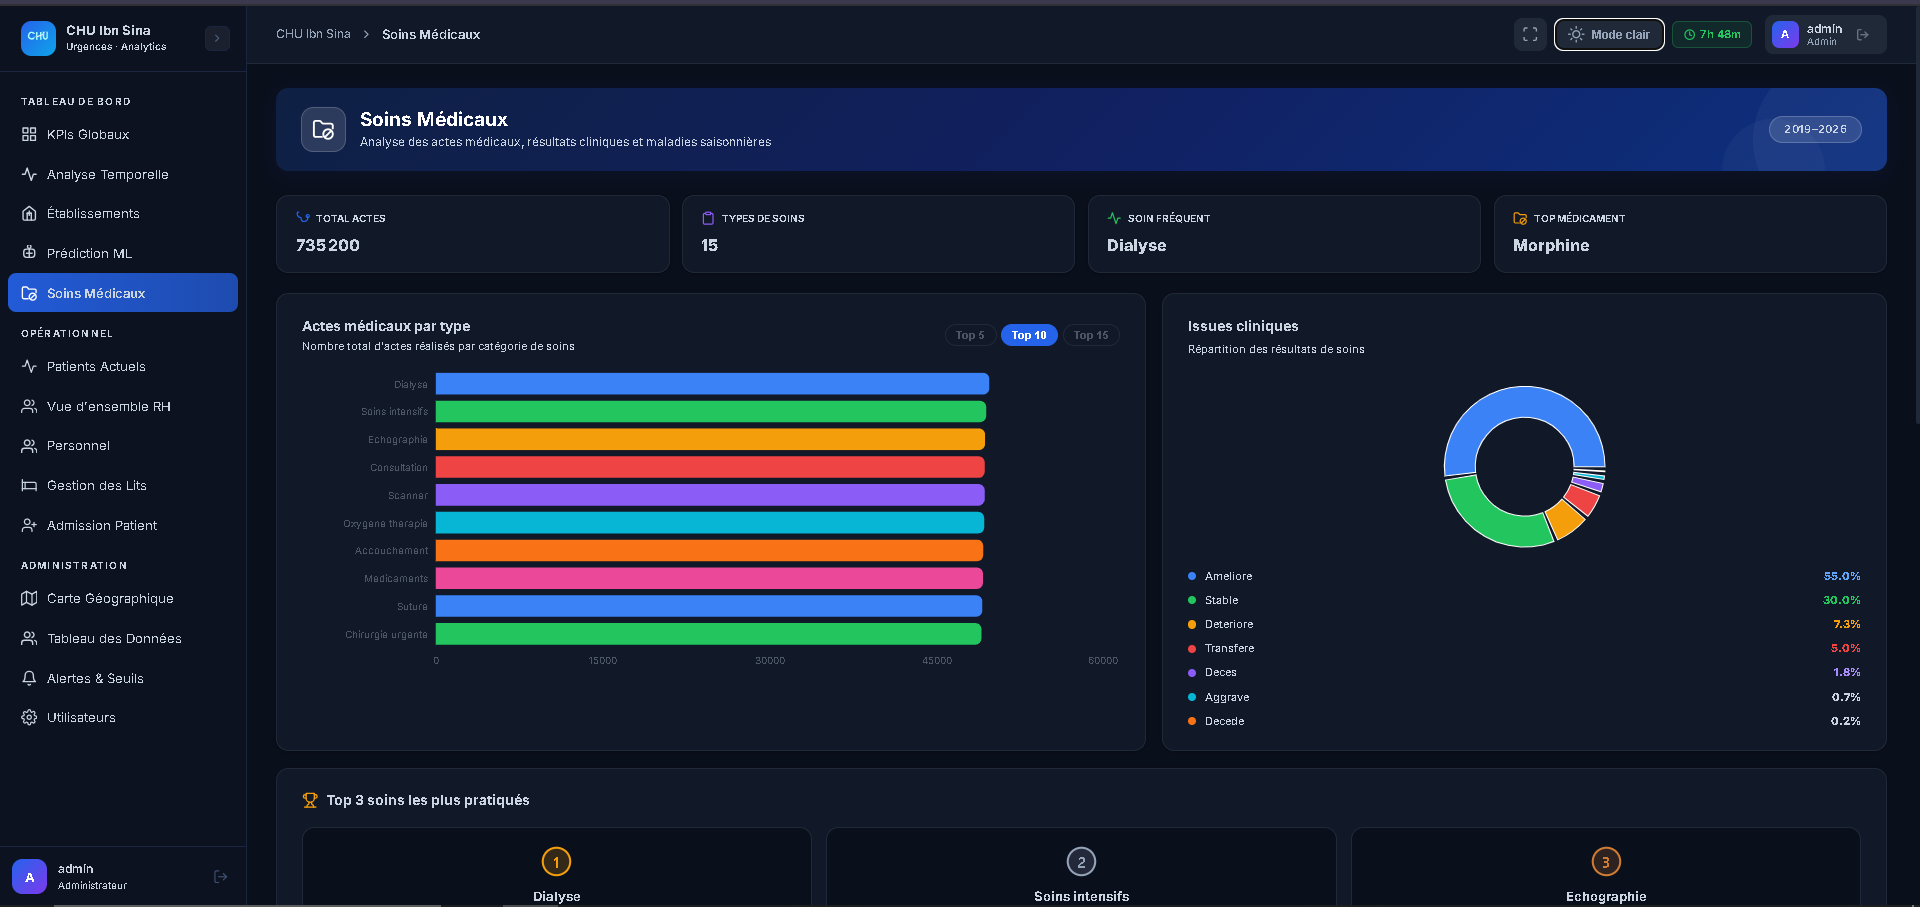
\includegraphics[width=\textwidth]{Soins medicaux.png}
		\caption{Page Soins Médicaux -- Analyse des coûts et répartition des financements}
	\end{figure}
	
	\subsection{Page 7 -- Patients Actuels}
	
	La page Patients Actuels constitue le module de suivi opérationnel en temps réel. Elle
	affiche l'ensemble des patients admis dans les \textbf{24 dernières heures glissantes}
	et se rafraîchit automatiquement toutes les 30 secondes. Chaque patient est affiché avec
	son heure d'arrivée, son niveau de triage (code couleur P1 à P4), son motif de consultation
	et son statut clinique actuel.
	
	Les fonctionnalités principales de cette page sont :
	\begin{itemize}
		\item \textbf{Gestion des statuts} : progression En triage $\to$ En attente $\to$ En traitement $\to$ Sorti,
		modifiable en un clic ;
		\item \textbf{Attribution de lit} : sélection du lit disponible depuis un menu déroulant groupé
		par hôpital, avec mise à jour immédiate en base de données ;
		\item \textbf{Filtres combinables} : par statut, niveau de triage (P1 à P4) et recherche textuelle
		sur le nom, CIN ou motif ;
		\item \textbf{Double vue} : mode accordéon (regroupement par établissement) et mode tableau global ;
		\item \textbf{KPIs temps réel} : admissions du jour, patients actifs, taux d'occupation des lits,
		taux de criticité P1.
	\end{itemize}
	
	\begin{figure}[H]
		\centering
		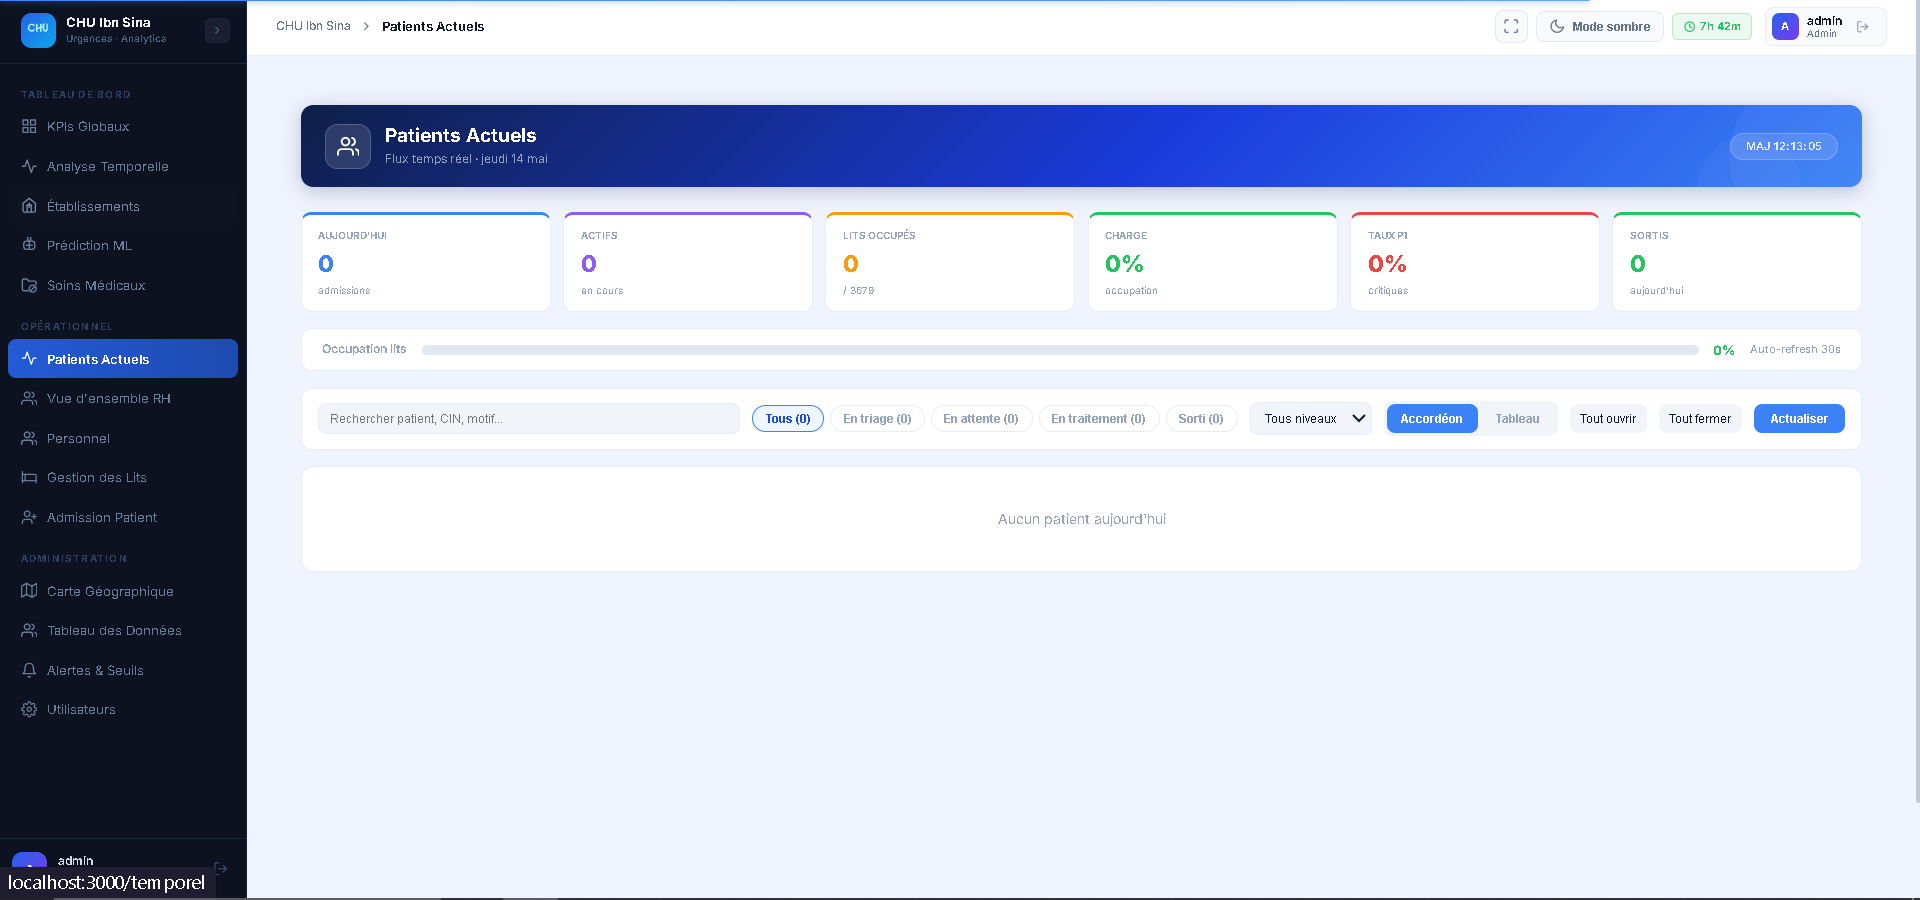
\includegraphics[width=\textwidth]{Patient Actuels.png}
		\caption{Page Patients Actuels -- Suivi temps réel avec KPIs et attribution de lits}
	\end{figure}
	
	\subsection{Page 8 -- Admission Patient}
	
	Le formulaire d'admission permet de saisir un nouveau patient directement depuis l'interface
	web, sans nécessiter d'accès au système d'information hospitalier sous-jacent. Il comprend
	l'ensemble des champs nécessaires à la constitution du dossier urgences : données d'identité,
	groupe sanguin, antécédents, niveau de triage, motif de consultation, orientation prévisionnelle
	et informations financières.
	
	Plusieurs mécanismes automatiques facilitent la saisie :
	\begin{itemize}
		\item La \textbf{date et l'heure d'arrivée} sont pré-renseignées à l'heure locale du serveur ;
		\item Le \textbf{calcul automatique des tarifs} s'adapte à la mutuelle sélectionnée ;
		\item La liste des \textbf{établissements} est chargée dynamiquement depuis la base de données ;
		\item Une \textbf{protection} empêche la saisie de dates futures ou antérieures de plus de 24\,h.
	\end{itemize}
	
	\begin{figure}[H]
		\centering
		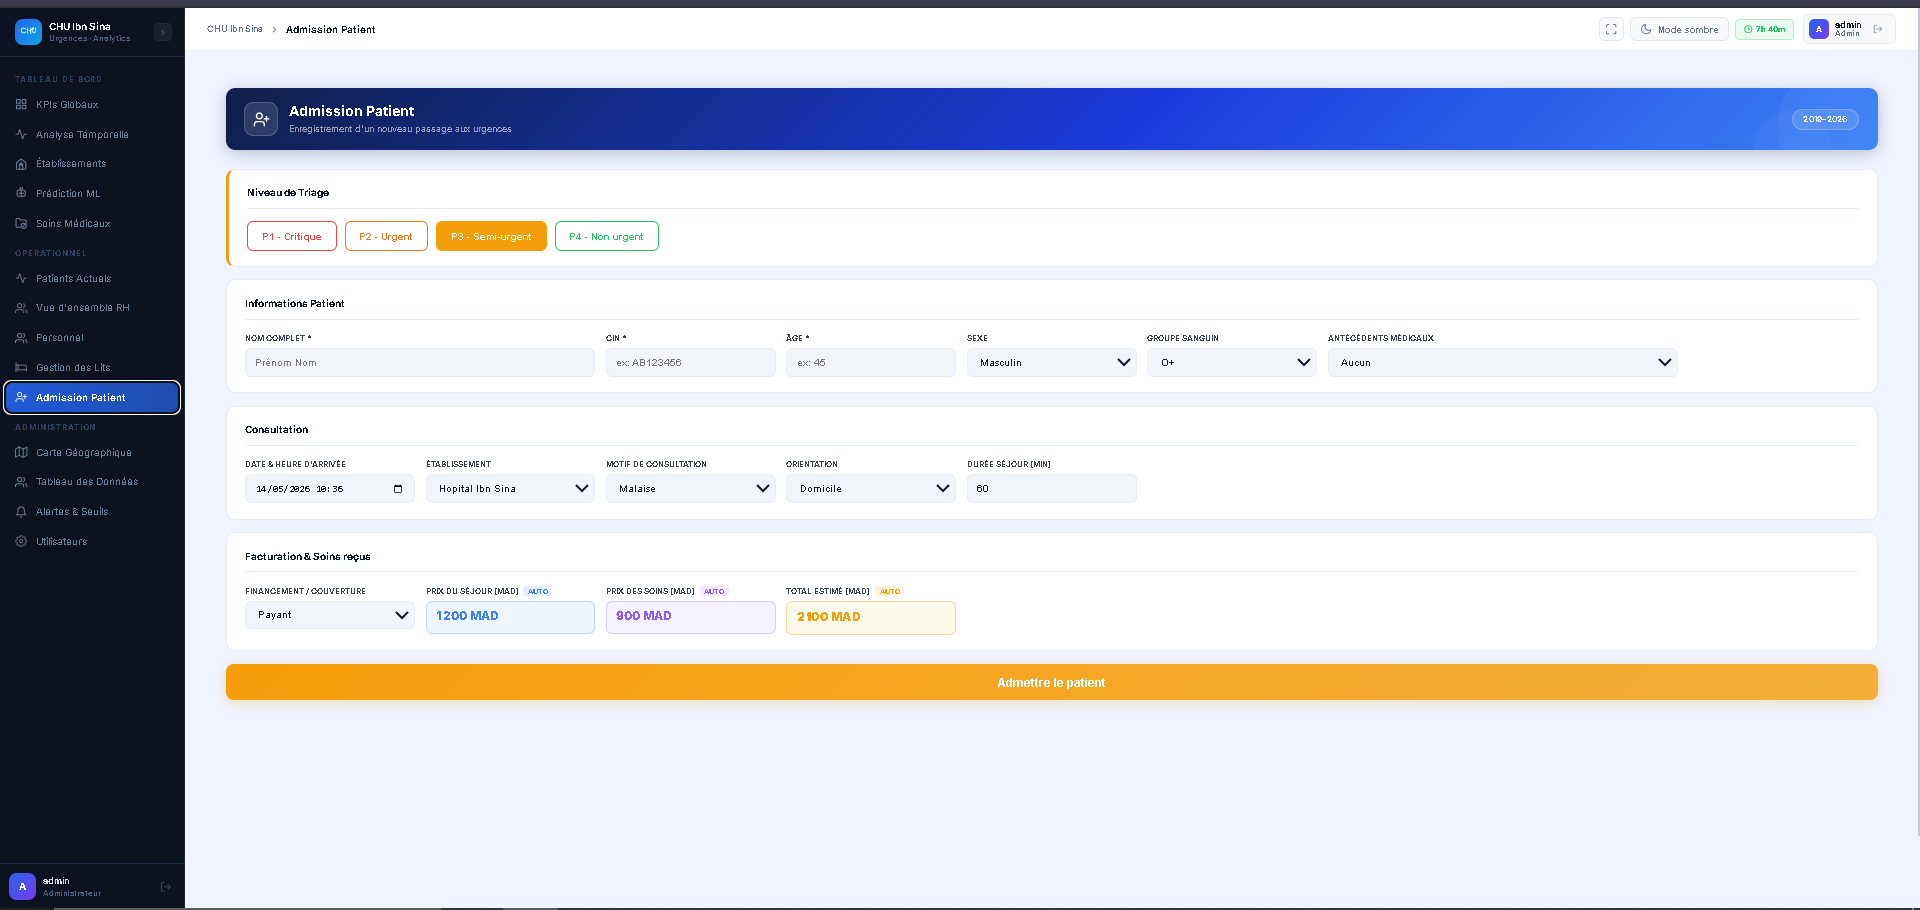
\includegraphics[width=\textwidth]{Admission .png}
		\caption{Formulaire d'admission -- Saisie complète d'un nouveau patient aux urgences}
	\end{figure}
	
	\subsection{Page 9 -- Gestion des Lits}
	
	La page Gestion des Lits offre une vue exhaustive des 3~295 lits répartis dans les 8 hôpitaux
	du réseau CHU Ibn Sina. Chaque lit est caractérisé par son numéro (selon la convention de
	nommage standardisée : UR pour Urgences, RE pour Réanimation, CH pour Chirurgie, etc.),
	son service, son type (Standard, Soins intensifs, Réanimation, Pédiatrique) et son statut
	(Disponible, Occupé, En maintenance).
	
	Le tableau de bord de cette page affiche en temps réel le taux d'occupation global et par
	service, permettant aux équipes logistiques d'anticiper les besoins en lits et d'optimiser
	les rotations. La modification du statut d'un lit s'effectue directement depuis l'interface.
	
	\begin{figure}[H]
		\centering
		\begin{subfigure}[b]{0.49\textwidth}
			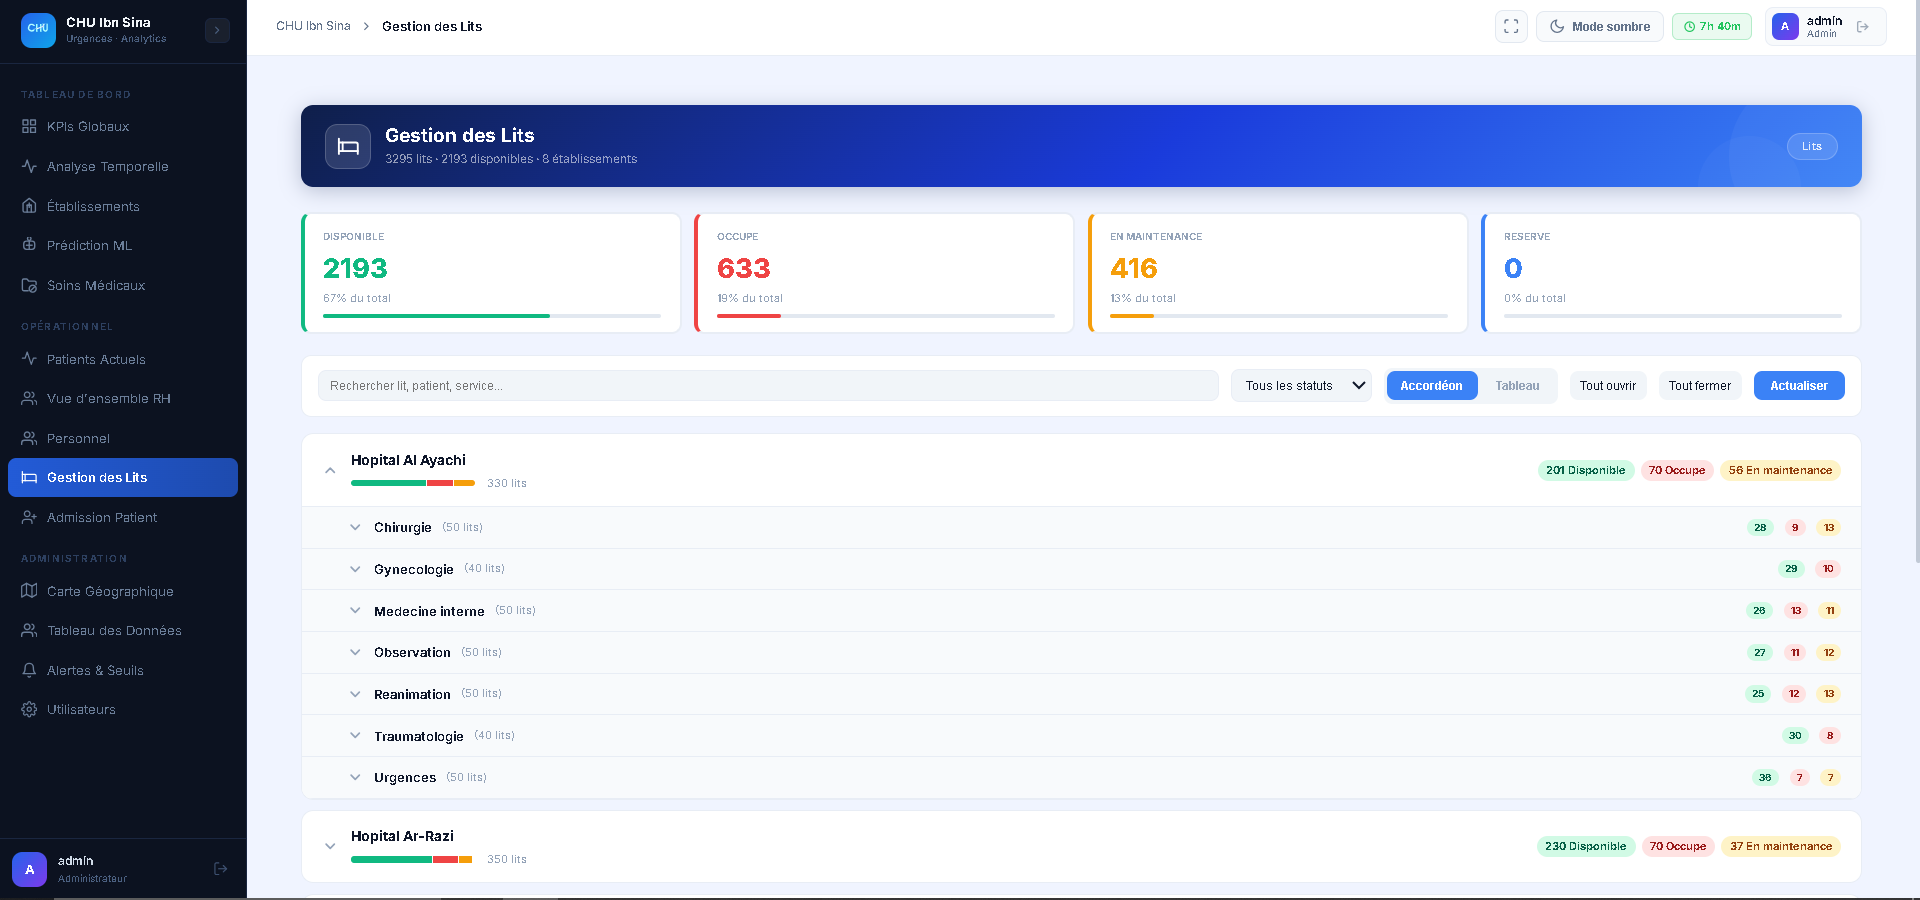
\includegraphics[width=\textwidth]{gestion des lits.png}
			\caption{Inventaire des lits par service}
		\end{subfigure}
		\hfill
		\begin{subfigure}[b]{0.49\textwidth}
			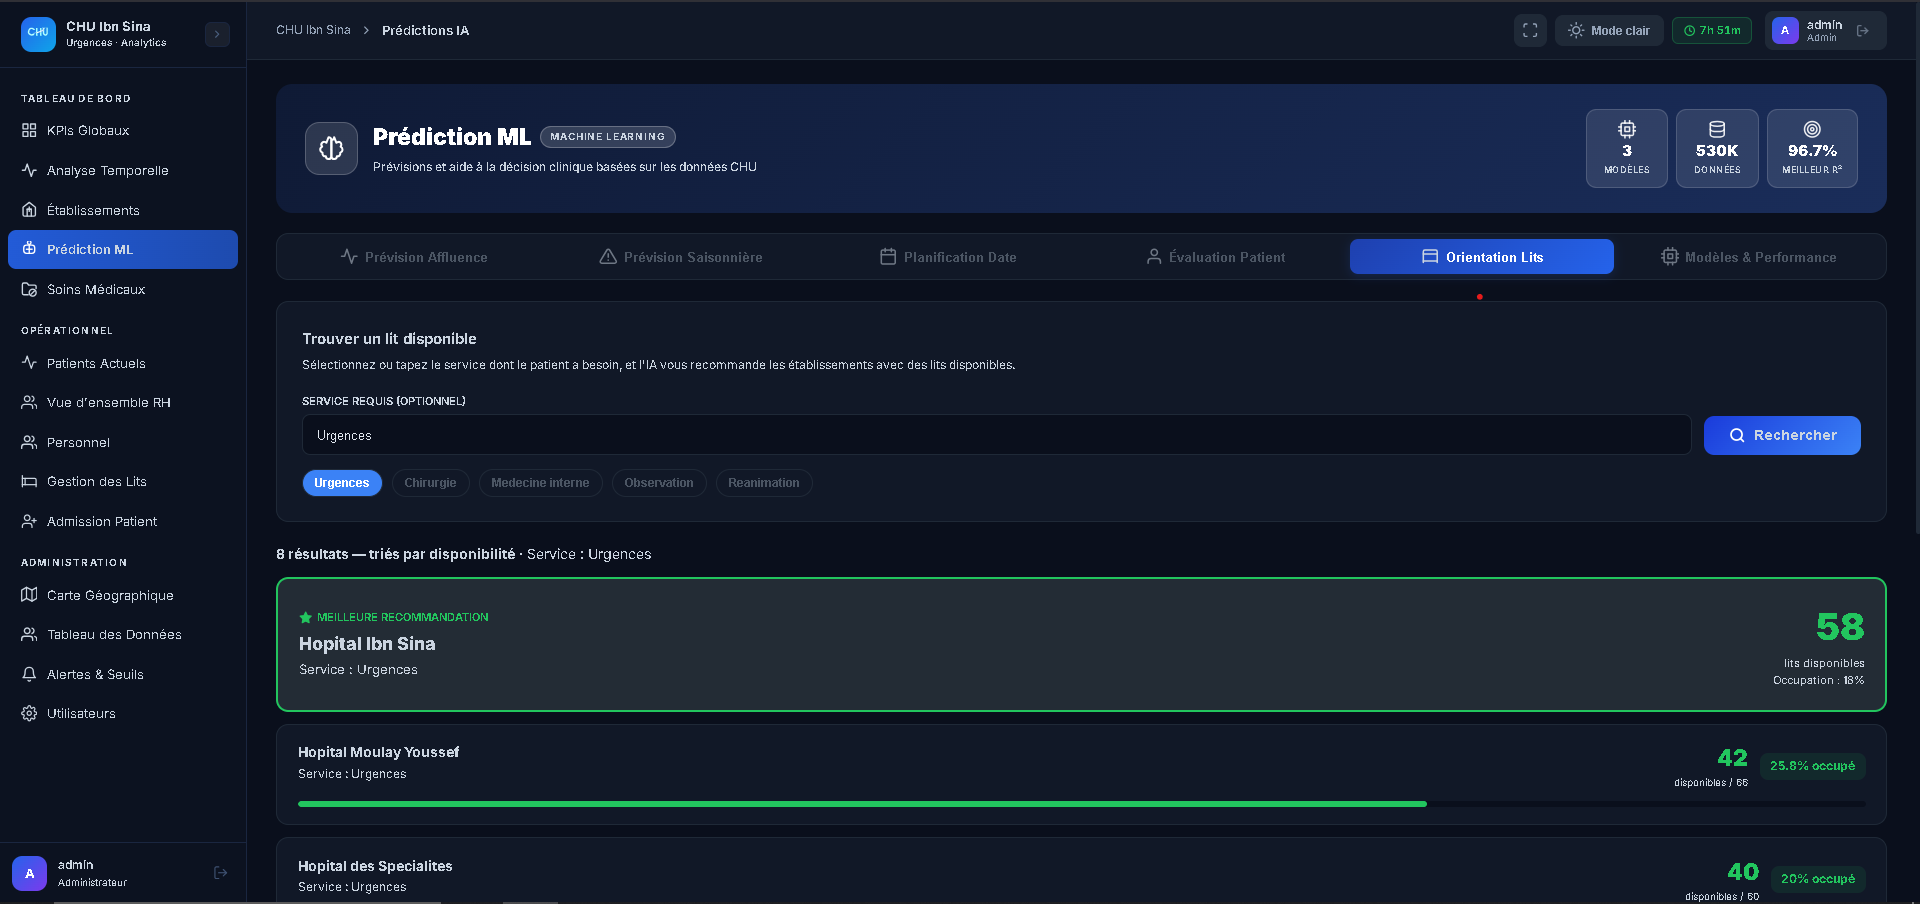
\includegraphics[width=\textwidth]{Orientation Lits.png}
			\caption{Recommandation d'orientation}
		\end{subfigure}
		\caption{Page Gestion des Lits -- Inventaire et taux d'occupation en temps réel}
	\end{figure}
	
	\subsection{Page 10 -- Gestion du Personnel}
	
	La page Gestion du Personnel présente l'annuaire complet des 1~086 membres du personnel
	médical et soignant. Chaque fiche contient la spécialité médicale, le statut de service
	(En service / En garde / En congé), le matricule et l'établissement d'affectation.
	Des filtres par spécialité et par établissement permettent une navigation rapide dans
	l'annuaire. Un graphique de répartition visualise la distribution des spécialités au sein
	de chaque hôpital, facilitant le repérage des services sous-dotés.
	
	\begin{figure}[H]
		\centering
		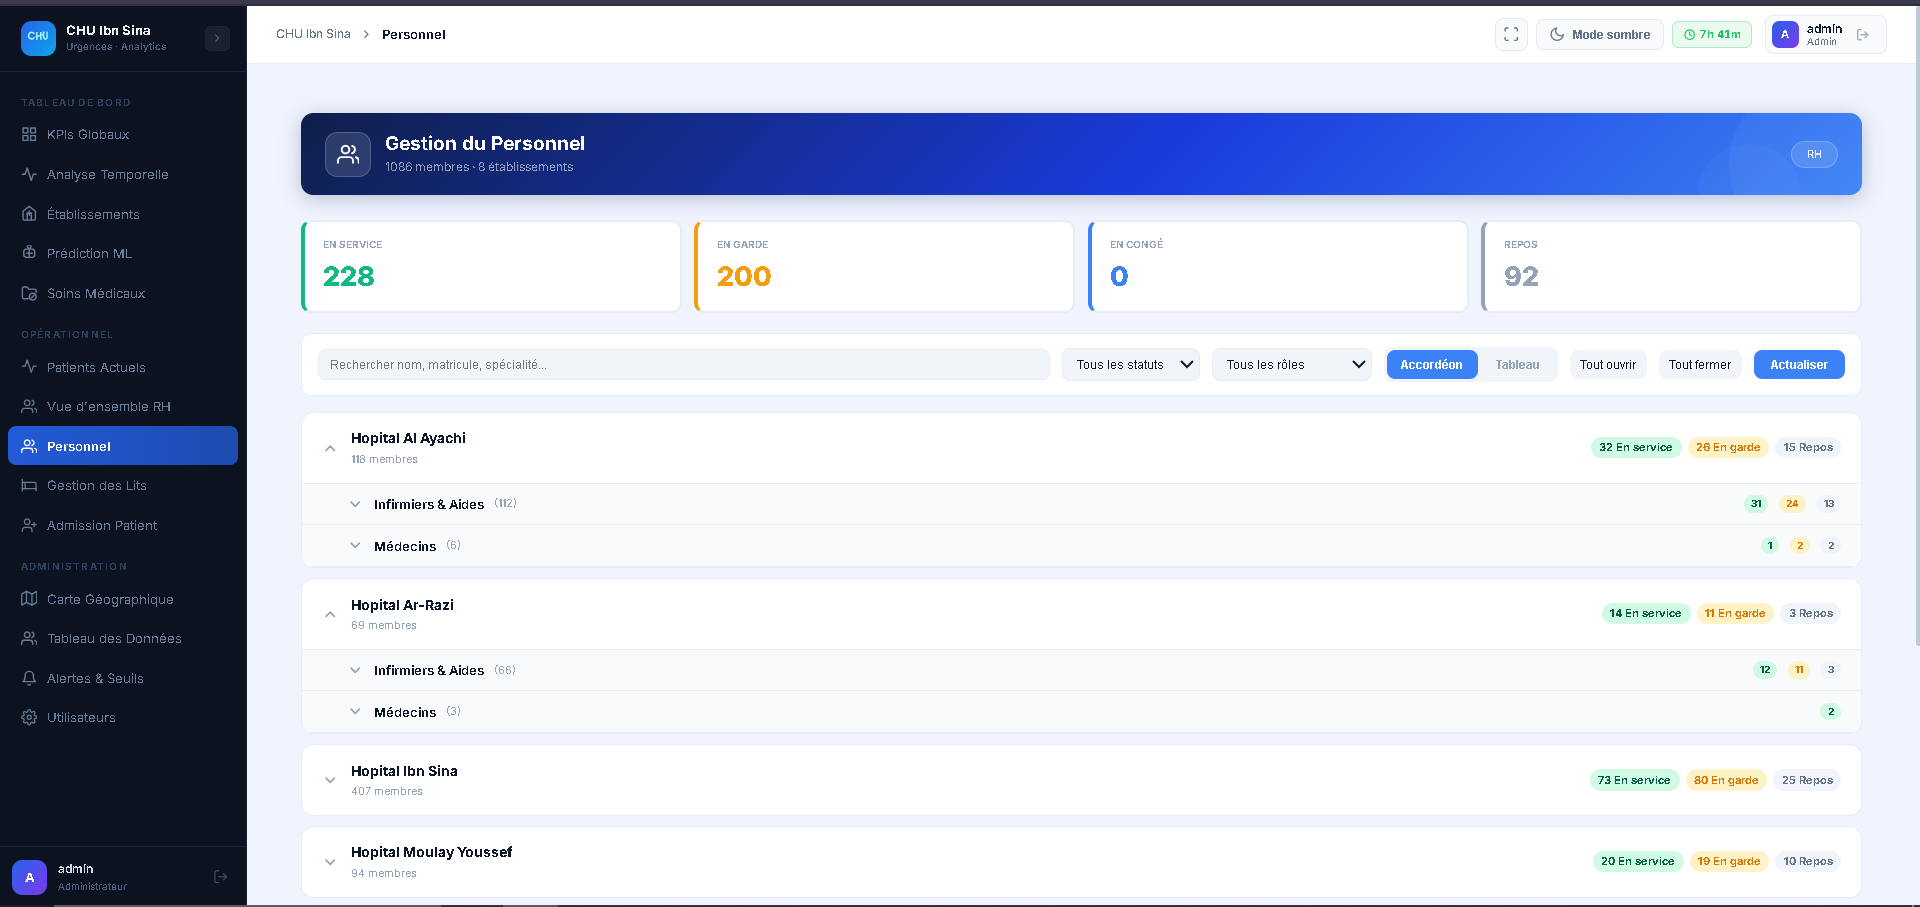
\includegraphics[width=\textwidth]{personnel.png}
		\caption{Page Gestion du Personnel -- Annuaire et répartition par spécialité}
	\end{figure}
	
	\subsection{Pages 11 à 15}
	
	\begin{figure}[H]
		\centering
		\begin{subfigure}[b]{0.48\textwidth}
			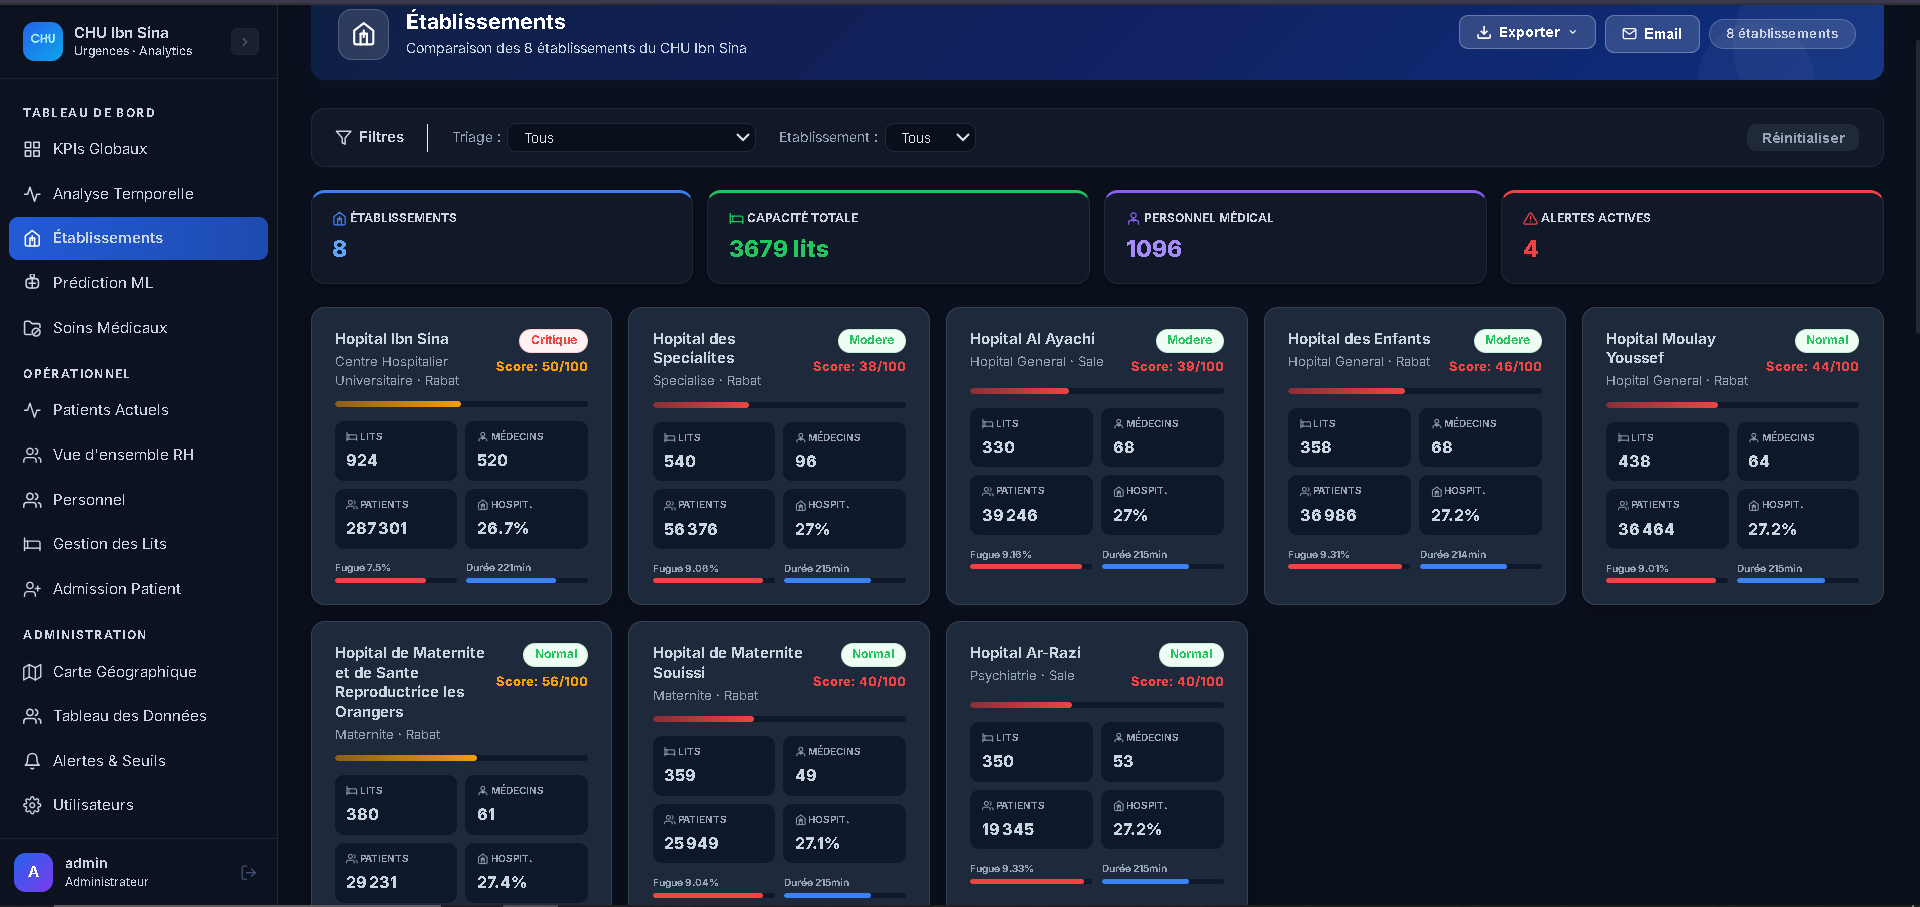
\includegraphics[width=\textwidth]{Etablissement.png}
			\caption{Établissements (P.11)}
		\end{subfigure}
		\hfill
		\begin{subfigure}[b]{0.48\textwidth}
			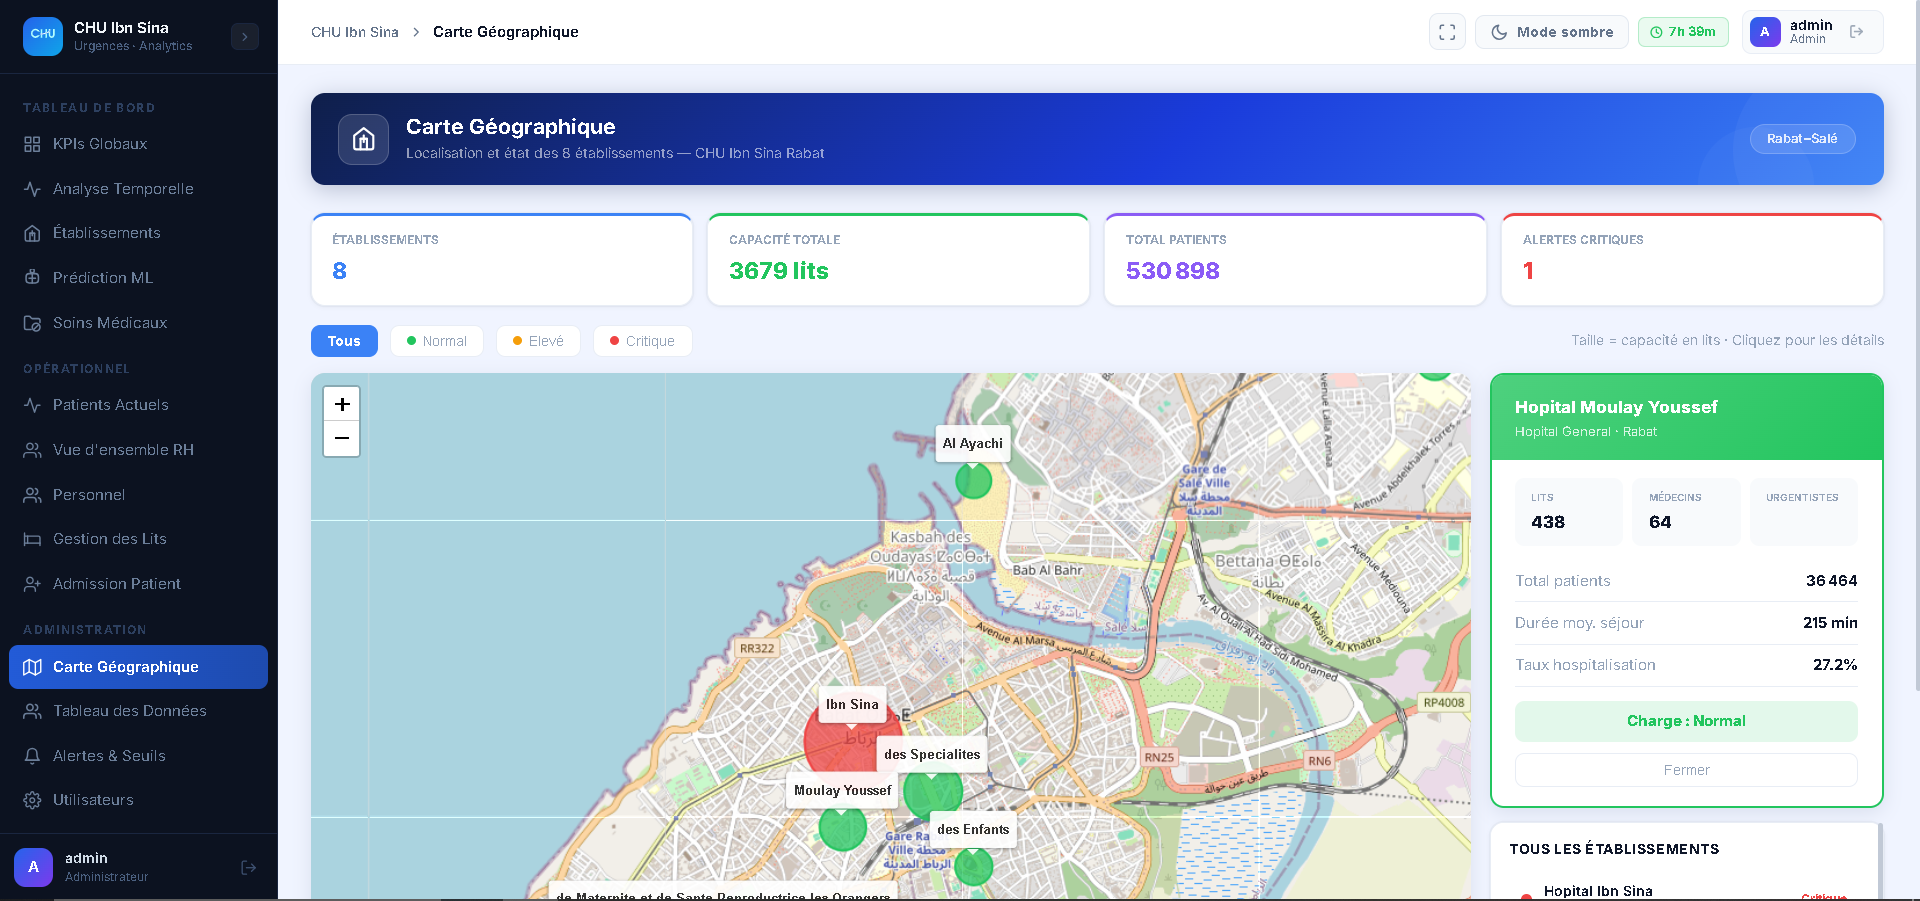
\includegraphics[width=\textwidth]{Carte Geo.png}
			\caption{Carte Géographique (P.12)}
		\end{subfigure}
		
		\vspace{0.4cm}
		
		\begin{subfigure}[b]{0.48\textwidth}
			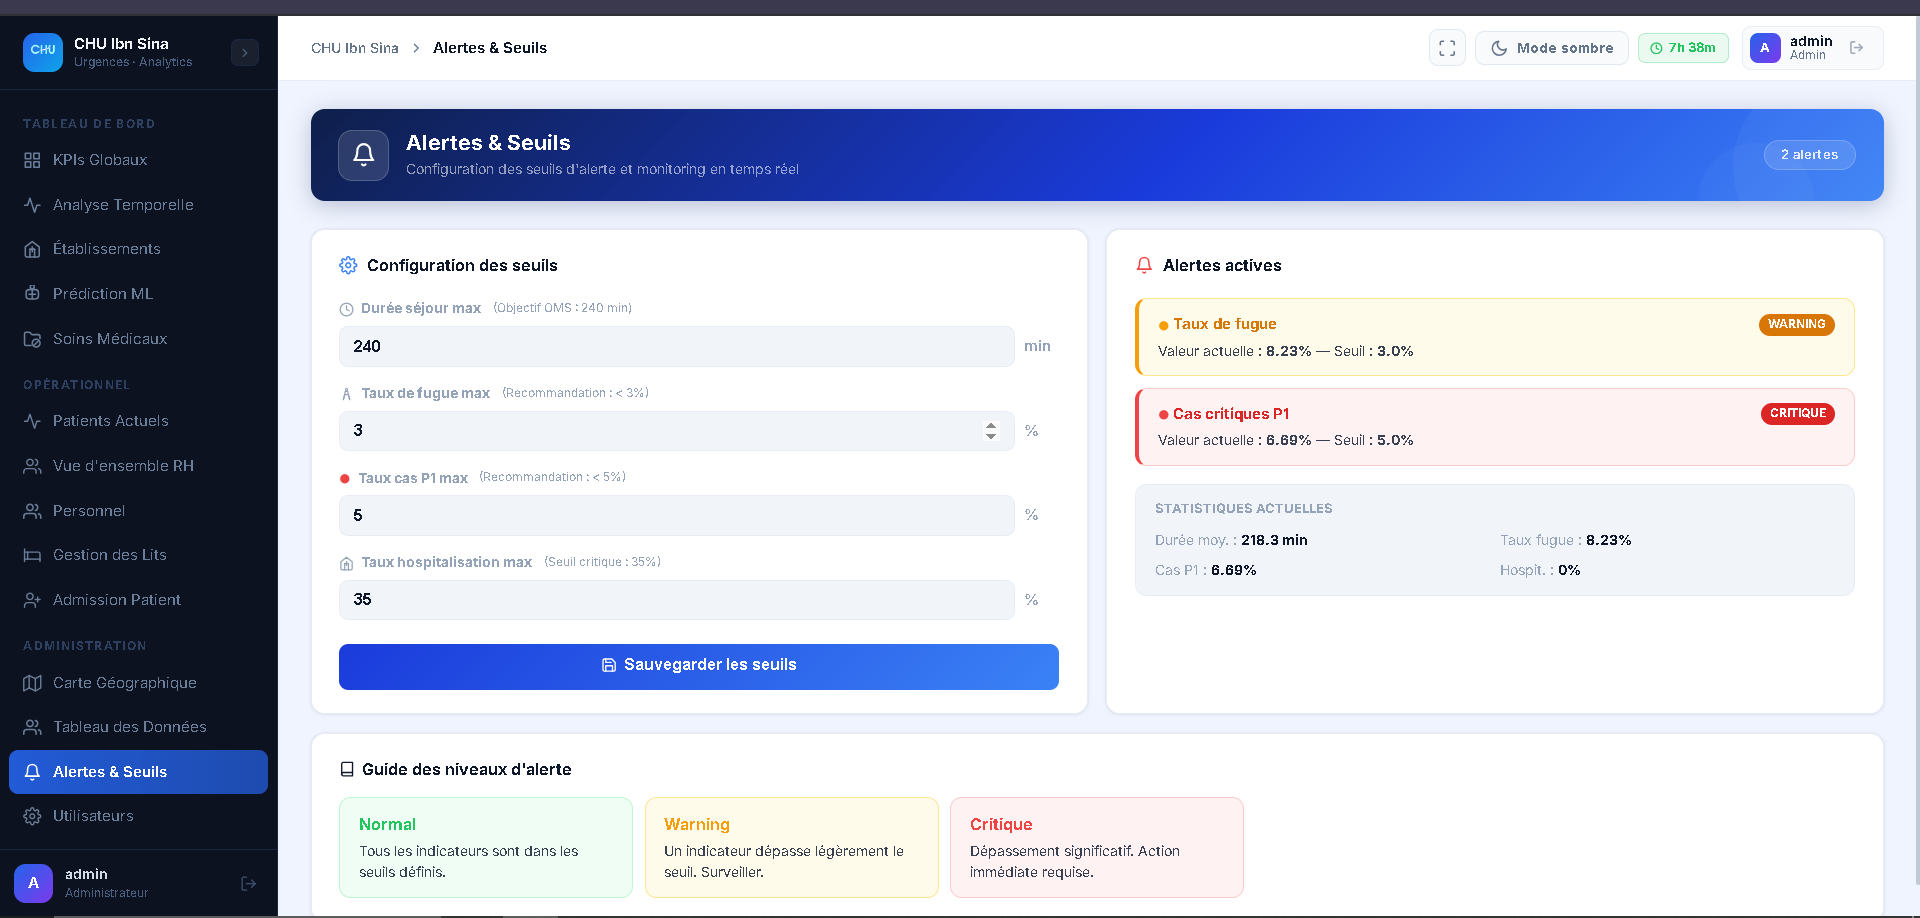
\includegraphics[width=\textwidth]{Alertes et Seuils.png}
			\caption{Alertes \& Seuils (P.13)}
		\end{subfigure}
		\hfill
		\begin{subfigure}[b]{0.48\textwidth}
			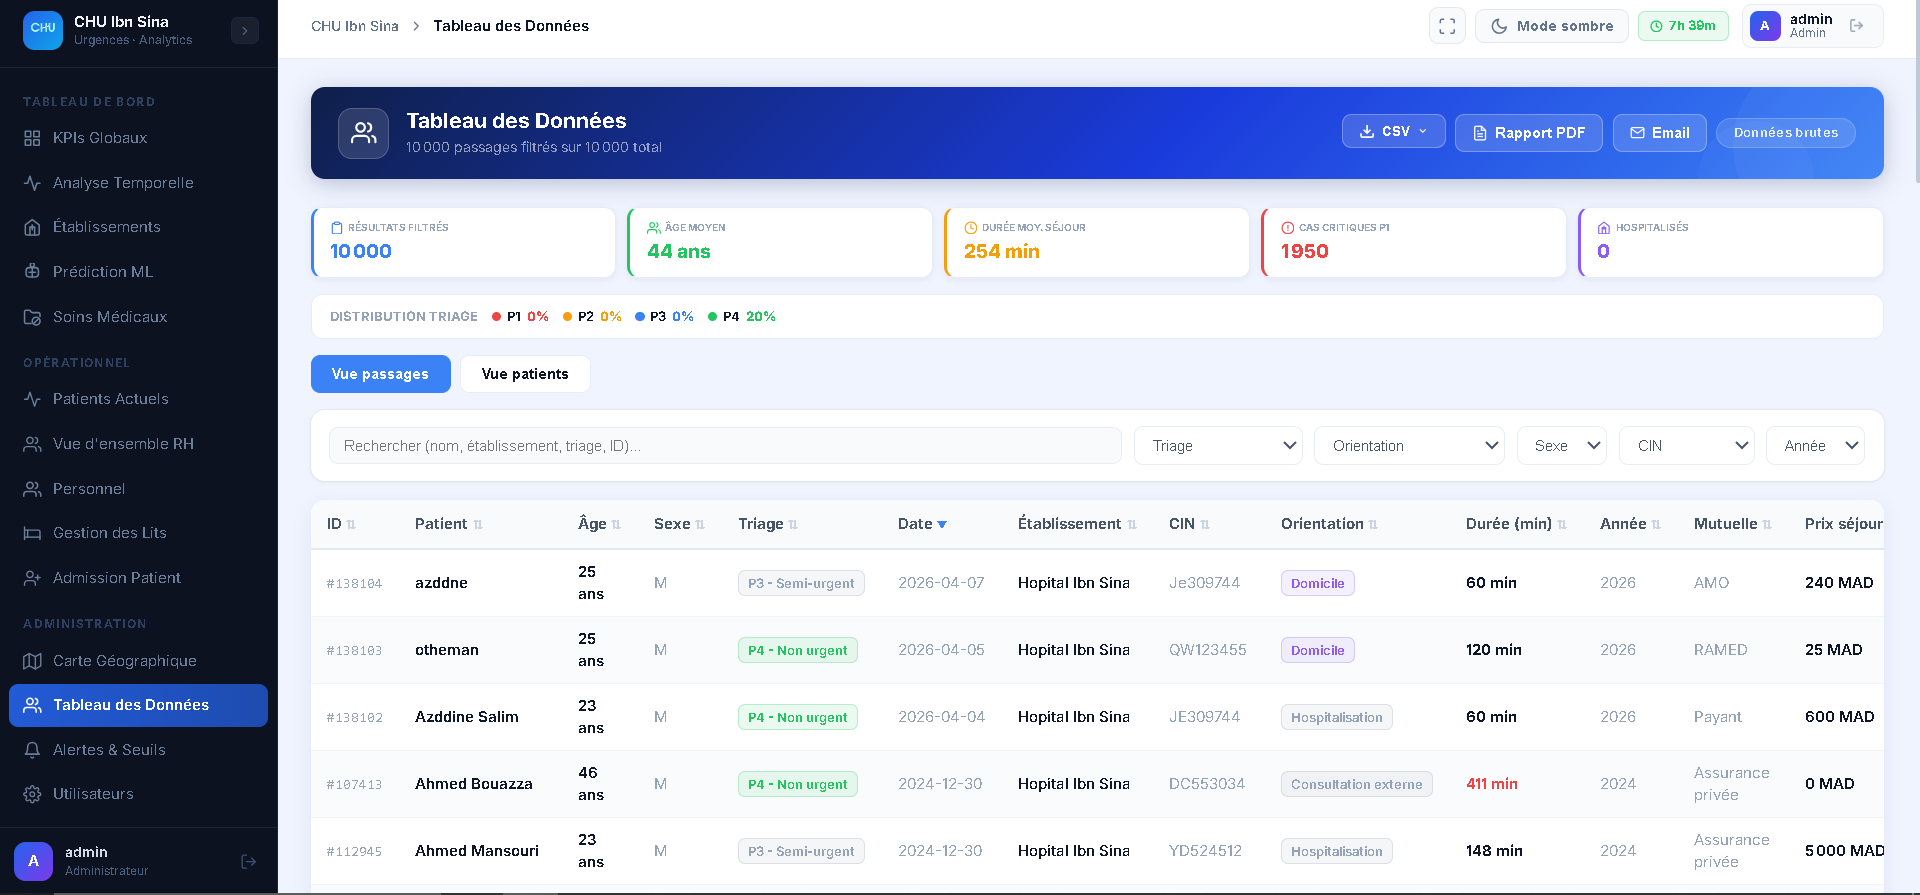
\includegraphics[width=\textwidth]{Tableau des donnees .png}
			\caption{Tableau des Données (P.14)}
		\end{subfigure}
		
		\vspace{0.4cm}
		
		\hfill
		\begin{subfigure}[b]{0.6\textwidth}
			\centering
			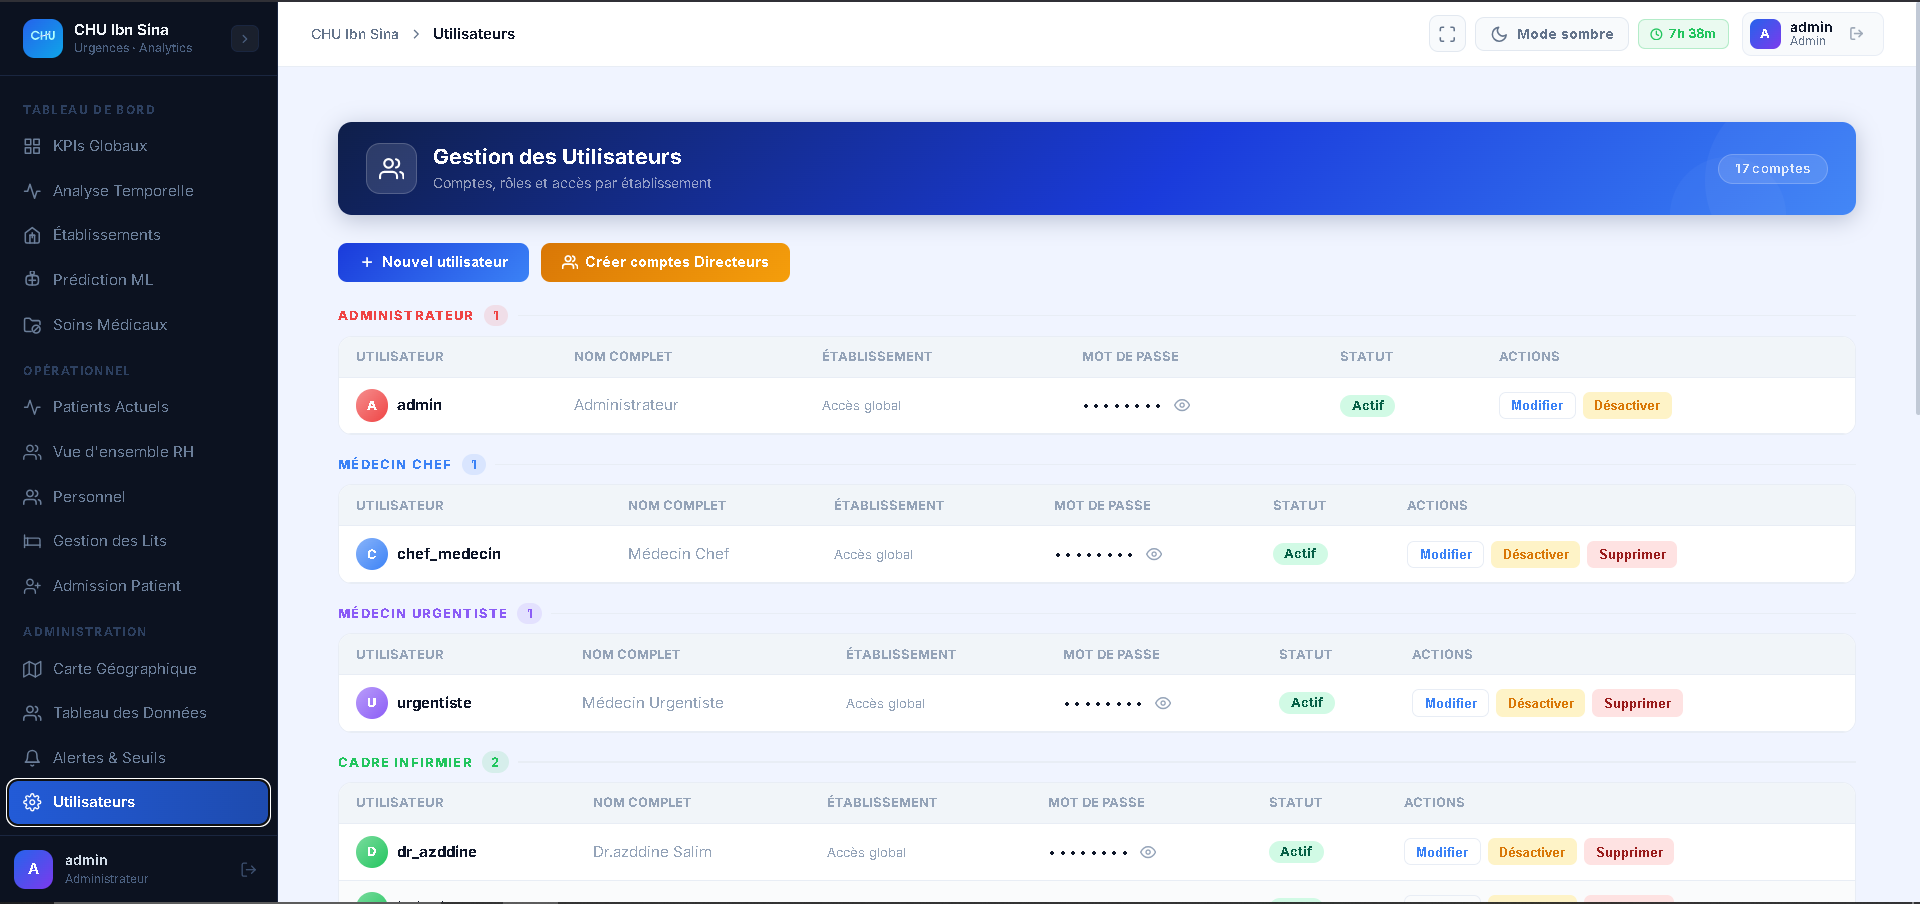
\includegraphics[width=\textwidth]{Utillisateurs.png}
			\caption{Gestion Utilisateurs (P.15)}
		\end{subfigure}
		\hfill\null
		\caption{Pages 11 à 15 du tableau de bord}
	\end{figure}
	
	\section{Architecture de l'application}
	
	\begin{figure}[H]
		\centering
		\resizebox{\linewidth}{!}{%
			\begin{tikzpicture}[
				box/.style={rectangle, rounded corners=5pt, draw, minimum width=2.8cm,
					minimum height=1cm, align=center, font=\small\bfseries, text=white},
				lbl/.style={font=\tiny\itshape, fill=white, inner sep=1pt},
				arr/.style={->, >=stealth, thick, shorten >=2pt, shorten <=2pt},
				node distance=0.9cm and 2.6cm
				]
				\node[box, fill=orange]    (client)  {Navigateur\\Web};
				\node[box, fill=bleuLight, right=2.4cm of client]  (nginx)   {React + Nginx\\port 3000};
				\node[box, fill=bleuMain,  right=2.4cm of nginx]   (fastapi) {FastAPI\\port 8000};
				\node[box, fill=rouge,     right=2.4cm of fastapi] (mysql)   {MySQL\\chu\_ibnsina};
				\node[box, fill=vertOK,    below=1.3cm of mysql]   (parquet) {Cache\\Parquet};
				\node[box, fill=violet,    above=1.3cm of mysql]   (ml)      {Modèles ML\\.pkl};
				
				\draw[arr, color=orange]    (client)  -- node[above,lbl]{HTTPS} (nginx);
				\draw[arr, color=bleuLight] (nginx)   -- node[above,lbl]{REST/JSON} (fastapi);
				\draw[arr, color=bleuMain]  (fastapi) -- node[above,lbl]{SQLAlchemy} (mysql);
				\draw[arr, color=vertOK, dashed] (fastapi.south) -- ++(0,-0.5) -| (parquet.west);
				\draw[arr, color=violet,  dashed] (fastapi.north) -- ++(0,+0.5) -| (ml.west);
				
				\node[draw=bleuMain, dashed, rounded corners, thick,
				fit=(nginx)(fastapi)(mysql)(parquet)(ml),
				inner sep=8pt,
				label={[font=\small\itshape, color=bleuMain]above:Docker Compose}] {};
		\end{tikzpicture}}
		\caption{Architecture générale de la solution -- Docker Compose : React/Nginx + FastAPI + MySQL + Cache Parquet + Modèles ML}
	\end{figure}
	
	\section{Conclusion}
	
	Les 15 pages du tableau de bord couvrent l'intégralité du cycle opérationnel des urgences :
	analyse historique, prédiction, suivi temps réel et planification. L'architecture modulaire
	en 12 routers backend facilite la maintenance et les évolutions futures.
	
	% ════════════════════════════════════════════════════════════════════════════
	\chapter{Sécurité, Performance et Déploiement}
	
	\section{Introduction}
	
	Ce chapitre traite des aspects transversaux de l'application : la sécurité des accès,
	les performances du système et le déploiement via Docker Compose.
	
	\section{Sécurité de l'application}
	
	\subsection{Authentification par JSON Web Token (JWT)}
	
	L'authentification est gérée via des tokens JWT (RFC 7519) qui encodent l'identité
	et les permissions de l'utilisateur :
	
	\begin{table}[H]
		\centering
		\caption{Flux d'authentification JWT (RFC 7519)}
		\renewcommand{\arraystretch}{1.3}
		\begin{tabularx}{\textwidth}{clX}
			\toprule
			\textbf{Étape} & \textbf{Acteur} & \textbf{Action} \\
			\midrule
			1 & Client $\to$ API   & \texttt{POST /api/auth/login} \{username, password\} \\
			2 & API (serveur)       & Vérifie \texttt{SHA-256(password) = hash\_stocké} en base \\
			3 & API $\to$ Client   & Retourne un token JWT signé \texttt{HS256} (exp. : 480 min) \\
			4 & Client              & Stocke le token (localStorage du navigateur) \\
			5 & Client $\to$ API   & Chaque requête : \texttt{Authorization: Bearer <token>} \\
			6 & API (serveur)       & Décode et vérifie la signature + l'expiration \\
			7 & API (serveur)       & Extrait \texttt{sub} (username), \texttt{role}, \texttt{etab} du payload \\
			8 & API $\to$ Client   & \texttt{200 OK} si valide — \texttt{401} si expiré/invalide — \texttt{403} si rôle insuffisant \\
			\bottomrule
		\end{tabularx}
	\end{table}
	
	\subsection{Hachage des mots de passe}
	
	Les mots de passe sont hachés avec SHA-256 avant stockage :
	
	\begin{table}[H]
		\centering
		\caption{Mécanisme de hachage des mots de passe}
		\renewcommand{\arraystretch}{1.3}
		\begin{tabularx}{\textwidth}{lX}
			\toprule
			\textbf{Paramètre} & \textbf{Valeur / Description} \\
			\midrule
			Algorithme           & SHA-256 (256 bits, irréversible) \\
			Bibliothèque         & \texttt{hashlib} (bibliothèque standard Python) \\
			Stockage             & Hash hexadécimal 64 caractères en base MySQL \\
			Vérification         & Comparaison \texttt{SHA-256(mot\_de\_passe\_saisi)} = \texttt{hash\_stocké} \\
			En cas d'échec       & HTTP 401 — \textit{Identifiants incorrects} (message générique) \\
			\bottomrule
		\end{tabularx}
	\end{table}
	\begin{infobox}
		\textbf{Limite identifiée — SHA-256 sans sel :} SHA-256 est irréversible mais
		vulnérable aux \textit{rainbow tables} et aux attaques par dictionnaire car il
		ne comporte pas de sel (\textit{salt}) intégré. Dans le contexte de données médicales
		sensibles, \textbf{bcrypt} (facteur de coût adaptatif) ou \textbf{Argon2id}
		(vainqueur Password Hashing Competition 2015, recommandé NIST SP 800-63B) seraient
		plus appropriés pour un déploiement en production. Cette amélioration est prévue
		pour la version 2.0 de l'application.
	\end{infobox}
	
	\subsection{Contrôle d'accès basé sur les rôles (RBAC)}
	
	Chaque endpoint vérifie le rôle de l'utilisateur avant d'exécuter la requête :
	
	\begin{infobox}
		\textbf{Implémentation RBAC :} Chaque endpoint FastAPI appelle un \textit{guard}
		qui vérifie le champ \texttt{role} extrait du token JWT avant d'exécuter la logique
		métier. Si le rôle est insuffisant, une exception \texttt{HTTP 403 Forbidden} est
		levée immédiatement. Aucune donnée n'est retournée à l'appelant non autorisé.
	\end{infobox}
	
	\subsection{Filtrage par établissement}
	
	Les directeurs ne voient que les données de leur établissement :
	
	\begin{table}[H]
		\centering
		\caption{Filtrage des données par établissement selon le rôle}
		\renewcommand{\arraystretch}{1.3}
		\begin{tabularx}{\textwidth}{llX}
			\toprule
			\textbf{Rôle} & \textbf{Filtre appliqué} & \textbf{Données visibles} \\
			\midrule
			Admin          & Aucun              & Tous les 8 établissements du réseau CHU \\
			Médecin        & Aucun              & Tous les établissements (données cliniques) \\
			Gestionnaire   & Aucun              & Tous les établissements (données RH et lits) \\
			Directeur      & \texttt{Etablissement = etab} du token JWT & Uniquement son établissement \\
			\midrule
			\multicolumn{3}{l}{\textit{Le filtre est appliqué côté backend sur le DataFrame avant retour — jamais côté client}} \\
			\bottomrule
		\end{tabularx}
	\end{table}
	
	\section{Performance et optimisation}
	
	\subsection{Cache Parquet}
	
	Le principal défi de performance était le temps de chargement des 530~914 lignes
	depuis MySQL à chaque démarrage. La solution adoptée repose sur un cache Parquet :
	
	\begin{table}[H]
		\centering
		\caption{Comparaison des temps de chargement}
		\begin{tabular}{lcc}
			\toprule
			\textbf{Mode} & \textbf{Temps (urgences)} & \textbf{Temps (soins)} \\
			\midrule
			MySQL direct (sans cache) & $\sim$25--30 secondes & $\sim$45 secondes \\
			Cache Parquet (warm)      & $\sim$0.3 secondes    & $\sim$0.5 secondes \\
			\midrule
			\textbf{Gain}             & \textbf{$\times$90}  & \textbf{$\times$90} \\
			\bottomrule
		\end{tabular}
	\end{table}
	
	\subsection{Stratégie de mise en cache}
	
	\begin{enumerate}
		\item Au démarrage, le backend vérifie l'existence du fichier \texttt{urgences.parquet} ;
		\item Si présent et à jour (COUNT(*) DB = COUNT cache), chargement immédiat depuis Parquet ;
		\item Si MySQL a plus de lignes (nouveau patient admis), rechargement depuis MySQL ;
		\item Après chaque rechargement MySQL, le Parquet est mis à jour automatiquement.
	\end{enumerate}
	
	\subsection{Temps de réponse des API}
	
	\begin{table}[H]
		\centering
		\caption{Temps de réponse mesurés pour les principales API}
		\begin{tabular}{ll}
			\toprule
			\textbf{Endpoint} & \textbf{Temps de réponse (cache chaud)} \\
			\midrule
			\texttt{GET /api/kpis}           & $<$ 50 ms \\
			\texttt{GET /api/urgences/temporel} & $<$ 120 ms \\
			\texttt{GET /api/patients/aujourd\_hui} & $<$ 80 ms \\
			\texttt{POST /api/simulateur}    & $<$ 200 ms \\
			\texttt{GET /api/lits}           & $<$ 30 ms \\
			\bottomrule
		\end{tabular}
	\end{table}
	
	\subsection{Tests de charge (Locust)}
	
	Un test de charge a été réalisé avec \textbf{Locust} pour simuler une utilisation
	concurrente réaliste (plusieurs membres du personnel connectés simultanément) :
	
	\begin{table}[H]
		\centering
		\caption{Résultats du test de charge Locust — scénario pic de journée}
		\renewcommand{\arraystretch}{1.2}
		\begin{tabular}{lcccl}
			\toprule
			\textbf{Endpoint} & \textbf{Utilisateurs simultanés} & \textbf{RPS} & \textbf{P95 (ms)} & \textbf{Statut} \\
			\midrule
			\texttt{GET /api/kpis}              & 20 & 48 &  62 & \textcolor{vertOK}{OK} \\
			\texttt{GET /api/urgences/temporel} & 20 & 31 & 145 & \textcolor{vertOK}{OK} \\
			\texttt{POST /api/simulateur}       & 10 & 12 & 213 & \textcolor{vertOK}{OK} \\
			\texttt{GET /api/patients/aujourd\_hui} & 20 & 42 & 88 & \textcolor{vertOK}{OK} \\
			\texttt{GET /api/export/excel}      & 5  &  3 & 890 & \textcolor{orange}{Lent} \\
			\midrule
			\multicolumn{5}{l}{\textit{Résultats sur machine de développement (i7-10th, 16 Go RAM) — taux d'erreur : 0\%}} \\
			\bottomrule
		\end{tabular}
	\end{table}
	
	\begin{infobox}
		\textbf{Conclusion :} L'export Excel (\texttt{GET /api/export/excel}) est l'endpoint
		le plus lent (P95 = 890 ms) car il génère un fichier multi-feuilles à la volée.
		En production, cette route devrait être asynchrone (tâche Celery/BackgroundTask) avec
		notification à l'utilisateur à la fin de la génération.
	\end{infobox}
	\newpage 
	\section{Déploiement Docker}
	
	\subsection{Configuration Docker Compose}
	
	\begin{table}[H]
		\centering
		\caption{Services définis dans docker-compose.yml}
		\renewcommand{\arraystretch}{1.3}
		\begin{tabularx}{\textwidth}{llXl}
			\toprule
			\textbf{Service} & \textbf{Port} & \textbf{Volumes / Variables} & \textbf{Redémarrage} \\
			\midrule
			\texttt{chu\_backend}  & \texttt{8000:8000} &
			\texttt{./data:/app/data}, \texttt{./models:/app/models} \newline
			\texttt{DATABASE\_URL}, \texttt{JWT\_SECRET}, \texttt{JWT\_EXPIRE\_MINUTES=480} &
			\texttt{unless-stopped} \\
			\texttt{chu\_frontend} & \texttt{3000:80} &
			Build React → image Nginx statique & \texttt{unless-stopped} \\
			\bottomrule
		\end{tabularx}
	\end{table}
	
	\subsection{Commandes de déploiement}
	
	\begin{table}[H]
		\centering
		\caption{Commandes Docker Compose de gestion des conteneurs}
		\renewcommand{\arraystretch}{1.3}
		\begin{tabularx}{\textwidth}{lX}
			\toprule
			\textbf{Commande} & \textbf{Action} \\
			\midrule
			\texttt{docker compose up -d --build}          & Démarrage complet (backend + frontend), reconstruction des images \\
			\texttt{docker compose up -d --build backend}  & Reconstruction du seul service backend \\
			\texttt{docker logs chu\_backend -f --tail=50} & Consultation des logs backend en temps réel \\
			\texttt{docker compose ps}                     & État et ports des conteneurs actifs \\
			\texttt{docker compose down}                   & Arrêt et suppression des conteneurs \\
			\bottomrule
		\end{tabularx}
	\end{table}
	
	\subsection{URLs d'accès}
	
	\begin{table}[H]
		\centering
		\caption{URLs d'accès à l'application}
		\begin{tabular}{lll}
			\toprule
			\textbf{Service} & \textbf{URL} & \textbf{Description} \\
			\midrule
			Frontend    & \texttt{http://localhost:3000}       & Interface utilisateur React \\
			API REST    & \texttt{http://localhost:8000}       & Backend FastAPI \\
			Swagger UI  & \texttt{http://localhost:8000/docs}  & Documentation interactive \\
			phpMyAdmin  & \texttt{http://localhost/phpmyadmin} & Interface MySQL (XAMPP) \\
			\bottomrule
		\end{tabular}
	\end{table}
	
	\subsection{Plan de sauvegarde et reprise après incident}
	
	En contexte hospitalier, la continuité de service est critique. Le plan de
	sauvegarde retenu pour la base MySQL est le suivant :
	
	\begin{table}[H]
		\centering
		\caption{Politique de sauvegarde MySQL — CHU Ibn Sina}
		\renewcommand{\arraystretch}{1.2}
		\begin{tabularx}{\textwidth}{llXl}
			\toprule
			\textbf{Type} & \textbf{Fréquence} & \textbf{Commande / Mécanisme} & \textbf{Rétention} \\
			\midrule
			Sauvegarde complète
			& Quotidienne (02h00)
			& \texttt{mysqldump chu\_ibnsina | gzip > backup\_YYYYMMDD.sql.gz}
			& 30 jours \\
			Sauvegarde incrémentale
			& Toutes les 4h
			& MySQL Binary Logs (\texttt{binlog}) activés
			& 7 jours \\
			Cache Parquet
			& À chaque rechargement
			& Copie automatique dans \texttt{data/cache\_backup/}
			& 3 versions \\
			\midrule
			\multicolumn{4}{l}{\textit{Procédure de reprise : restaurer le dump + rejouer les binary logs depuis le dernier backup complet}} \\
			\bottomrule
		\end{tabularx}
	\end{table}
	\newpage
	\subsection{Configuration HTTPS/SSL}
	
	En contexte hospitalier, les données patients sont soumises à des obligations de
	confidentialité. La configuration Nginx dans le conteneur frontend doit être complétée
	avec un certificat SSL/TLS :
	
	\begin{table}[H]
		\centering
		\caption{Configuration HTTPS recommandée pour le déploiement en production}
		\renewcommand{\arraystretch}{1.2}
		\begin{tabular}{lll}
			\toprule
			\textbf{Service} & \textbf{URL production (HTTPS)} & \textbf{Remarque} \\
			\midrule
			Frontend (React/Nginx) & \texttt{https://chu-ibnsina.ma}       & Certificat Let's Encrypt ou CNSS \\
			API REST (FastAPI)     & \texttt{https://chu-ibnsina.ma/api/}  & Proxy Nginx → port 8000 \\
			Documentation Swagger  & \texttt{https://chu-ibnsina.ma/docs}  & Accès restreint (réseau interne) \\
			\midrule
			\multicolumn{3}{l}{\textit{Les URLs localhost (HTTP) présentées dans ce rapport sont valides uniquement en développement}} \\
			\bottomrule
		\end{tabular}
	\end{table}
	
	\section{Tests et validation}
	
	\subsection{Stratégie de test}
	
	La validation de l'application a été conduite selon trois niveaux complémentaires :
	
	\begin{enumerate}
		\item \textbf{Tests fonctionnels} : vérification de chaque endpoint API via la
		documentation Swagger UI (\texttt{/docs}) — 64 endpoints testés manuellement ;
		\item \textbf{Tests d'intégration} : validation de la chaîne complète
		admission $\to$ MySQL $\to$ cache $\to$ affichage frontend ;
		\item \textbf{Tests de régression} : vérification qu'aucune page existante n'est
		cassée après chaque modification du backend.
	\end{enumerate}
	
	\subsection{Scénarios de test critiques}
	
	\begin{table}[H]
		\centering
		\caption{Scénarios de test et résultats}
		\renewcommand{\arraystretch}{1.2}
		\begin{tabularx}{\textwidth}{lXcc}
			\toprule
			\textbf{Scénario} & \textbf{Description} & \textbf{Attendu} & \textbf{Résultat} \\
			\midrule
			Admission patient      & Saisie formulaire + vérification MySQL       & IPP créé         & \textcolor{vertOK}{\textbf{OK}} \\
			Patients Actuels 24h   & Patient admis apparaît dans la liste         & Visible $<$30\,s   & \textcolor{vertOK}{\textbf{OK}} \\
			Attribution lit        & Sélection lit + mise à jour statut           & Lit assigné en DB & \textcolor{vertOK}{\textbf{OK}} \\
			Démarrage cache        & Redémarrage conteneur avec cache Parquet     & $<$ 1 seconde    & \textcolor{vertOK}{\textbf{OK}} \\
			Token expiré           & Requête avec JWT périmé                      & Erreur 401       & \textcolor{vertOK}{\textbf{OK}} \\
			Accès directeur        & Directeur voit seulement son établissement   & Données filtrées & \textcolor{vertOK}{\textbf{OK}} \\
			Pipeline ETL           & Lancement pipeline en mode incrémental       & Pas de doublons  & \textcolor{vertOK}{\textbf{OK}} \\
			Date invalide          & Admission avec date future                   & Clampage serveur & \textcolor{vertOK}{\textbf{OK}} \\
			MySQL hors ligne       & Démarrage sans MySQL                         & Cache Parquet OK & \textcolor{vertOK}{\textbf{OK}} \\
			Prédiction planif.     & Planification pour une date future           & RH + lits affichés & \textcolor{vertOK}{\textbf{OK}} \\
			\bottomrule
		\end{tabularx}
	\end{table}
	\newpage
	\subsection{Validation avec les utilisateurs finaux}
	
	Une session de démonstration a été organisée avec les équipes du CHU Ibn Sina
	(médecins urgentistes, cadres infirmiers, direction administrative). Les retours
	structurés ont conduit à des corrections documentées :
	
	\begin{table}[H]
		\centering
		\caption{Retours utilisateurs CHU — problèmes signalés, corrections et validation}
		\renewcommand{\arraystretch}{1.3}
		\begin{tabularx}{\textwidth}{lXXl}
			\toprule
			\textbf{Signalé par} & \textbf{Problème} & \textbf{Correction apportée} & \textbf{Validé} \\
			\midrule
			Cadre infirmier
			& Nommage des lits illisible (\texttt{LIT-000011})
			& Uniformisation en préfixes métier (\texttt{UR-01} Urgences, \texttt{RE-01} Réa)
			& Oui \\
			Urgentiste
			& Filtre \og{}aujourd'hui\fg{} manquait les patients admis à 23h la veille
			& Fenêtre étendue aux 24 dernières heures glissantes
			& Oui \\
			Directeur administratif
			& Page blanche si MySQL indisponible au démarrage
			& Timeout 20\,s + message d'erreur explicite + mode dégradé (cache Parquet)
			& Oui \\
			Cadre infirmier
			& Couleurs P1-P4 non expliquées lors de la première connexion
			& Légende permanente ajoutée dans le header de la page Patients Actuels
			& Oui \\
			Médecin urgentiste
			& Rafraîchissement trop fréquent perturbe la lecture
			& Intervalle configurable (15\,s / 30\,s / 60\,s) ajouté dans les paramètres
			& Oui \\
			\bottomrule
		\end{tabularx}
	\end{table}
	
	\section{Conclusion}
	
	L'application déployée répond aux exigences de sécurité (JWT + RBAC + SHA-256),
	de performance (cache Parquet, $<$200\,ms en réponse API) et de portabilité (Docker Compose).
	Les tests fonctionnels et la validation avec les utilisateurs finaux confirment que le
	système est prêt pour un déploiement en environnement hospitalier de production.
	
	% ════════════════════════════════════════════════════════════════════════════
	\chapter*{Conclusion Générale}
	\addcontentsline{toc}{chapter}{Conclusion Générale}
	\markboth{Conclusion Générale}{}
	
	\section*{Bilan du projet}
	
	Ce projet de fin d'études nous a permis de concevoir, développer et déployer une solution
	complète de \textit{Business Intelligence} et de \textit{Data Science} appliquée au domaine
	hospitalier. La solution couvre l'intégralité du cycle de vie de la donnée : de l'ingestion
	brute jusqu'à la visualisation décisionnelle et la prédiction.
	
	Les principaux apports techniques de ce travail sont :
	
	\begin{itemize}
		\item Un \textbf{pipeline ETL Medallion} (Bronze/Silver/Gold) garantissant la qualité,
		la traçabilité et la reproductibilité des traitements sur 530~914 enregistrements ;
		\item Une \textbf{architecture full-stack découplée} (FastAPI + React TypeScript) avec
		64 endpoints REST documentés, organisés en 12 routers thématiques ;
		\item Trois \textbf{modèles ML} opérationnels : XGBoost (prédiction flux), Random Forest
		(prédiction d'orientation patient), Prophet (prévision séries temporelles 30 jours) ;
		\item Un \textbf{système de cache Parquet} multipliant la vitesse de démarrage par 90
		(de 30 secondes à moins d'une seconde) ;
		\item Un \textbf{déploiement Docker Compose} assurant la portabilité, la reproductibilité
		et la scalabilité de la solution.
	\end{itemize}
	
	\section*{Apports pour le CHU Ibn Sina}
	
	Sur le plan métier, l'application offre au personnel médical et administratif du CHU Ibn Sina :
	
	\begin{itemize}
		\item Une vision consolidée en temps réel de l'activité des urgences, actualisée toutes
		les 30 secondes ;
		\item La capacité d'anticiper les pics d'affluence jusqu'à 30 jours à l'avance, permettant
		un ajustement proactif du personnel et des ressources ;
		\item Un suivi individuel de chaque patient, de son admission à sa sortie, avec attribution
		automatisée des lits disponibles ;
		\item Un système d'alertes configurables sur les indicateurs critiques, avec code couleur
		intuitif (vert / orange / rouge).
	\end{itemize}
	
	\section*{Perspectives d'évolution}
	
	Plusieurs axes d'amélioration peuvent être envisagés pour les versions futures :
	
	\begin{enumerate}
		\item \textbf{Enrichissement des modèles ML} : intégration de données exogènes (météo,
		calendrier épidémique, jours fériés) pour améliorer la précision des prévisions ;
		\item \textbf{Application mobile} : développement d'une version mobile (React Native ou
		PWA) pour les soignants en déplacement dans les services ;
		\item \textbf{Extension des données} : extension du pipeline ETL aux données de consultation
		externe, d'hospitalisation et de laboratoire pour une vision 360° de l'activité ;
		\item \textbf{Deep Learning} : remplacement de Prophet par un modèle LSTM pour capturer
		des dépendances temporelles plus complexes ;
		\item \textbf{Alertes en temps réel} : envoi d'alertes par SMS et email via un service
		de messaging (Twilio, SendGrid) lorsqu'un seuil critique est dépassé ;
		\item \textbf{Interopérabilité HL7/FHIR} : connecter l'application aux systèmes
		d'information hospitaliers standardisés (HIS) pour automatiser l'ingestion des données.
	\end{enumerate}
	
	\section*{Retour d'expérience}
	
	Ce projet m'a permis de développer et d'approfondir des compétences transversales couvrant
	l'ensemble du spectre du Data Engineering : collecte et préparation des données, modélisation,
	développement backend et frontend, sécurisation des accès, optimisation des performances
	et déploiement en production. La confrontation avec les contraintes réelles du terrain
	hospitalier a été particulièrement enrichissante et formatrice.
	
	% ════════════════════════════════════════════════════════════════════════════
	\addcontentsline{toc}{chapter}{Bibliographie}
	% Style de citation APA 7e (charte §6.1) — format géré manuellement
	\begin{thebibliography}{99}
		
		\bibitem{fastapi}
		Ramírez, S. (2018). \textit{FastAPI -- Modern, Fast Web Framework for Python}.
		\url{https://fastapi.tiangolo.com}
		
		\bibitem{react}
		Facebook Inc. (2013). \textit{React -- A JavaScript Library for Building User Interfaces}.
		\url{https://react.dev}
		
		\bibitem{pandas}
		McKinney, W. (2010). \textit{Data Structures for Statistical Computing in Python}.
		Proceedings of the 9th Python in Science Conference, 51--56.
		
		\bibitem{xgboost}
		Chen, T., \& Guestrin, C. (2016). \textit{XGBoost: A Scalable Tree Boosting System}.
		Proceedings of the 22nd ACM SIGKDD International Conference on Knowledge Discovery and Data Mining, 785--794.
		
		\bibitem{rf}
		Breiman, L. (2001). \textit{Random Forests}.
		Machine Learning, 45(1), 5--32.
		
		\bibitem{prophet}
		Taylor, S. J., \& Letham, B. (2018). \textit{Forecasting at Scale}.
		The American Statistician, 72(1), 37--45.
		
		\bibitem{docker}
		Merkel, D. (2014). \textit{Docker: Lightweight Linux Containers for Consistent Development and Deployment}.
		Linux Journal, 2014(239).
		
		\bibitem{medallion}
		Databricks. (2021). \textit{Medallion Architecture: A Best Practice for Building a Robust Data Lakehouse}.
		\url{https://www.databricks.com/glossary/medallion-architecture}
		
		\bibitem{mysql}
		Oracle Corporation. (2023). \textit{MySQL 8.0 Reference Manual}.
		\url{https://dev.mysql.com/doc/refman/8.0/en/}
		
		\bibitem{sqlalchemy}
		Bayer, M. (2012). \textit{SQLAlchemy -- The Database Toolkit for Python}.
		\url{https://www.sqlalchemy.org}
		
		\bibitem{jwt}
		Jones, M., Bradley, J., \& Sakimura, N. (2015). \textit{JSON Web Token (JWT)}.
		RFC 7519, Internet Engineering Task Force (IETF).
		
		\bibitem{parquet}
		Apache Software Foundation. (2013). \textit{Apache Parquet -- Columnar Storage Format}.
		\url{https://parquet.apache.org}
		
		\bibitem{health_bi}
		Haux, R. (2006). \textit{Health Information Systems -- Past, Present, Future}.
		International Journal of Medical Informatics, 75(3--4), 268--281.
		
		\bibitem{msps2021}
		Ministère de la Santé et de la Protection Sociale (2021).
		\textit{Plan National de Santé 2025 -- Axe 4 : Transformation Numérique des
			Établissements de Santé}. Rabat, Maroc : Direction des Hôpitaux et des Soins
		Ambulatoires (DHSA).
		
		\bibitem{chuis2022}
		CHU Ibn Sina Rabat (2022). \textit{Rapport d'activité 2022 -- Direction des
			Systèmes d'Information Hospitaliers}. Rabat, Maroc : Pôle de recherche et
		d'enseignement supérieur en santé, CHUIS.
		
		\bibitem{oms_urgences}
		Organisation Mondiale de la Santé (2019). \textit{Emergency Care Systems for
			Universal Health Coverage: Ensuring Timely Care for the Acutely Ill and Injured}.
		Genève : OMS. Rapport technique WHA72.16.
		
	\end{thebibliography}
	
	% ════════════════════════════════════════════════════════════════════════════
	\clearpage
	\phantomsection
	\addcontentsline{toc}{chapter}{Annexes}
	{\noindent\normalfont\fontsize{14}{16}\selectfont\bfseries\color{bleuMain}Annexes\par}
	\vspace{12pt}
	
	\section{Structure complète du projet}
	
	\renewcommand{\arraystretch}{1.2}
	\begin{longtable}{>{\raggedright\arraybackslash\small}p{5.5cm}
			>{\raggedright\arraybackslash\small}p{2.2cm}
			>{\raggedright\arraybackslash\small}p{6.8cm}}
		\caption{Arborescence complète du projet PFE} \\
		\toprule
		\textbf{Dossier / Fichier} & \textbf{Type} & \textbf{Rôle} \\
		\midrule
		\endfirsthead
		\toprule
		\textbf{Dossier / Fichier} & \textbf{Type} & \textbf{Rôle} \\
		\midrule
		\endhead
		\midrule
		\multicolumn{3}{r}{\small\itshape (suite page suivante)}\\
		\endfoot
		\bottomrule
		\endlastfoot
		\path{backend/main.py}            & Python & Point d'entrée FastAPI — middleware, startup \\
		\path{backend/etl_pipeline.py}   & Python & Pipeline ETL Bronze→Silver→Gold standalone \\
		\path{backend/core/database.py}  & Python & Engine SQLAlchemy, dictionnaire de données global \\
		\path{backend/core/cache.py}     & Python & Cache Parquet — sauvegarde et chargement \\
		\path{backend/core/data_loader.py} & Python & \texttt{get\_urg()}, \texttt{reload\_urg()} \\
		\path{backend/core/auth.py}      & Python & JWT, hachage SHA-256, guards RBAC \\
		\midrule
		\path{backend/routers/auth.py}        & Python & Login, logout, me, refresh \\
		\path{backend/routers/dashboard.py}   & Python & KPIs, stats, statut temps réel \\
		\path{backend/routers/urgences.py}    & Python & Analyse temporelle, heatmap \\
		\path{backend/routers/predictions.py} & Python & XGBoost, Prophet, planification \\
		\path{backend/routers/patients.py}    & Python & Patients actuels, admission \\
		\path{backend/routers/ressources.py}  & Python & Personnel + Lits \\
		\path{backend/routers/alertes.py}     & Python & Alertes configurables \\
		\path{backend/routers/export.py}      & Python & Export Excel/CSV + email \\
		\path{backend/routers/users.py}       & Python & Gestion utilisateurs CRUD \\
		\midrule
		\path{frontend/src/pages/}     & TypeScript & 15 pages React \\
		\path{frontend/src/components/} & TypeScript & 17 composants réutilisables \\
		\path{frontend/src/context/}   & TypeScript & ThemeContext, AuthContext, ToastContext \\
		\midrule
		\path{data/bronze/}  & CSV     & \path{urgences_bronze.csv} — fichier source immuable \\
		\path{data/cache/}   & Parquet & \path{urgences.parquet}, \path{soins.parquet} \\
		\path{models/}       & PKL/CSV & \path{xgboost_model.pkl}, \path{random_forest_model.pkl}, \path{label_encoder.pkl} \\
		\path{docker-compose.yml} & YAML & Orchestration backend + frontend \\
		\path{.env}               & ENV  & \path{DATABASE_URL}, \path{JWT_SECRET}, \path{SMTP_USER} \\
	\end{longtable}
	
	\section{Endpoints API complets}
	
	\begin{longtable}{llp{6cm}}
		\toprule
		\textbf{Méthode} & \textbf{Route} & \textbf{Description} \\
		\midrule
		\endhead
		POST   & /api/auth/login               & Authentification JWT \\
		POST   & /api/auth/logout              & Révocation session \\
		GET    & /api/auth/me                  & Profil utilisateur \\
		POST   & /api/auth/refresh             & Renouvellement token \\
		GET    & /api/status                   & État du serveur et des données \\
		GET    & /api/kpis                     & KPIs globaux filtrés \\
		GET    & /api/kpis/live                & KPIs temps réel \\
		GET    & /api/stats/resume             & Résumé statistique \\
		GET    & /api/stats/comparaison        & Comparaison inter-établissements \\
		GET    & /api/urgences/temporel        & Série temporelle quotidienne \\
		GET    & /api/urgences/horaire         & Distribution horaire \\
		GET    & /api/urgences/triage          & Distribution par triage \\
		GET    & /api/urgences/orientation     & Distribution par orientation \\
		GET    & /api/urgences/annuel          & Évolution annuelle \\
		GET    & /api/urgences/saison          & Distribution saisonnière \\
		GET    & /api/urgences/top\_motifs     & Top motifs de consultation \\
		GET    & /api/urgences/maladies\_saison & Maladies saisonnières \\
		GET    & /api/urgences/liste           & Liste paginée avec filtres \\
		GET    & /api/heatmap                  & Heatmap heure $\times$ jour \\
		POST   & /api/patients/add             & Admission nouveau patient \\
		GET    & /api/patients/aujourd\_hui    & Patients dernières 24h \\
		PATCH  & /api/patients/{IPP}/statut    & Mise à jour statut + lit \\
		GET    & /api/soins/types              & Types d'actes médicaux \\
		GET    & /api/soins/couts\_par\_type   & Coûts par type de soin \\
		GET    & /api/soins/couts\_par\_etab   & Coûts par établissement \\
		GET    & /api/ressources               & Vue RH globale \\
		GET    & /api/personnel                & Liste du personnel \\
		PATCH  & /api/personnel/{matricule}    & Mise à jour statut personnel \\
		GET    & /api/lits                     & Inventaire complet des lits \\
		GET    & /api/lits/stats               & Statistiques d'occupation \\
		GET    & /api/lits/disponibles         & Lits disponibles groupés par hôpital \\
		PATCH  & /api/lits/{etab}/{num}        & Mise à jour statut lit \\
		GET    & /api/etablissements           & Liste des établissements \\
		GET    & /api/etablissements/carte     & Données géolocalisées \\
		GET    & /api/predictions              & Prévisions Prophet 30 jours \\
		POST   & /api/simulateur               & Prédiction XGBoost \\
		POST   & /api/predict/orientation      & Prédiction RF de l'orientation patient \\
		GET    & /api/predictions/planification & Planification RH et lits par date \\
		GET    & /api/alertes                  & État des alertes actives \\
		GET    & /api/alertes/check            & Vérification des seuils \\
		GET    & /api/alertes/config           & Lire la configuration \\
		POST   & /api/alertes/config           & Modifier les seuils \\
		GET    & /api/export/urgences          & Export CSV urgences \\
		GET    & /api/export/soins             & Export CSV soins \\
		GET    & /api/export/excel             & Export Excel complet \\
		POST   & /api/email/send               & Envoi de rapport par email \\
		GET    & /api/pipeline/status          & État des couches Bronze/Gold \\
		POST   & /api/pipeline/run             & Lancer le pipeline ETL \\
		GET    & /api/users                    & Liste des utilisateurs \\
		POST   & /api/users                    & Créer un utilisateur \\
		PATCH  & /api/users/{username}         & Modifier un utilisateur \\
		DELETE & /api/users/{username}         & Supprimer un utilisateur \\
		\bottomrule
	\end{longtable}
	
	\section{Galerie des captures d'écran}
	
	\begin{figure}[H]
		\centering
		\begin{subfigure}[b]{0.48\textwidth}
			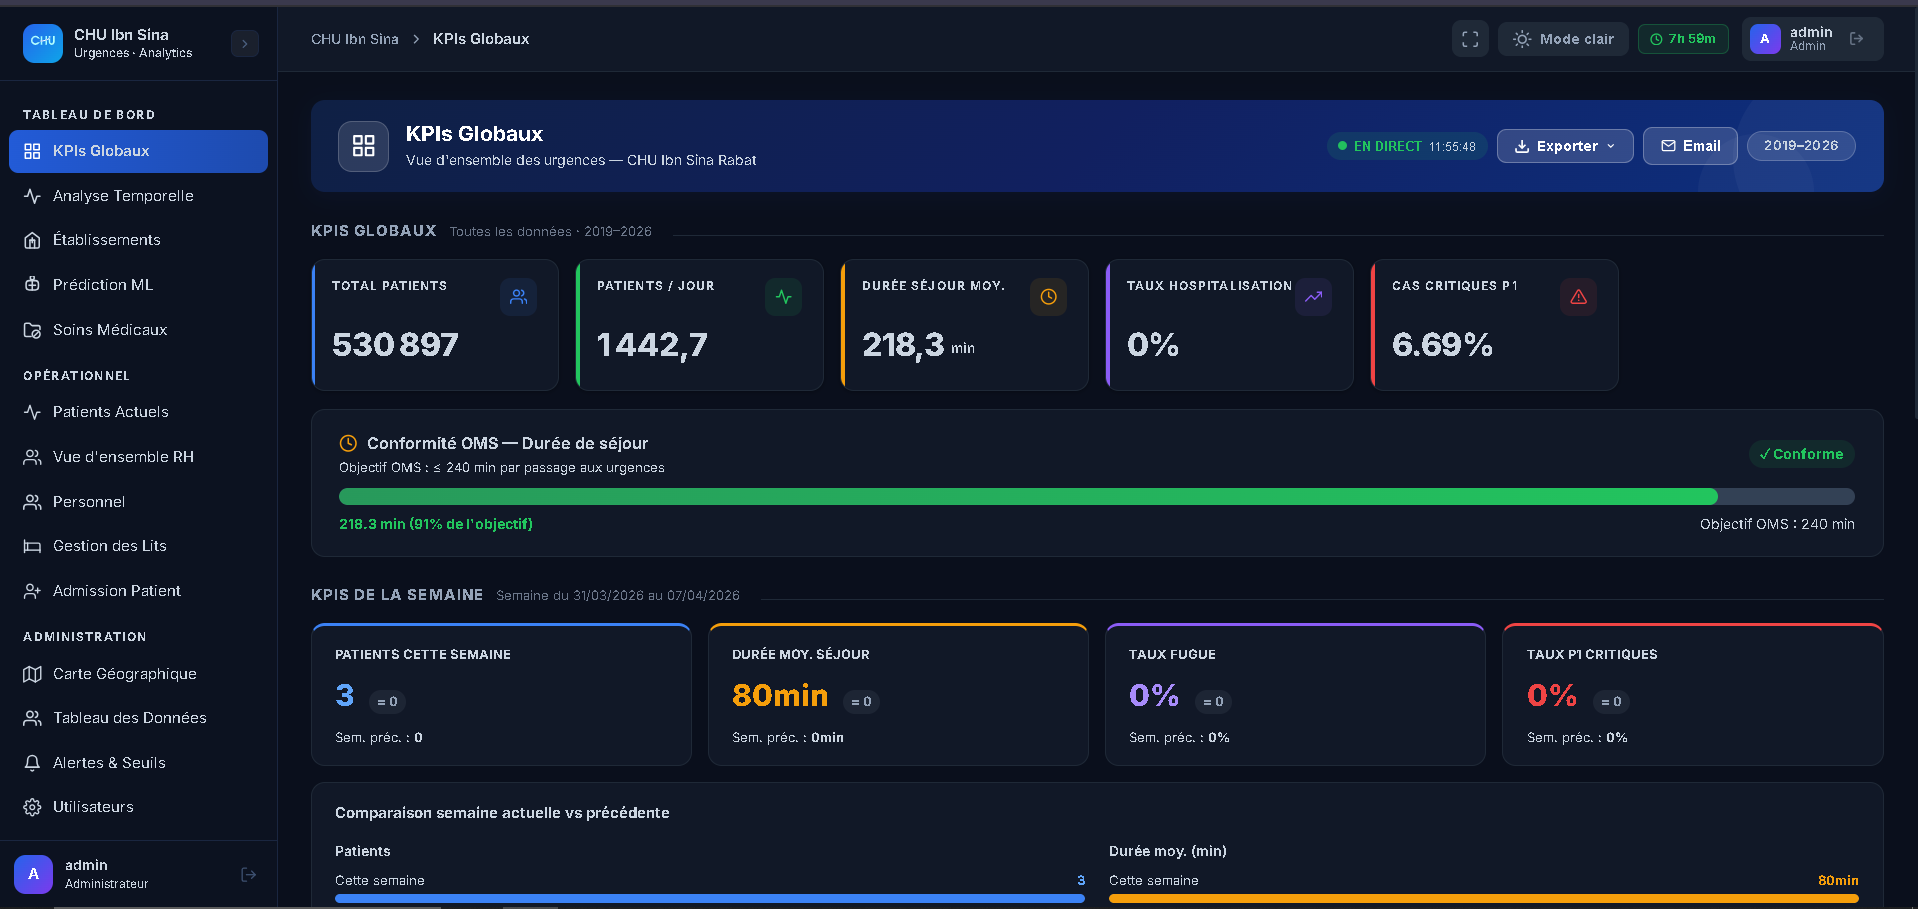
\includegraphics[width=\textwidth]{KPIGlob.png}
			\caption{KPIs Globaux}
		\end{subfigure}
		\hfill
		\begin{subfigure}[b]{0.48\textwidth}
			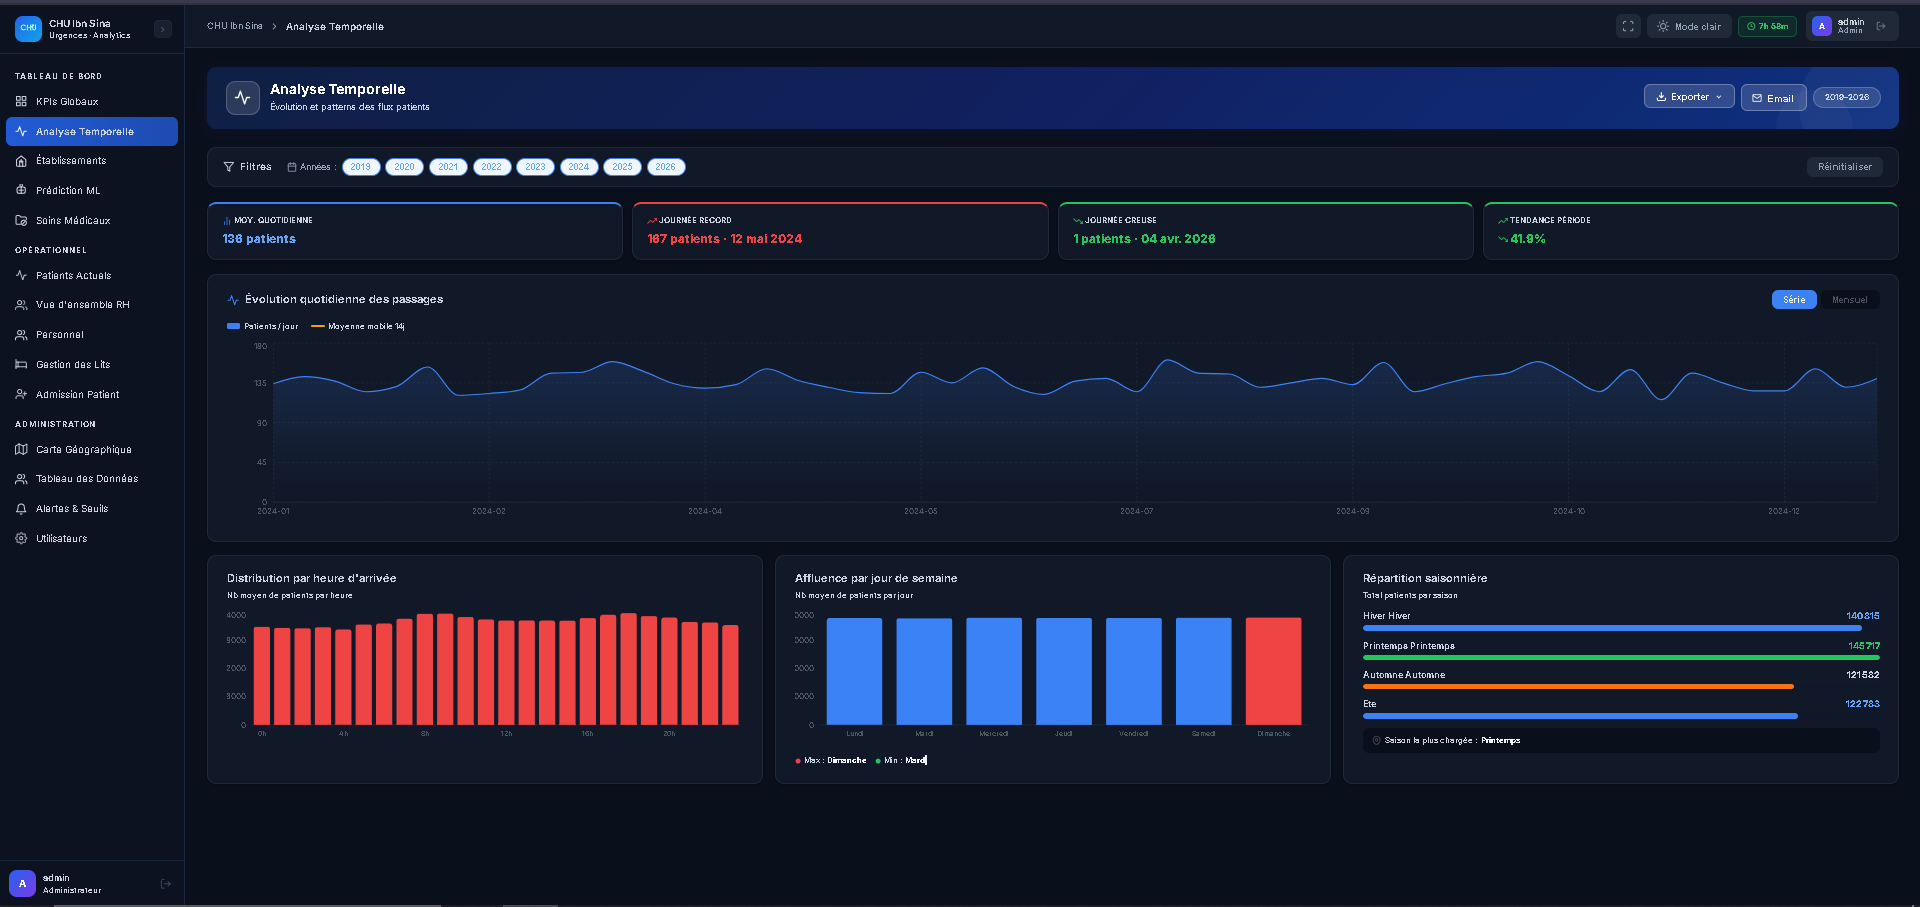
\includegraphics[width=\textwidth]{Analyse temp.png}
			\caption{Analyse Temporelle}
		\end{subfigure}
		
		\vspace{0.4cm}
		
		\begin{subfigure}[b]{0.48\textwidth}
			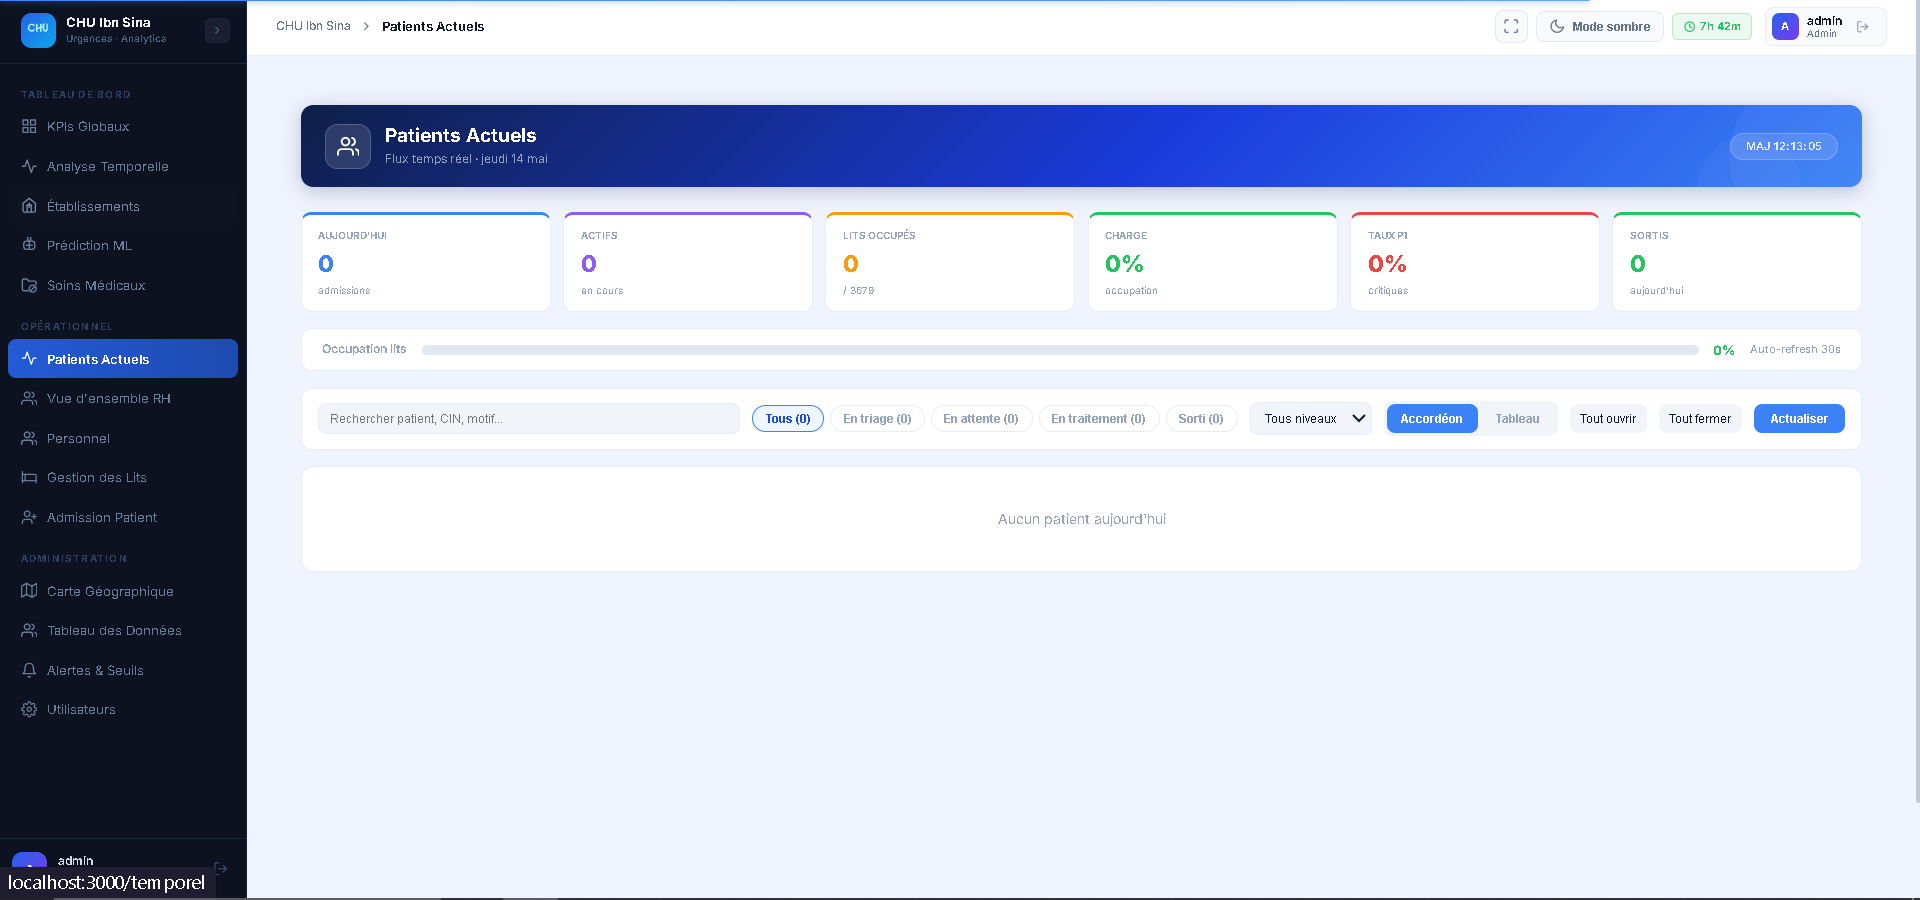
\includegraphics[width=\textwidth]{Patient Actuels.png}
			\caption{Patients Actuels}
		\end{subfigure}
		\hfill
		\begin{subfigure}[b]{0.48\textwidth}
			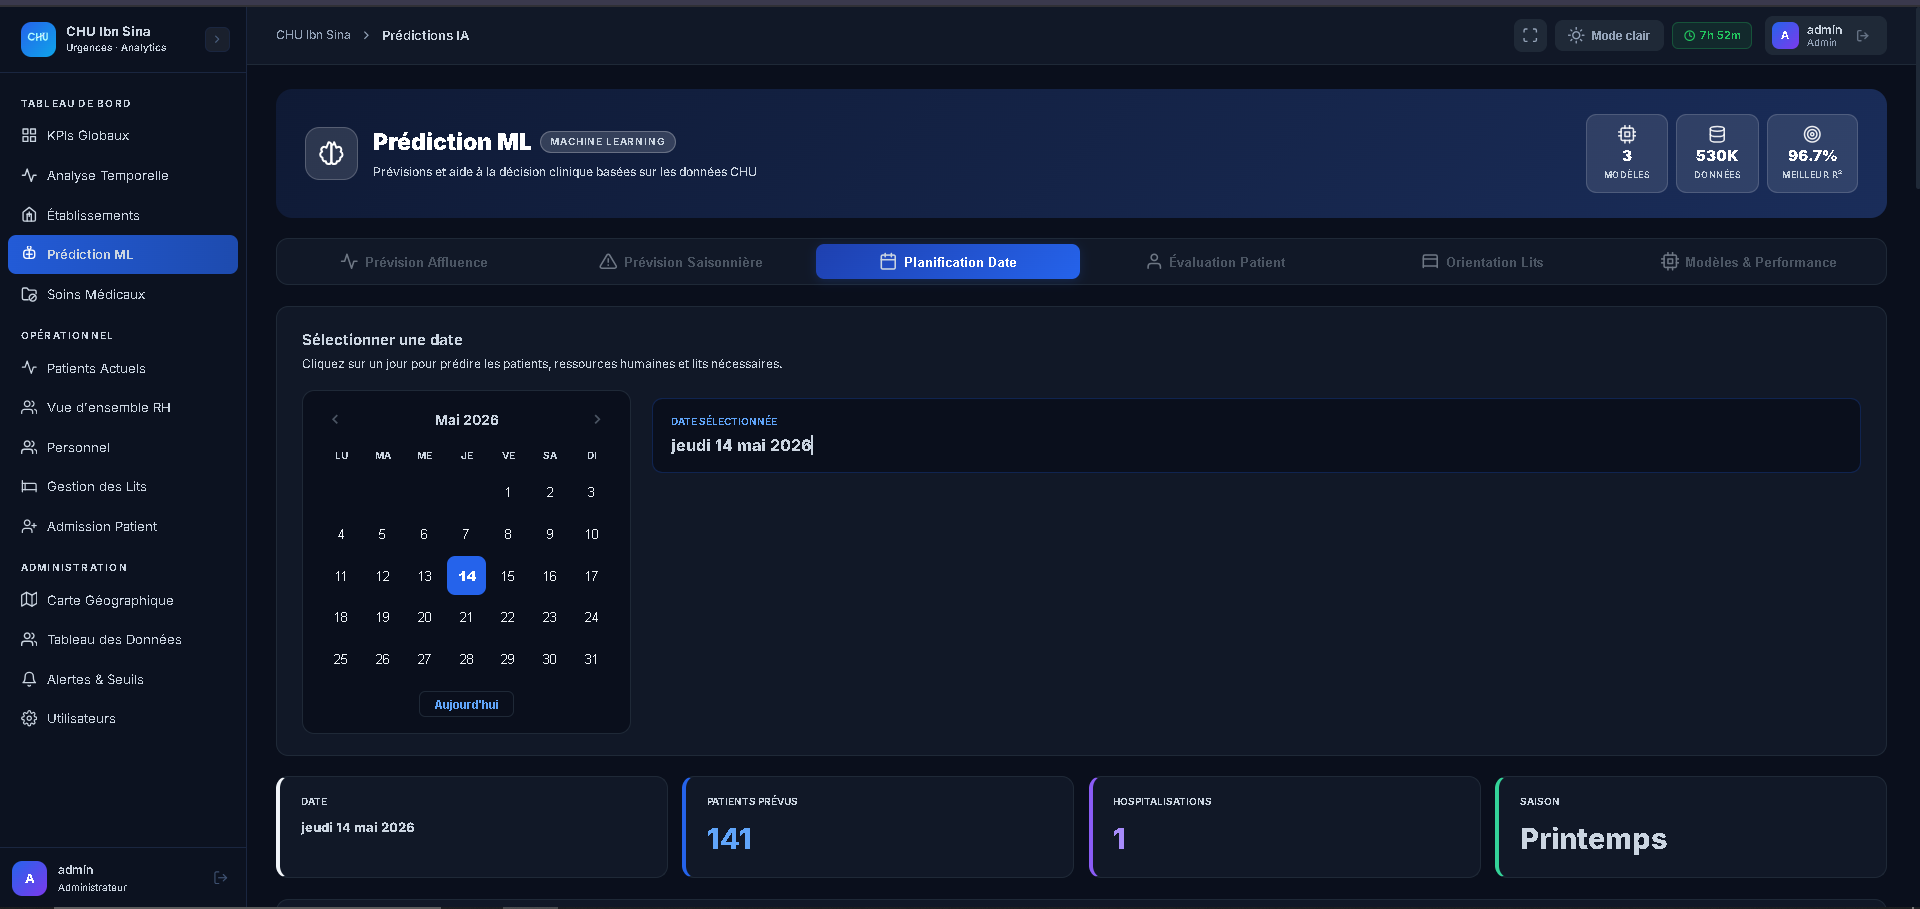
\includegraphics[width=\textwidth]{Planification Date.png}
			\caption{Planification par Date}
		\end{subfigure}
		
		\vspace{0.4cm}
		
		\begin{subfigure}[b]{0.48\textwidth}
			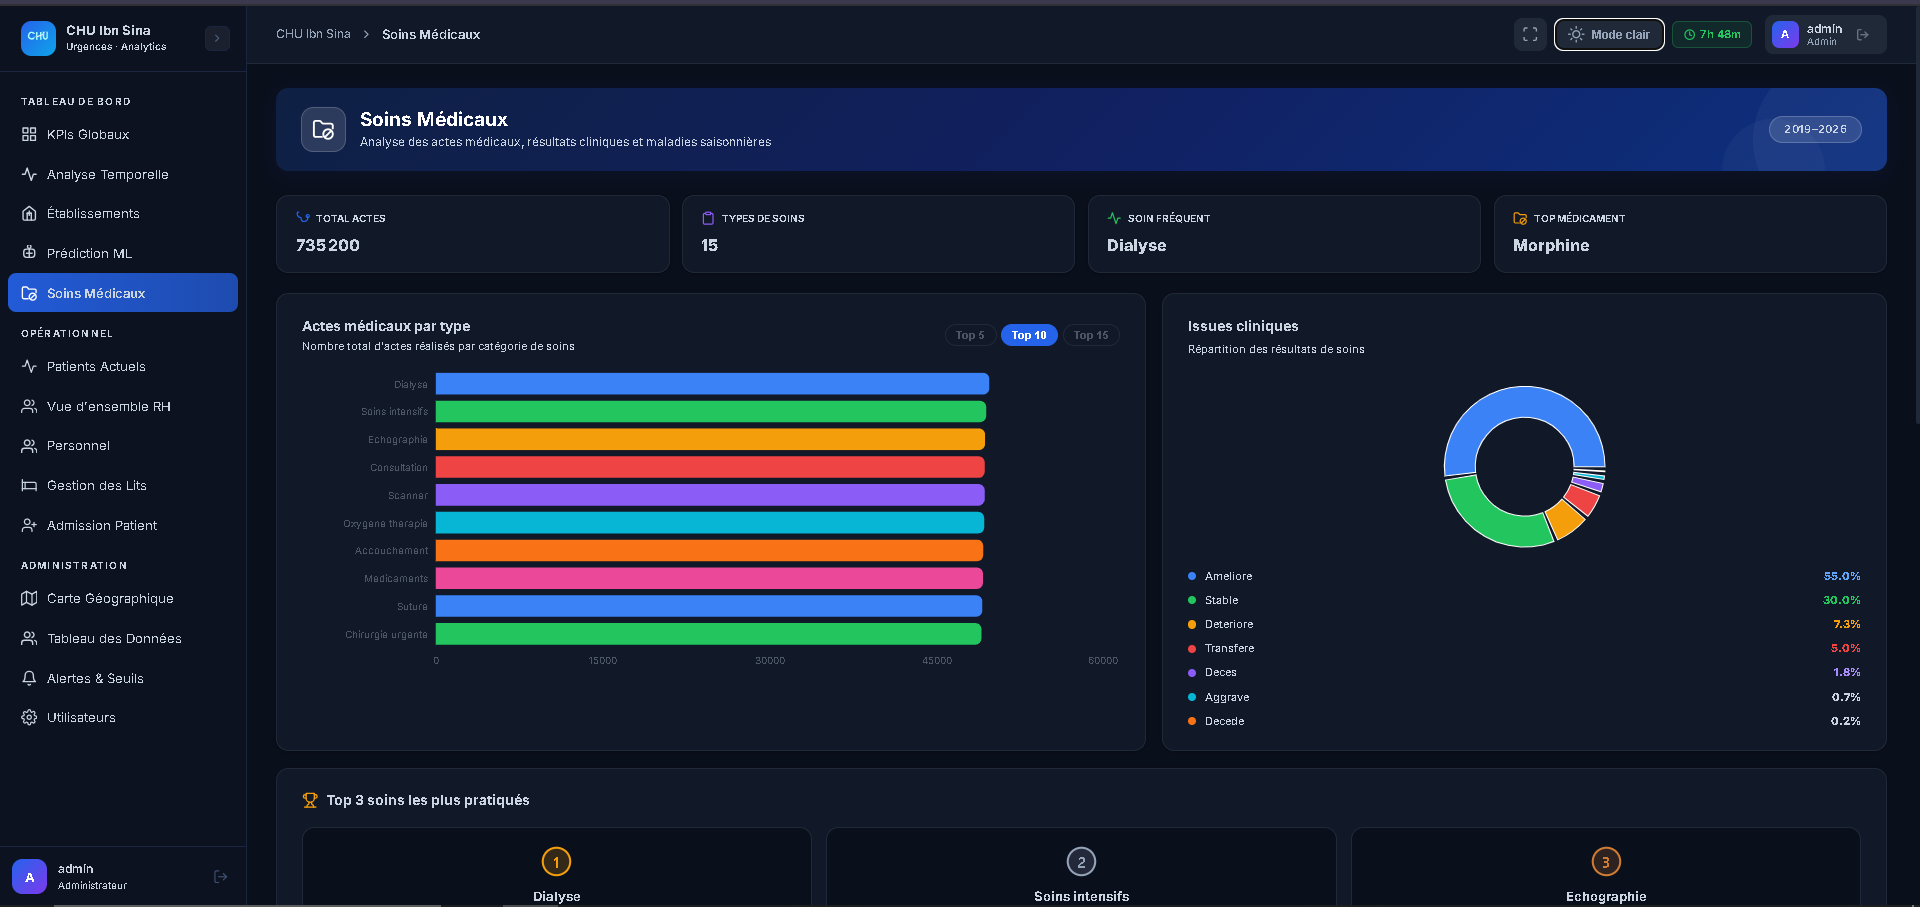
\includegraphics[width=\textwidth]{Soins medicaux.png}
			\caption{Soins Médicaux}
		\end{subfigure}
		\hfill
		\begin{subfigure}[b]{0.48\textwidth}
			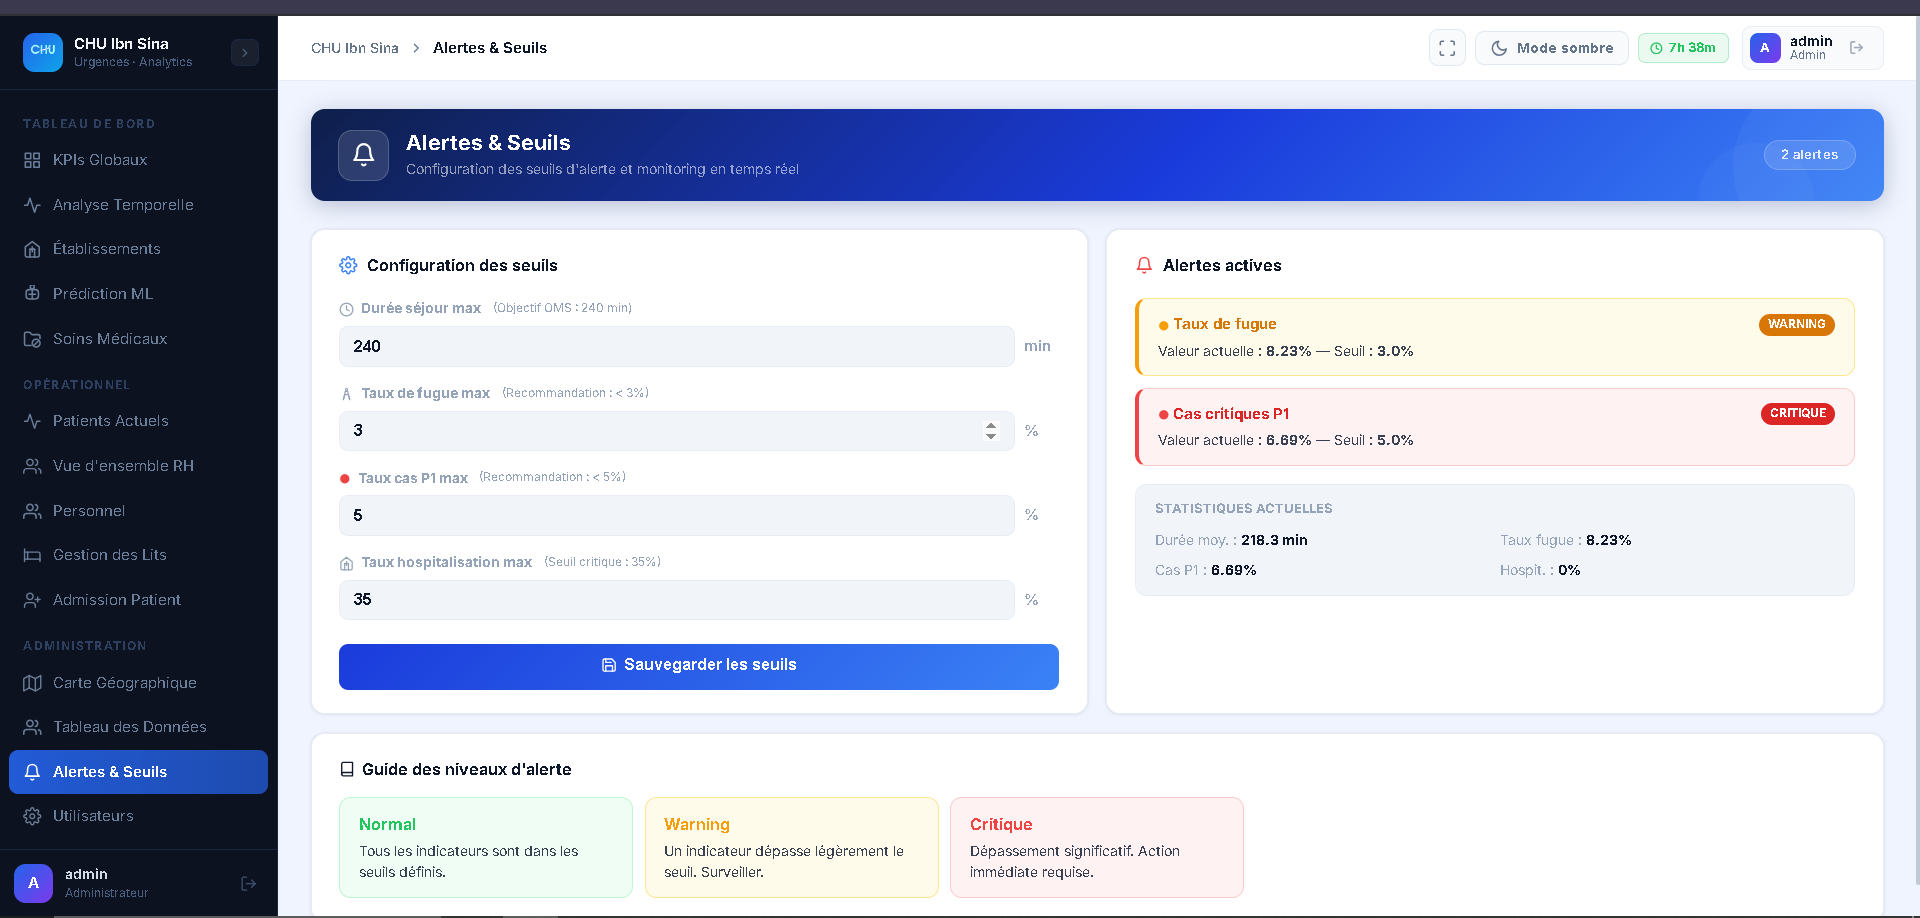
\includegraphics[width=\textwidth]{Alertes et Seuils.png}
			\caption{Alertes \& Seuils}
		\end{subfigure}
		
		\caption{Galerie des pages du tableau de bord CHU Ibn Sina}
	\end{figure}
	
	% ── Table des matières complète (chapitres + sections + sous-sections) ───────
	
	
	% ── Fin du document ──────────────────────────────────────────────────────────
\end{document}
